%!TEX root = mainfile.tex

\section{Introduction} % (fold)
\label{sec:introduction}
	Tomography is a technique for imaging objects and examining the internal structure of them in a non-invasive way. It is of enormous use in the medical industry where the ability to view the inside of a patient's body can be invaluable in the diagnostic process. Tomography stands out from other methods of viewing the internal structures of objects since it is able to view a slice through the object without the addition of the material around it in other slices, i.e.\ the rest of the object does not obscure the slice being viewed.

    Tomography can be applied to many different imaging techniques, x-ray, MRI and ultrasound, and has been applied to many areas of scientific study and research including medicine, chemistry, astronomy and geology.

    Tomographic reconstruction involves the creation of an image of an object taken through a particular slice by recombining the data collected from a set of line integrals across that object in the plane of interest. In other words, it is the conversion of a 3D averaged, or integrated, view of an object into a 2D slice of the object at a particular location, so that the details of the interior can be examined.

    The word tomography comes from the Greek \textit{tomos} meaning section and \textit{graphein} meaning to write, so tomography is simply writing `parts' of an object, in this case an image of a single plane through that object, in a useful form.
% section introduction (end)

\section{Tomographic Reconstruction} % (fold)
\label{sec:tomographic_reconstruction}
    In order to examine this method of image construction, we shall use a series of images which form \textit{sagittal} slices of a human head. This means that each of the 129 images in the collection are a slice from side to side at a slightly different position. Together, they form a 3 dimensional image of the head, with all of the interior detail maintained. A few of these images are shown in figure~\ref{fig:example_sagittal}
    \begin{figure}[ht]
        \centering
        \begin{minipage}[c]{0.19\linewidth}
            \centering
            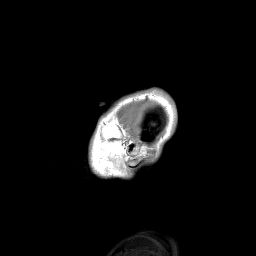
\includegraphics[width=\textwidth]{Files/report_images/sagittal_example1.jpg}
        \end{minipage}
        \begin{minipage}[c]{0.19\linewidth}
            \centering
            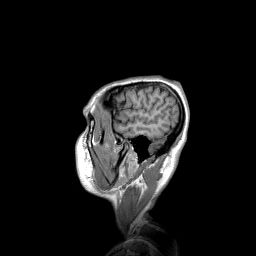
\includegraphics[width=\textwidth]{Files/report_images/sagittal_example2.jpg}
        \end{minipage}
        \begin{minipage}[c]{0.19\linewidth}
            \centering
            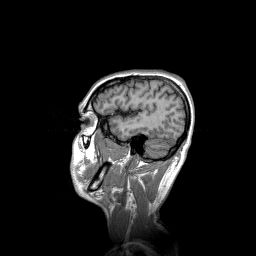
\includegraphics[width=\textwidth]{Files/report_images/sagittal_example3.jpg}
        \end{minipage}
        \begin{minipage}[c]{0.19\linewidth}
            \centering
            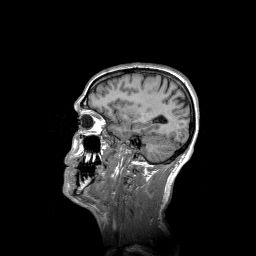
\includegraphics[width=\textwidth]{Files/report_images/sagittal_example4.jpg}
        \end{minipage}
        \begin{minipage}[c]{0.19\linewidth}
            \centering
            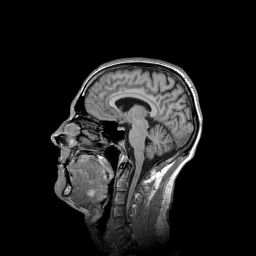
\includegraphics[width=\textwidth]{Files/report_images/sagittal_example5.jpg}
        \end{minipage}
        \caption{Example slices from the original sagittal 3D image that will be used to examine the tomographic reconstruction method. Out of the 129 images that make up the full image, these are, from left to right, image 20, 31. 38, 48 and 64 respectively.\label{fig:example_sagittal}}
    \end{figure}

    In order to demonstrate the tomographic reconstruction method as used in medical applications, an effective CT scan can be taken of this 3D image by converting it to axial slices. These are slices taken laterally through the object from top to bottom. Again, a selection of this new 3D image is shown in figure~\ref{fig:example_axial}.
    \begin{figure}[ht]
        \centering
        \begin{minipage}[c]{0.3\linewidth}
            \centering
            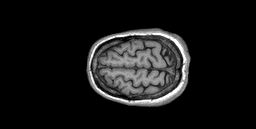
\includegraphics[width=\textwidth]{Files/report_images/axial_example1.jpg}
        \end{minipage}
        \begin{minipage}[c]{0.3\linewidth}
            \centering
            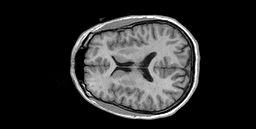
\includegraphics[width=\textwidth]{Files/report_images/axial_example2.jpg}
        \end{minipage}
        \begin{minipage}[c]{0.3\linewidth}
            \centering
            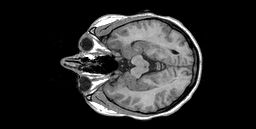
\includegraphics[width=\textwidth]{Files/report_images/axial_example3.jpg}
        \end{minipage}

        \begin{minipage}[c]{0.3\linewidth}
            \centering
            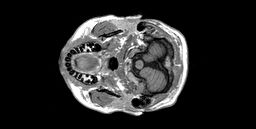
\includegraphics[width=\textwidth]{Files/report_images/axial_example4.jpg}
        \end{minipage}
        \begin{minipage}[c]{0.3\linewidth}
            \centering
            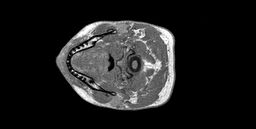
\includegraphics[width=\textwidth]{Files/report_images/axial_example5.jpg}
        \end{minipage}
        \begin{minipage}[c]{0.3\linewidth}
            \centering
            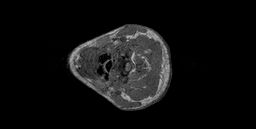
\includegraphics[width=\textwidth]{Files/report_images/axial_example6.jpg}
        \end{minipage}
        \caption{Example slices from the original sagittal 3D image that will be used to examine the tomographic reconstruction method. Out of the 129 images that make up the full image, these are, from top left to bottom right, image 78, 106, 126, 162 and 182 respectively.\label{fig:example_axial}}
    \end{figure}

    In order to show the effectiveness of the different techniques used in tomographic reconstruction, we shall refer back to a single of these slices, which will be the one that shall be reconstructed. This reference image will be image NUM out of the 256 stack above, and is shown in figure~\ref{fig:reference_slice}.
    \begin{figure}[ht]
        \centering
        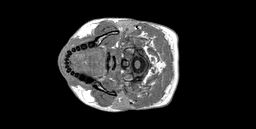
\includegraphics[width=0.4\textwidth]{Files/report_images/reference_slice.jpg}
        \caption{Reference slice that shall be used to compare later.\label{fig:reference_slice}}
    \end{figure}

    \subsection{Tomographic Scanner} % (fold)
    \label{sub:tomographic_scanner}
        When used in medical imaging applications, the data that is collected by a tomographic scanner would be represented by the image in figure~\ref{fig:3d_scan_example}.
        \begin{figure}[ht]
            \centering
                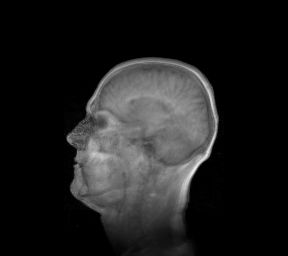
\includegraphics[width=0.4\textwidth]{Files/report_images/3D_scan_example.jpg}
            \caption{An image of the 3 dimensional representation of an object that would be measured by a tomographic scanner. This is just one view of the $360^{\circ}$ image that is generated.\label{fig:3d_scan_example}}
        \end{figure}

        The full image consists of a number of views of the object, each showing what it looks like from a different angle, averaged or integrated over its depth. Tomographic reconstruction involves calculating the reference image above, starting from this 3D representation
    % subsection tomographic_scanner (end)
% section tomographic_reconstruction (end)

\section{Back Projection} % (fold)
\label{sec:back_projection}
    The general method for tomographic reconstruction is called back projection. There are number of variations on this method that provide varying quality of results. We shall first examine the basic method of back projection and then see how it can be improved to increase the accuracy of the images calculated with it.

    \subsection{Sinogram} % (fold)
    \label{sub:sinogram}
        Since we now have a 3D image, such as would be collected when imaging an object from a large number of different angles around it, we can no longer determine what the interior contains. The first step to finding this is the plot a sinogram. Each slide of the 3D image is a view of the object from a particular angle. Since we require to see the interior of the object only through a particular single slice, most of the 3D image is not needed. Thus the useful information is a series of single pixel tall images of a single slice of the object taken at slightly different angle around it.

        A sinogram is a combined image of all of these views plotted as the value of the line integral with $x'$ against the angle $theta$, as per the diagram in figure~\ref{fig:sinogram_diag}. Since the different views are all taken about a single static point, polar co-ordinates are used, such that
        \begin{align}
            x\cos(\theta) + y\sin(\theta) = x'
        \end{align}
        Thus, the set of measurements that are collected for a given angle, $\theta$, make up a single layer of figure~\ref{fig:example_sinogram} and are called the parallel projection of the object at the angle $\theta$, denoted as $P_{\theta}(x')$.
        \begin{figure}[ht]
            \begin{center}
                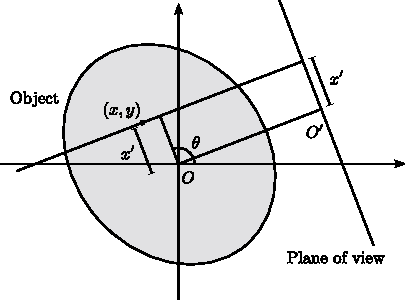
\includegraphics[width=0.5\textwidth]{Files/report_images/sinogram_diag.pdf}
            \end{center}
            \caption{A sinogram is an image of the value of the line integral plotted against angle for all the views around a measured object. Each point from the object traces a sinusoidal line as the angle is increased, or as the object is rotated in front of the measuring device. Angle is represented on the vertical axis and the position $x'$ on the horizontal.\label{fig:sinogram_diag}}
        \end{figure}

        An example of a sinogram, showing the plot for the data concerning the slice that holds the information for the reference image above, is shown in figure~\ref{fig:example_sinogram}.
        \begin{figure}[ht]
            \begin{center}
                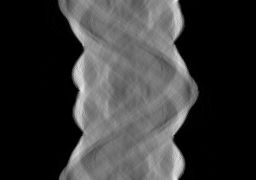
\includegraphics[width=0.4\textwidth]{Files/report_images/example_sinograph.jpg}
            \end{center}
            \caption{A sinogram is an image of the value of the line integral plotted against angle for all the views around a measured object. Each point from the object traces a sinusoidal line as the angle is increased, or as the object is rotated in front of the measuring device.\label{fig:example_sinogram}}
        \end{figure}

        \subsubsection{Radon Transform} % (fold)
        \label{ssub:radon_transform}
            The mathematical operation that gives the sinogram of an imaged slice is called the Radon Transform, ``it is the integral transform consisting of the integral of a function over straight lines''. In other words, the Radon Transform is the line integral along each of the possible straight lines defined over the area of the space represented by the original function. The transform is defined over the line space, $L$, as
            \begin{align}
                R_f(L) &= \int_L f(\boldsymbol{r})|\d{\boldsymbol{r}}|
            \end{align}
            Any stright line through the original function space can be defined in polar co-ordinates given a point through which the line passes and an angle $\theta$, that the line subtends. If the line passes through the point $(x,y)$, then any line can be defined as
            \begin{align}
                (x,y) &= \Big(\big[x'\cos(\theta)+y'\sin(\theta)\big], \big[-y'\cos(\theta)+x'\sin(\theta)\big]\Big)
            \end{align}
            where $x'$ is the distance of the line from the origin, as shown in figure~\ref{fig:sinogram_diag}. This means, then, that the Radon transform can be rewritted in terms of this general line form,
            \begin{align}
                R_f(\theta,x') &= \int_{-\infty}^{\infty} f(x,y)\d{t} \\
                &= \int_{-\infty}^{\infty} f\Big(\big[x'\cos(\theta)+y'\sin(\theta)\big], \big[-y'\cos(\theta)+x'\sin(\theta)\big]\Big)\d{t}
            \end{align}
            This means that every point in the original function is mapped to a location described by a combination of sine and cosine functions. This is clearly seen when considering the Radon Transform of several a Dirac Delta functions $\delta(x,y)$, which are described by the same number of sine waves with different phases, depending on their original position, as shown in figure~\ref{fig:delta_radon_transform}.
            \begin{figure}[ht]
                \centering
                \begin{minipage}[c]{0.2\linewidth}
                    \centering
                    
\includegraphics[width=\textwidth]{Files/report_images/radon_transform_deltas_original.png}
                \end{minipage}
                ~
                \begin{minipage}[c]{0.5\linewidth}
                    \centering
                    
\includegraphics[width=\textwidth]{Files/report_images/radon_transform_deltas.png}
                \end{minipage}
                \caption{The Radon Transform (left) of a series of finite delta functions (right). The Radon Transform can be thought of as the project of the original image as viewed from in the plane of the image, as the field of view is rotated around the image. The horizontal axis is now representing angle and vertical position.\label{fig:delta_radon_transform}}
            \end{figure}

            When this transform is applied to more complex images, the result is a very large number of blurred sine waves with different phases and also different amplitudes that, together, represent the whole image.
        % subsubsection radon_transform (end)
        \subsection{Back Projection Algorithm} % (fold)
        \label{sub:back_projection_algorithm}
            The basic steps when reconstructing the axial slice from the sinogram using back projection are as follows
            \begin{enumerate}
                \item Take the measured line integral at each offset along the projection
                \item Spread this value back uniformly along the line of measurement
                \item Repeat for every projection taken at all angles around the object
                \item Sum the contributions from all of the projections to give a back-projected reconstruction of the axial slice.
            \end{enumerate}

            This process is simple and computationally simple. However, this method produces serious artefacts making the image only just recognisable as the desired reconstruction, when compared to the reference image above, as shown in figure~\ref{fig:simple_backprojection}.
            \begin{figure}[ht]
                \begin{center}
                    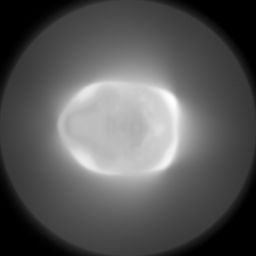
\includegraphics[width=0.4\textwidth]{Files/report_images/simple_backprojection.jpg}
                \end{center}
                \caption{The reconstructed axial slice using only basic back projection. The image is just recognisable as being related to the reference image, but there are severe artefacts and tails making any application of this image almost useless.\label{fig:simple_backprojection}}
            \end{figure}

            The reason the image looks so blurred, with so much extra information, is that the back-projections of each individual linear projection are summed over the full width and heigh of the image. This means that, although most, if not all, of the original information is concentrated in the centre of the image, this is spread out to include the edges, simply because there is nothing to tell the algorithm not to, and so the tails are spread back to the extremities of the image.

            We shall consider some methods for improving this image.
        % subsection back_projection_algorithm (end)
    % subsection sinogram (end)
% section back_projection (end)

\section{Central Slice Theorem} % (fold)
\label{sec:central_slice_theorem}
    The back projection method works, insofar as we now have an image, reconstructed from the 3D scan that is recognisable as the reference image in figure~\ref{fig:reference_slice}. However we want to improve the algorithm, so that it does not trace the projections back uniformly which leads to the long tails shown above. One method of doing this involves the central slice theorem.

    The Central Slice Theorem states that the results of the following two calculations are equal:
    \begin{itemize}
        \item Take a two-dimensional function $f(\boldsymbol{r})$, project it onto a one-dimensional line, and do a Fourier transform of that projection.
        \item Take that same function, but do a two-dimensional Fourier transform first, and then take a single slice through the origin, which is parallel to the projection line.
    \end{itemize}

    This theorem means that we can use each row of the sinogram to build the 2D Fourier Transform of the axial slice since the 1D Fourier Transform of each row forms a radial (central) slice of the 2D transform.
    \begin{figure}[ht]
        \begin{center}
            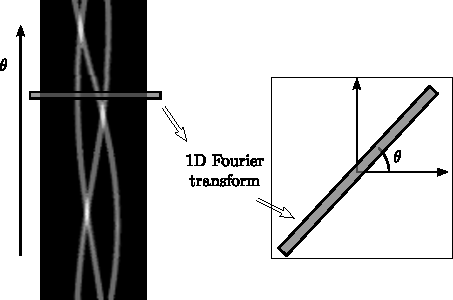
\includegraphics[width=0.6\textwidth]{Files/report_images/central_slice_theorem.pdf}
        \end{center}
        \caption{The central slice theorem means that the 2D Fourier Transform of the final image can be constructed from the 1D transforms of each slice of the sinogram.\label{fig:central_slice_theorem}}
    \end{figure}

    However, if this method is used to compute the axial slice, the same image as previously is found, with the tails and severe artefacts. This is because taking the Fourier Transform is a linear operation. This means that the steps taken here, taking the Fourier Transform (FT), adding the images and then taking the inverse FT is identical as adding the images and then taking the FT then the inverse FT. Since taking the FT and then inverse FT will clearly give the same original image, this is the same as before when just adding the back projections.

    The reason that there was no improvement in  final image quality is due to the distribution of samples of the Fourier Transform. Moving radially outward from the centre of the image, the sample density decreases as $\frac{1}{|r|}$, where $r$ is the radius. To correct for this, a weighting factor must be used to make the FT uniform in sample density. This is performed either in frequency space once the FT has been taken, before the inverse, or in real space.

    The weighting factor is usually applied in real space as this proves to be less computationally intensive. This is possible because multiplying each central slice by the weighting factor is the same as convolving the inverse FT of each slice with the inverse FT of the weighting factor.

    We can demonstrate this by considering the Fourier Transform for both cases. The general function, $f(x,y)$ can be obtained from its Fourier Transform $F(k_x,k_y)$ by the inverse transform,
    \begin{align}
        f(x,y) &= \int_{-\infty}^{\infty}\int_{-\infty}^{\infty} F(k_x,k_y)\e{ik_x x+ik_y y} \d{k_x}\d{k_y}
    \end{align}
    Since the central slice theorem is defined through the centre of the transform, it is convenient to use polar coordinates, though with ranges $-\infty < k < \infty$ and $0 < \theta < \pi$,
    \begin{align}
        f(x,y) &= \int_{0}^{\pi}\int_{-\infty}^{\infty}F(k,\theta)|k|\e{ik(x\cos\theta + y\sin\theta)} \d{k}\d{\theta}
    \end{align}
    If we define $F(k,\theta) = Q_{\theta}(k)$, where $Q_{\theta}$ is the Fourier Transform of the projection $P_{\theta}$, then we have,
    \begin{align}
        f(x,y) &= \int_{0}^{\pi}\left\{\int_{-\infty}^{\infty}Q_{\theta}(k)|k|\e{ik(x\cos\theta + y\sin\theta)} \d{k}\right\}\d{\theta} \\
        &= \int_{0}^{\pi}\underbrace{\int_{-\infty}^{\infty}Q_{\theta}(k)|k|\e{ikx'} \d{k}}_\text{A}\d{\theta} \label{eq:filtered_backprojection}
    \end{align}
    This means that the image $f(x,y)$ can be found by back projecting part A of equation~\ref{eq:filtered_backprojection}. Part A is the inverse Fourier Transform of the two functions $Q_{\theta}$ and $|k|$, and so, since $Q_{\theta}$ is the the FT of $P_{\theta}$, A can be expressed as the convolution of $P_{\theta}$ with a filter given by the inverse FT of the weighting function. All that remains, then, in order to perform the reconstruction is to find the filter, given by the inverse FT of the weighting function. The 2D Fourier Transform of $\frac{1}{r}$ is $\frac{1}{|k|}$, and so the weighting function that is used as the filter is the inverse FT of $|k|$.

    \subsection{Filter} % (fold)
    \label{sub:filter}
        The function that we need to use as the filter, in order to correct for the changes in density of the FT sampling, is the inverse FT of the function $|k|$. When considering the whole plane, from $-\infty < k < \infty$, this solution does not exist as the series diverges. But there is a maximum frequency, $k_\max$, that is of interest, the Nyquist Frequency, outside of which the information can be discarded, and so the function can be redefined as
        \begin{align}
            f(k) =
                \begin{cases}
                    |k| & |k| < k{_\max} \\
                    0   & |k| > {_\max}
                \end{cases}
        \end{align}
        The inverse FT for this function is defined as
        \begin{align}
            f(x) &= k^2_{\max} \left[ \frac{2\sin(2\pi xk_{\max})}{2\pi xk_{\max}} - \left( \frac{\sin(\pi xk_{\max})}{\pi xk_{\max}} \right)^2 \right]
        \end{align}
        This can be adapted for use when the function is discretised. So for $k_\max =\frac{1}{2D}$, where $D$ is the sampling interval, and $n=\frac{x}{D}$, the filter becomes
        \begin{align}
            f(n) &\propto \left[ \frac{2\sin(\pi n)}{\pi n} - \left( \frac{\sin(\frac{\pi n}{2})}{\frac{\pi n}{2}} \right)^2 \right]
        \end{align}
        and is shown plotted in figure~\ref{fig:filter_graph}.
        \begin{figure}[ht]
            \centering
                \begingroup\endlinechar=-1
                \resizebox{0.7\textwidth}{!}{%
                    % GNUPLOT: LaTeX picture
\setlength{\unitlength}{0.240900pt}
\ifx\plotpoint\undefined\newsavebox{\plotpoint}\fi
\sbox{\plotpoint}{\rule[-0.200pt]{0.400pt}{0.400pt}}%
\begin{picture}(1500,900)(0,0)
\sbox{\plotpoint}{\rule[-0.200pt]{0.400pt}{0.400pt}}%
\put(130.0,82.0){\rule[-0.200pt]{4.818pt}{0.400pt}}
\put(110,82){\makebox(0,0)[r]{-0.6}}
\put(1419.0,82.0){\rule[-0.200pt]{4.818pt}{0.400pt}}
\put(130.0,179.0){\rule[-0.200pt]{4.818pt}{0.400pt}}
\put(110,179){\makebox(0,0)[r]{-0.4}}
\put(1419.0,179.0){\rule[-0.200pt]{4.818pt}{0.400pt}}
\put(130.0,276.0){\rule[-0.200pt]{4.818pt}{0.400pt}}
\put(110,276){\makebox(0,0)[r]{-0.2}}
\put(1419.0,276.0){\rule[-0.200pt]{4.818pt}{0.400pt}}
\put(130.0,373.0){\rule[-0.200pt]{4.818pt}{0.400pt}}
\put(110,373){\makebox(0,0)[r]{ 0}}
\put(1419.0,373.0){\rule[-0.200pt]{4.818pt}{0.400pt}}
\put(130.0,471.0){\rule[-0.200pt]{4.818pt}{0.400pt}}
\put(110,471){\makebox(0,0)[r]{ 0.2}}
\put(1419.0,471.0){\rule[-0.200pt]{4.818pt}{0.400pt}}
\put(130.0,568.0){\rule[-0.200pt]{4.818pt}{0.400pt}}
\put(110,568){\makebox(0,0)[r]{ 0.4}}
\put(1419.0,568.0){\rule[-0.200pt]{4.818pt}{0.400pt}}
\put(130.0,665.0){\rule[-0.200pt]{4.818pt}{0.400pt}}
\put(110,665){\makebox(0,0)[r]{ 0.6}}
\put(1419.0,665.0){\rule[-0.200pt]{4.818pt}{0.400pt}}
\put(130.0,762.0){\rule[-0.200pt]{4.818pt}{0.400pt}}
\put(110,762){\makebox(0,0)[r]{ 0.8}}
\put(1419.0,762.0){\rule[-0.200pt]{4.818pt}{0.400pt}}
\put(130.0,859.0){\rule[-0.200pt]{4.818pt}{0.400pt}}
\put(110,859){\makebox(0,0)[r]{ 1}}
\put(1419.0,859.0){\rule[-0.200pt]{4.818pt}{0.400pt}}
\put(130.0,82.0){\rule[-0.200pt]{0.400pt}{4.818pt}}
\put(130,41){\makebox(0,0){-10}}
\put(130.0,839.0){\rule[-0.200pt]{0.400pt}{4.818pt}}
\put(457.0,82.0){\rule[-0.200pt]{0.400pt}{4.818pt}}
\put(457,41){\makebox(0,0){-5}}
\put(457.0,839.0){\rule[-0.200pt]{0.400pt}{4.818pt}}
\put(785.0,82.0){\rule[-0.200pt]{0.400pt}{4.818pt}}
\put(785,41){\makebox(0,0){ 0}}
\put(785.0,839.0){\rule[-0.200pt]{0.400pt}{4.818pt}}
\put(1112.0,82.0){\rule[-0.200pt]{0.400pt}{4.818pt}}
\put(1112,41){\makebox(0,0){ 5}}
\put(1112.0,839.0){\rule[-0.200pt]{0.400pt}{4.818pt}}
\put(1439.0,82.0){\rule[-0.200pt]{0.400pt}{4.818pt}}
\put(1439,41){\makebox(0,0){ 10}}
\put(1439.0,839.0){\rule[-0.200pt]{0.400pt}{4.818pt}}
\put(130.0,82.0){\rule[-0.200pt]{0.400pt}{187.179pt}}
\put(130.0,82.0){\rule[-0.200pt]{315.338pt}{0.400pt}}
\put(1439.0,82.0){\rule[-0.200pt]{0.400pt}{187.179pt}}
\put(130.0,859.0){\rule[-0.200pt]{315.338pt}{0.400pt}}
\put(130,373){\usebox{\plotpoint}}
\put(130,373){\usebox{\plotpoint}}
\put(130,373){\usebox{\plotpoint}}
\put(130,373){\usebox{\plotpoint}}
\put(130,373){\usebox{\plotpoint}}
\put(130,373){\usebox{\plotpoint}}
\put(130,373){\usebox{\plotpoint}}
\put(130,373){\usebox{\plotpoint}}
\put(130,373){\usebox{\plotpoint}}
\put(130,373){\usebox{\plotpoint}}
\put(130,373){\usebox{\plotpoint}}
\put(130,373){\usebox{\plotpoint}}
\put(130,373){\usebox{\plotpoint}}
\put(130,373){\usebox{\plotpoint}}
\put(130,373){\usebox{\plotpoint}}
\put(130,373){\usebox{\plotpoint}}
\put(130,373){\usebox{\plotpoint}}
\put(130,373){\usebox{\plotpoint}}
\put(130,373){\usebox{\plotpoint}}
\put(130,373){\usebox{\plotpoint}}
\put(130,373){\usebox{\plotpoint}}
\put(130,373){\usebox{\plotpoint}}
\put(130,373){\usebox{\plotpoint}}
\put(130,373){\usebox{\plotpoint}}
\put(130,373){\usebox{\plotpoint}}
\put(130,373){\usebox{\plotpoint}}
\put(130,373){\usebox{\plotpoint}}
\put(130,373){\usebox{\plotpoint}}
\put(130,373){\usebox{\plotpoint}}
\put(130,373){\usebox{\plotpoint}}
\put(130,373){\usebox{\plotpoint}}
\put(130,373){\usebox{\plotpoint}}
\put(130,373){\usebox{\plotpoint}}
\put(130,373){\usebox{\plotpoint}}
\put(130,373){\usebox{\plotpoint}}
\put(130,373){\usebox{\plotpoint}}
\put(130,373){\usebox{\plotpoint}}
\put(130,373){\usebox{\plotpoint}}
\put(130,373){\usebox{\plotpoint}}
\put(130.0,373.0){\usebox{\plotpoint}}
\put(131.0,371.0){\rule[-0.200pt]{0.400pt}{0.482pt}}
\put(131.0,371.0){\usebox{\plotpoint}}
\put(132.0,370.0){\usebox{\plotpoint}}
\put(132.0,370.0){\usebox{\plotpoint}}
\put(133.0,368.0){\rule[-0.200pt]{0.400pt}{0.482pt}}
\put(133.0,368.0){\usebox{\plotpoint}}
\put(134.0,367.0){\usebox{\plotpoint}}
\put(134.0,367.0){\usebox{\plotpoint}}
\put(135.0,365.0){\rule[-0.200pt]{0.400pt}{0.482pt}}
\put(135.0,365.0){\usebox{\plotpoint}}
\put(136.0,364.0){\usebox{\plotpoint}}
\put(136.0,364.0){\usebox{\plotpoint}}
\put(137.0,362.0){\rule[-0.200pt]{0.400pt}{0.482pt}}
\put(137.0,362.0){\usebox{\plotpoint}}
\put(138.0,361.0){\usebox{\plotpoint}}
\put(138.0,361.0){\usebox{\plotpoint}}
\put(139.0,359.0){\rule[-0.200pt]{0.400pt}{0.482pt}}
\put(139.0,359.0){\usebox{\plotpoint}}
\put(140.0,358.0){\usebox{\plotpoint}}
\put(140.0,358.0){\usebox{\plotpoint}}
\put(141.0,357.0){\usebox{\plotpoint}}
\put(141.0,357.0){\usebox{\plotpoint}}
\put(142.0,355.0){\rule[-0.200pt]{0.400pt}{0.482pt}}
\put(142.0,355.0){\usebox{\plotpoint}}
\put(143.0,354.0){\usebox{\plotpoint}}
\put(143.0,354.0){\usebox{\plotpoint}}
\put(144.0,353.0){\usebox{\plotpoint}}
\put(144.0,353.0){\usebox{\plotpoint}}
\put(145.0,352.0){\usebox{\plotpoint}}
\put(145.0,352.0){\usebox{\plotpoint}}
\put(146,349.67){\rule{0.241pt}{0.400pt}}
\multiput(146.00,350.17)(0.500,-1.000){2}{\rule{0.120pt}{0.400pt}}
\put(146.0,351.0){\usebox{\plotpoint}}
\put(147,350){\usebox{\plotpoint}}
\put(147,350){\usebox{\plotpoint}}
\put(147,350){\usebox{\plotpoint}}
\put(147,350){\usebox{\plotpoint}}
\put(147,350){\usebox{\plotpoint}}
\put(147,350){\usebox{\plotpoint}}
\put(147,350){\usebox{\plotpoint}}
\put(147,350){\usebox{\plotpoint}}
\put(147,350){\usebox{\plotpoint}}
\put(147,350){\usebox{\plotpoint}}
\put(147,350){\usebox{\plotpoint}}
\put(147,350){\usebox{\plotpoint}}
\put(147,350){\usebox{\plotpoint}}
\put(147,350){\usebox{\plotpoint}}
\put(147,350){\usebox{\plotpoint}}
\put(147,350){\usebox{\plotpoint}}
\put(147,350){\usebox{\plotpoint}}
\put(147,350){\usebox{\plotpoint}}
\put(147,350){\usebox{\plotpoint}}
\put(147,350){\usebox{\plotpoint}}
\put(147,350){\usebox{\plotpoint}}
\put(147,350){\usebox{\plotpoint}}
\put(147,350){\usebox{\plotpoint}}
\put(147,350){\usebox{\plotpoint}}
\put(147,350){\usebox{\plotpoint}}
\put(147,350){\usebox{\plotpoint}}
\put(147,350){\usebox{\plotpoint}}
\put(147,350){\usebox{\plotpoint}}
\put(147,350){\usebox{\plotpoint}}
\put(147,350){\usebox{\plotpoint}}
\put(147,350){\usebox{\plotpoint}}
\put(147,350){\usebox{\plotpoint}}
\put(147,350){\usebox{\plotpoint}}
\put(147,350){\usebox{\plotpoint}}
\put(147,350){\usebox{\plotpoint}}
\put(147,350){\usebox{\plotpoint}}
\put(147,350){\usebox{\plotpoint}}
\put(147,350){\usebox{\plotpoint}}
\put(147,350){\usebox{\plotpoint}}
\put(147,350){\usebox{\plotpoint}}
\put(147,350){\usebox{\plotpoint}}
\put(147,350){\usebox{\plotpoint}}
\put(147,350){\usebox{\plotpoint}}
\put(147,350){\usebox{\plotpoint}}
\put(147,350){\usebox{\plotpoint}}
\put(147,350){\usebox{\plotpoint}}
\put(147,350){\usebox{\plotpoint}}
\put(147,350){\usebox{\plotpoint}}
\put(147,350){\usebox{\plotpoint}}
\put(147,350){\usebox{\plotpoint}}
\put(147,350){\usebox{\plotpoint}}
\put(147,350){\usebox{\plotpoint}}
\put(147,350){\usebox{\plotpoint}}
\put(147,350){\usebox{\plotpoint}}
\put(147,350){\usebox{\plotpoint}}
\put(147,350){\usebox{\plotpoint}}
\put(147,350){\usebox{\plotpoint}}
\put(147,350){\usebox{\plotpoint}}
\put(147,350){\usebox{\plotpoint}}
\put(147,350){\usebox{\plotpoint}}
\put(147,350){\usebox{\plotpoint}}
\put(147,350){\usebox{\plotpoint}}
\put(147,350){\usebox{\plotpoint}}
\put(147,350){\usebox{\plotpoint}}
\put(147,350){\usebox{\plotpoint}}
\put(147,350){\usebox{\plotpoint}}
\put(147,350){\usebox{\plotpoint}}
\put(147.0,349.0){\usebox{\plotpoint}}
\put(147.0,349.0){\usebox{\plotpoint}}
\put(148.0,348.0){\usebox{\plotpoint}}
\put(148.0,348.0){\usebox{\plotpoint}}
\put(149.0,347.0){\usebox{\plotpoint}}
\put(149.0,347.0){\usebox{\plotpoint}}
\put(150.0,346.0){\usebox{\plotpoint}}
\put(150.0,346.0){\usebox{\plotpoint}}
\put(151.0,345.0){\usebox{\plotpoint}}
\put(151.0,345.0){\rule[-0.200pt]{0.482pt}{0.400pt}}
\put(153.0,344.0){\usebox{\plotpoint}}
\put(153.0,344.0){\usebox{\plotpoint}}
\put(154.0,343.0){\usebox{\plotpoint}}
\put(154.0,343.0){\usebox{\plotpoint}}
\put(155.0,342.0){\usebox{\plotpoint}}
\put(155.0,342.0){\rule[-0.200pt]{0.482pt}{0.400pt}}
\put(157.0,341.0){\usebox{\plotpoint}}
\put(157.0,341.0){\rule[-0.200pt]{0.482pt}{0.400pt}}
\put(159.0,340.0){\usebox{\plotpoint}}
\put(159.0,340.0){\rule[-0.200pt]{2.409pt}{0.400pt}}
\put(169.0,340.0){\usebox{\plotpoint}}
\put(169.0,341.0){\rule[-0.200pt]{0.482pt}{0.400pt}}
\put(171.0,341.0){\usebox{\plotpoint}}
\put(171.0,342.0){\rule[-0.200pt]{0.482pt}{0.400pt}}
\put(173.0,342.0){\usebox{\plotpoint}}
\put(173.0,343.0){\usebox{\plotpoint}}
\put(174.0,343.0){\usebox{\plotpoint}}
\put(174.0,344.0){\rule[-0.200pt]{0.482pt}{0.400pt}}
\put(176.0,344.0){\usebox{\plotpoint}}
\put(176.0,345.0){\usebox{\plotpoint}}
\put(177.0,345.0){\usebox{\plotpoint}}
\put(177.0,346.0){\usebox{\plotpoint}}
\put(178.0,346.0){\usebox{\plotpoint}}
\put(178.0,347.0){\usebox{\plotpoint}}
\put(179.0,347.0){\usebox{\plotpoint}}
\put(179.0,348.0){\usebox{\plotpoint}}
\put(180.0,348.0){\usebox{\plotpoint}}
\put(180.0,349.0){\usebox{\plotpoint}}
\put(181.0,349.0){\usebox{\plotpoint}}
\put(181.0,350.0){\usebox{\plotpoint}}
\put(182.0,350.0){\rule[-0.200pt]{0.400pt}{0.482pt}}
\put(182.0,352.0){\usebox{\plotpoint}}
\put(183.0,352.0){\usebox{\plotpoint}}
\put(183.0,353.0){\usebox{\plotpoint}}
\put(184.0,353.0){\usebox{\plotpoint}}
\put(184.0,354.0){\usebox{\plotpoint}}
\put(185.0,354.0){\rule[-0.200pt]{0.400pt}{0.482pt}}
\put(185.0,356.0){\usebox{\plotpoint}}
\put(186.0,356.0){\usebox{\plotpoint}}
\put(186.0,357.0){\usebox{\plotpoint}}
\put(187.0,357.0){\usebox{\plotpoint}}
\put(187.0,358.0){\usebox{\plotpoint}}
\put(188.0,358.0){\rule[-0.200pt]{0.400pt}{0.482pt}}
\put(188.0,360.0){\usebox{\plotpoint}}
\put(189.0,360.0){\usebox{\plotpoint}}
\put(189.0,361.0){\usebox{\plotpoint}}
\put(190.0,361.0){\rule[-0.200pt]{0.400pt}{0.482pt}}
\put(190.0,363.0){\usebox{\plotpoint}}
\put(191.0,363.0){\rule[-0.200pt]{0.400pt}{0.482pt}}
\put(191.0,365.0){\usebox{\plotpoint}}
\put(192.0,365.0){\usebox{\plotpoint}}
\put(192.0,366.0){\usebox{\plotpoint}}
\put(193.0,366.0){\rule[-0.200pt]{0.400pt}{0.482pt}}
\put(193.0,368.0){\usebox{\plotpoint}}
\put(194.0,368.0){\usebox{\plotpoint}}
\put(194.0,369.0){\usebox{\plotpoint}}
\put(195.0,369.0){\rule[-0.200pt]{0.400pt}{0.482pt}}
\put(195.0,371.0){\usebox{\plotpoint}}
\put(196.0,371.0){\rule[-0.200pt]{0.400pt}{0.482pt}}
\put(196.0,373.0){\usebox{\plotpoint}}
\put(197.0,373.0){\usebox{\plotpoint}}
\put(197.0,374.0){\usebox{\plotpoint}}
\put(198.0,374.0){\rule[-0.200pt]{0.400pt}{0.482pt}}
\put(198.0,376.0){\usebox{\plotpoint}}
\put(199.0,376.0){\rule[-0.200pt]{0.400pt}{0.482pt}}
\put(199.0,378.0){\usebox{\plotpoint}}
\put(200.0,378.0){\usebox{\plotpoint}}
\put(200.0,379.0){\usebox{\plotpoint}}
\put(201.0,379.0){\rule[-0.200pt]{0.400pt}{0.482pt}}
\put(201.0,381.0){\usebox{\plotpoint}}
\put(202,381.67){\rule{0.241pt}{0.400pt}}
\multiput(202.00,381.17)(0.500,1.000){2}{\rule{0.120pt}{0.400pt}}
\put(202.0,381.0){\usebox{\plotpoint}}
\put(203,383){\usebox{\plotpoint}}
\put(203,383){\usebox{\plotpoint}}
\put(203,383){\usebox{\plotpoint}}
\put(203,383){\usebox{\plotpoint}}
\put(203,383){\usebox{\plotpoint}}
\put(203,383){\usebox{\plotpoint}}
\put(203,383){\usebox{\plotpoint}}
\put(203,383){\usebox{\plotpoint}}
\put(203,383){\usebox{\plotpoint}}
\put(203,383){\usebox{\plotpoint}}
\put(203,383){\usebox{\plotpoint}}
\put(203,383){\usebox{\plotpoint}}
\put(203,383){\usebox{\plotpoint}}
\put(203,383){\usebox{\plotpoint}}
\put(203,383){\usebox{\plotpoint}}
\put(203,383){\usebox{\plotpoint}}
\put(203,383){\usebox{\plotpoint}}
\put(203,383){\usebox{\plotpoint}}
\put(203,383){\usebox{\plotpoint}}
\put(203,383){\usebox{\plotpoint}}
\put(203,383){\usebox{\plotpoint}}
\put(203,383){\usebox{\plotpoint}}
\put(203,383){\usebox{\plotpoint}}
\put(203,383){\usebox{\plotpoint}}
\put(203,383){\usebox{\plotpoint}}
\put(203,383){\usebox{\plotpoint}}
\put(203,383){\usebox{\plotpoint}}
\put(203,383){\usebox{\plotpoint}}
\put(203,383){\usebox{\plotpoint}}
\put(203,383){\usebox{\plotpoint}}
\put(203,383){\usebox{\plotpoint}}
\put(203,383){\usebox{\plotpoint}}
\put(203,383){\usebox{\plotpoint}}
\put(203,383){\usebox{\plotpoint}}
\put(203,383){\usebox{\plotpoint}}
\put(203,383){\usebox{\plotpoint}}
\put(203,383){\usebox{\plotpoint}}
\put(203,383){\usebox{\plotpoint}}
\put(203,383){\usebox{\plotpoint}}
\put(203,383){\usebox{\plotpoint}}
\put(203,383){\usebox{\plotpoint}}
\put(203,383){\usebox{\plotpoint}}
\put(203,383){\usebox{\plotpoint}}
\put(203,383){\usebox{\plotpoint}}
\put(203,383){\usebox{\plotpoint}}
\put(203,383){\usebox{\plotpoint}}
\put(203,383){\usebox{\plotpoint}}
\put(203.0,383.0){\usebox{\plotpoint}}
\put(203.0,384.0){\usebox{\plotpoint}}
\put(204.0,384.0){\rule[-0.200pt]{0.400pt}{0.482pt}}
\put(204.0,386.0){\usebox{\plotpoint}}
\put(205.0,386.0){\usebox{\plotpoint}}
\put(205.0,387.0){\usebox{\plotpoint}}
\put(206.0,387.0){\rule[-0.200pt]{0.400pt}{0.482pt}}
\put(206.0,389.0){\usebox{\plotpoint}}
\put(207.0,389.0){\usebox{\plotpoint}}
\put(207.0,390.0){\usebox{\plotpoint}}
\put(208.0,390.0){\rule[-0.200pt]{0.400pt}{0.482pt}}
\put(208.0,392.0){\usebox{\plotpoint}}
\put(209.0,392.0){\usebox{\plotpoint}}
\put(209.0,393.0){\usebox{\plotpoint}}
\put(210.0,393.0){\usebox{\plotpoint}}
\put(210.0,394.0){\usebox{\plotpoint}}
\put(211.0,394.0){\rule[-0.200pt]{0.400pt}{0.482pt}}
\put(211.0,396.0){\usebox{\plotpoint}}
\put(212.0,396.0){\usebox{\plotpoint}}
\put(212.0,397.0){\usebox{\plotpoint}}
\put(213.0,397.0){\usebox{\plotpoint}}
\put(213.0,398.0){\usebox{\plotpoint}}
\put(214.0,398.0){\usebox{\plotpoint}}
\put(214.0,399.0){\usebox{\plotpoint}}
\put(215.0,399.0){\rule[-0.200pt]{0.400pt}{0.482pt}}
\put(215.0,401.0){\usebox{\plotpoint}}
\put(216.0,401.0){\usebox{\plotpoint}}
\put(216.0,402.0){\usebox{\plotpoint}}
\put(217.0,402.0){\usebox{\plotpoint}}
\put(217.0,403.0){\rule[-0.200pt]{0.482pt}{0.400pt}}
\put(219.0,403.0){\usebox{\plotpoint}}
\put(219.0,404.0){\usebox{\plotpoint}}
\put(220.0,404.0){\usebox{\plotpoint}}
\put(220.0,405.0){\usebox{\plotpoint}}
\put(221.0,405.0){\usebox{\plotpoint}}
\put(221.0,406.0){\rule[-0.200pt]{0.482pt}{0.400pt}}
\put(223.0,406.0){\usebox{\plotpoint}}
\put(223.0,407.0){\rule[-0.200pt]{0.482pt}{0.400pt}}
\put(225.0,407.0){\usebox{\plotpoint}}
\put(225.0,408.0){\rule[-0.200pt]{2.409pt}{0.400pt}}
\put(235.0,407.0){\usebox{\plotpoint}}
\put(235.0,407.0){\rule[-0.200pt]{0.482pt}{0.400pt}}
\put(237.0,406.0){\usebox{\plotpoint}}
\put(237.0,406.0){\usebox{\plotpoint}}
\put(238.0,405.0){\usebox{\plotpoint}}
\put(238.0,405.0){\usebox{\plotpoint}}
\put(239.0,404.0){\usebox{\plotpoint}}
\put(239.0,404.0){\rule[-0.200pt]{0.482pt}{0.400pt}}
\put(241.0,403.0){\usebox{\plotpoint}}
\put(241.0,403.0){\usebox{\plotpoint}}
\put(242.0,402.0){\usebox{\plotpoint}}
\put(242.0,402.0){\usebox{\plotpoint}}
\put(243.0,401.0){\usebox{\plotpoint}}
\put(243.0,401.0){\usebox{\plotpoint}}
\put(244.0,399.0){\rule[-0.200pt]{0.400pt}{0.482pt}}
\put(244.0,399.0){\usebox{\plotpoint}}
\put(245.0,398.0){\usebox{\plotpoint}}
\put(245.0,398.0){\usebox{\plotpoint}}
\put(246.0,397.0){\usebox{\plotpoint}}
\put(246.0,397.0){\usebox{\plotpoint}}
\put(247.0,396.0){\usebox{\plotpoint}}
\put(247.0,396.0){\usebox{\plotpoint}}
\put(248.0,394.0){\rule[-0.200pt]{0.400pt}{0.482pt}}
\put(248.0,394.0){\usebox{\plotpoint}}
\put(249.0,393.0){\usebox{\plotpoint}}
\put(249.0,393.0){\usebox{\plotpoint}}
\put(250.0,391.0){\rule[-0.200pt]{0.400pt}{0.482pt}}
\put(250.0,391.0){\usebox{\plotpoint}}
\put(251.0,390.0){\usebox{\plotpoint}}
\put(251.0,390.0){\usebox{\plotpoint}}
\put(252.0,388.0){\rule[-0.200pt]{0.400pt}{0.482pt}}
\put(252.0,388.0){\usebox{\plotpoint}}
\put(253.0,387.0){\usebox{\plotpoint}}
\put(253.0,387.0){\usebox{\plotpoint}}
\put(254.0,385.0){\rule[-0.200pt]{0.400pt}{0.482pt}}
\put(254.0,385.0){\usebox{\plotpoint}}
\put(255.0,383.0){\rule[-0.200pt]{0.400pt}{0.482pt}}
\put(255.0,383.0){\usebox{\plotpoint}}
\put(256.0,381.0){\rule[-0.200pt]{0.400pt}{0.482pt}}
\put(256.0,381.0){\usebox{\plotpoint}}
\put(257.0,380.0){\usebox{\plotpoint}}
\put(257.0,380.0){\usebox{\plotpoint}}
\put(258.0,378.0){\rule[-0.200pt]{0.400pt}{0.482pt}}
\put(258.0,378.0){\usebox{\plotpoint}}
\put(259.0,376.0){\rule[-0.200pt]{0.400pt}{0.482pt}}
\put(259.0,376.0){\usebox{\plotpoint}}
\put(260.0,374.0){\rule[-0.200pt]{0.400pt}{0.482pt}}
\put(260.0,374.0){\usebox{\plotpoint}}
\put(261.0,372.0){\rule[-0.200pt]{0.400pt}{0.482pt}}
\put(261.0,372.0){\usebox{\plotpoint}}
\put(262.0,370.0){\rule[-0.200pt]{0.400pt}{0.482pt}}
\put(262.0,370.0){\usebox{\plotpoint}}
\put(263.0,369.0){\usebox{\plotpoint}}
\put(263.0,369.0){\usebox{\plotpoint}}
\put(264.0,367.0){\rule[-0.200pt]{0.400pt}{0.482pt}}
\put(264.0,367.0){\usebox{\plotpoint}}
\put(265.0,365.0){\rule[-0.200pt]{0.400pt}{0.482pt}}
\put(265.0,365.0){\usebox{\plotpoint}}
\put(266.0,363.0){\rule[-0.200pt]{0.400pt}{0.482pt}}
\put(266.0,363.0){\usebox{\plotpoint}}
\put(267.0,361.0){\rule[-0.200pt]{0.400pt}{0.482pt}}
\put(267.0,361.0){\usebox{\plotpoint}}
\put(268.0,359.0){\rule[-0.200pt]{0.400pt}{0.482pt}}
\put(268.0,359.0){\usebox{\plotpoint}}
\put(269.0,357.0){\rule[-0.200pt]{0.400pt}{0.482pt}}
\put(269.0,357.0){\usebox{\plotpoint}}
\put(270.0,356.0){\usebox{\plotpoint}}
\put(270.0,356.0){\usebox{\plotpoint}}
\put(271.0,354.0){\rule[-0.200pt]{0.400pt}{0.482pt}}
\put(271.0,354.0){\usebox{\plotpoint}}
\put(272.0,352.0){\rule[-0.200pt]{0.400pt}{0.482pt}}
\put(272.0,352.0){\usebox{\plotpoint}}
\put(273.0,351.0){\usebox{\plotpoint}}
\put(273.0,351.0){\usebox{\plotpoint}}
\put(274.0,349.0){\rule[-0.200pt]{0.400pt}{0.482pt}}
\put(274.0,349.0){\usebox{\plotpoint}}
\put(275.0,347.0){\rule[-0.200pt]{0.400pt}{0.482pt}}
\put(275.0,347.0){\usebox{\plotpoint}}
\put(276.0,346.0){\usebox{\plotpoint}}
\put(276.0,346.0){\usebox{\plotpoint}}
\put(277.0,344.0){\rule[-0.200pt]{0.400pt}{0.482pt}}
\put(277.0,344.0){\usebox{\plotpoint}}
\put(278.0,343.0){\usebox{\plotpoint}}
\put(278.0,343.0){\usebox{\plotpoint}}
\put(279.0,342.0){\usebox{\plotpoint}}
\put(279.0,342.0){\usebox{\plotpoint}}
\put(280.0,340.0){\rule[-0.200pt]{0.400pt}{0.482pt}}
\put(280.0,340.0){\usebox{\plotpoint}}
\put(281.0,339.0){\usebox{\plotpoint}}
\put(281.0,339.0){\usebox{\plotpoint}}
\put(282.0,338.0){\usebox{\plotpoint}}
\put(282.0,338.0){\usebox{\plotpoint}}
\put(283.0,337.0){\usebox{\plotpoint}}
\put(283.0,337.0){\usebox{\plotpoint}}
\put(284.0,336.0){\usebox{\plotpoint}}
\put(284.0,336.0){\usebox{\plotpoint}}
\put(285.0,335.0){\usebox{\plotpoint}}
\put(285.0,335.0){\usebox{\plotpoint}}
\put(286.0,334.0){\usebox{\plotpoint}}
\put(286.0,334.0){\usebox{\plotpoint}}
\put(287.0,333.0){\usebox{\plotpoint}}
\put(287.0,333.0){\rule[-0.200pt]{0.482pt}{0.400pt}}
\put(289.0,332.0){\usebox{\plotpoint}}
\put(289.0,332.0){\usebox{\plotpoint}}
\put(290.0,331.0){\usebox{\plotpoint}}
\put(290.0,331.0){\rule[-0.200pt]{0.723pt}{0.400pt}}
\put(293.0,330.0){\usebox{\plotpoint}}
\put(293.0,330.0){\rule[-0.200pt]{1.204pt}{0.400pt}}
\put(298.0,330.0){\usebox{\plotpoint}}
\put(298.0,331.0){\rule[-0.200pt]{0.723pt}{0.400pt}}
\put(301.0,331.0){\usebox{\plotpoint}}
\put(301.0,332.0){\usebox{\plotpoint}}
\put(302.0,332.0){\usebox{\plotpoint}}
\put(302.0,333.0){\rule[-0.200pt]{0.482pt}{0.400pt}}
\put(304.0,333.0){\usebox{\plotpoint}}
\put(304.0,334.0){\usebox{\plotpoint}}
\put(305.0,334.0){\usebox{\plotpoint}}
\put(305.0,335.0){\usebox{\plotpoint}}
\put(306.0,335.0){\usebox{\plotpoint}}
\put(306.0,336.0){\usebox{\plotpoint}}
\put(307.0,336.0){\usebox{\plotpoint}}
\put(307.0,337.0){\usebox{\plotpoint}}
\put(308.0,337.0){\usebox{\plotpoint}}
\put(308.0,338.0){\usebox{\plotpoint}}
\put(309.0,338.0){\usebox{\plotpoint}}
\put(309.0,339.0){\usebox{\plotpoint}}
\put(310.0,339.0){\rule[-0.200pt]{0.400pt}{0.482pt}}
\put(310.0,341.0){\usebox{\plotpoint}}
\put(311.0,341.0){\usebox{\plotpoint}}
\put(311.0,342.0){\usebox{\plotpoint}}
\put(312.0,342.0){\rule[-0.200pt]{0.400pt}{0.482pt}}
\put(312.0,344.0){\usebox{\plotpoint}}
\put(313.0,344.0){\usebox{\plotpoint}}
\put(313.0,345.0){\usebox{\plotpoint}}
\put(314.0,345.0){\rule[-0.200pt]{0.400pt}{0.482pt}}
\put(314.0,347.0){\usebox{\plotpoint}}
\put(315.0,347.0){\usebox{\plotpoint}}
\put(315.0,348.0){\usebox{\plotpoint}}
\put(316.0,348.0){\rule[-0.200pt]{0.400pt}{0.482pt}}
\put(316.0,350.0){\usebox{\plotpoint}}
\put(317.0,350.0){\rule[-0.200pt]{0.400pt}{0.482pt}}
\put(317.0,352.0){\usebox{\plotpoint}}
\put(318.0,352.0){\rule[-0.200pt]{0.400pt}{0.482pt}}
\put(318.0,354.0){\usebox{\plotpoint}}
\put(319.0,354.0){\rule[-0.200pt]{0.400pt}{0.482pt}}
\put(319.0,356.0){\usebox{\plotpoint}}
\put(320.0,356.0){\usebox{\plotpoint}}
\put(320.0,357.0){\usebox{\plotpoint}}
\put(321.0,357.0){\rule[-0.200pt]{0.400pt}{0.482pt}}
\put(321.0,359.0){\usebox{\plotpoint}}
\put(322.0,359.0){\rule[-0.200pt]{0.400pt}{0.482pt}}
\put(322.0,361.0){\usebox{\plotpoint}}
\put(323.0,361.0){\rule[-0.200pt]{0.400pt}{0.482pt}}
\put(323.0,363.0){\usebox{\plotpoint}}
\put(324,364.67){\rule{0.241pt}{0.400pt}}
\multiput(324.00,364.17)(0.500,1.000){2}{\rule{0.120pt}{0.400pt}}
\put(324.0,363.0){\rule[-0.200pt]{0.400pt}{0.482pt}}
\put(325,366){\usebox{\plotpoint}}
\put(325,366){\usebox{\plotpoint}}
\put(325,366){\usebox{\plotpoint}}
\put(325,366){\usebox{\plotpoint}}
\put(325,366){\usebox{\plotpoint}}
\put(325,366){\usebox{\plotpoint}}
\put(325,366){\usebox{\plotpoint}}
\put(325,366){\usebox{\plotpoint}}
\put(325,366){\usebox{\plotpoint}}
\put(325,366){\usebox{\plotpoint}}
\put(325,366){\usebox{\plotpoint}}
\put(325,366){\usebox{\plotpoint}}
\put(325,366){\usebox{\plotpoint}}
\put(325,366){\usebox{\plotpoint}}
\put(325,366){\usebox{\plotpoint}}
\put(325,366){\usebox{\plotpoint}}
\put(325,366){\usebox{\plotpoint}}
\put(325,366){\usebox{\plotpoint}}
\put(325,366){\usebox{\plotpoint}}
\put(325,366){\usebox{\plotpoint}}
\put(325,366){\usebox{\plotpoint}}
\put(325,366){\usebox{\plotpoint}}
\put(325,366){\usebox{\plotpoint}}
\put(325,366){\usebox{\plotpoint}}
\put(325,366){\usebox{\plotpoint}}
\put(325,366){\usebox{\plotpoint}}
\put(325,366){\usebox{\plotpoint}}
\put(325,366){\usebox{\plotpoint}}
\put(325,366){\usebox{\plotpoint}}
\put(325,366){\usebox{\plotpoint}}
\put(325,366){\usebox{\plotpoint}}
\put(325,366){\usebox{\plotpoint}}
\put(325,366){\usebox{\plotpoint}}
\put(325,366){\usebox{\plotpoint}}
\put(325,366){\usebox{\plotpoint}}
\put(325,366){\usebox{\plotpoint}}
\put(325.0,366.0){\rule[-0.200pt]{0.400pt}{0.482pt}}
\put(325.0,368.0){\usebox{\plotpoint}}
\put(326.0,368.0){\rule[-0.200pt]{0.400pt}{0.482pt}}
\put(326.0,370.0){\usebox{\plotpoint}}
\put(327.0,370.0){\rule[-0.200pt]{0.400pt}{0.482pt}}
\put(327.0,372.0){\usebox{\plotpoint}}
\put(328.0,372.0){\rule[-0.200pt]{0.400pt}{0.482pt}}
\put(328.0,374.0){\usebox{\plotpoint}}
\put(329.0,374.0){\rule[-0.200pt]{0.400pt}{0.482pt}}
\put(329.0,376.0){\usebox{\plotpoint}}
\put(330.0,376.0){\rule[-0.200pt]{0.400pt}{0.482pt}}
\put(330.0,378.0){\usebox{\plotpoint}}
\put(331.0,378.0){\rule[-0.200pt]{0.400pt}{0.482pt}}
\put(331.0,380.0){\usebox{\plotpoint}}
\put(332.0,380.0){\rule[-0.200pt]{0.400pt}{0.482pt}}
\put(332.0,382.0){\usebox{\plotpoint}}
\put(333.0,382.0){\rule[-0.200pt]{0.400pt}{0.482pt}}
\put(333.0,384.0){\usebox{\plotpoint}}
\put(334.0,384.0){\rule[-0.200pt]{0.400pt}{0.723pt}}
\put(334.0,387.0){\usebox{\plotpoint}}
\put(335.0,387.0){\rule[-0.200pt]{0.400pt}{0.482pt}}
\put(335.0,389.0){\usebox{\plotpoint}}
\put(336.0,389.0){\rule[-0.200pt]{0.400pt}{0.482pt}}
\put(336.0,391.0){\usebox{\plotpoint}}
\put(337.0,391.0){\rule[-0.200pt]{0.400pt}{0.482pt}}
\put(337.0,393.0){\usebox{\plotpoint}}
\put(338.0,393.0){\usebox{\plotpoint}}
\put(338.0,394.0){\usebox{\plotpoint}}
\put(339.0,394.0){\rule[-0.200pt]{0.400pt}{0.482pt}}
\put(339.0,396.0){\usebox{\plotpoint}}
\put(340.0,396.0){\rule[-0.200pt]{0.400pt}{0.482pt}}
\put(340.0,398.0){\usebox{\plotpoint}}
\put(341.0,398.0){\rule[-0.200pt]{0.400pt}{0.482pt}}
\put(341.0,400.0){\usebox{\plotpoint}}
\put(342.0,400.0){\rule[-0.200pt]{0.400pt}{0.482pt}}
\put(342.0,402.0){\usebox{\plotpoint}}
\put(343.0,402.0){\usebox{\plotpoint}}
\put(343.0,403.0){\usebox{\plotpoint}}
\put(344.0,403.0){\rule[-0.200pt]{0.400pt}{0.482pt}}
\put(344.0,405.0){\usebox{\plotpoint}}
\put(345,405.67){\rule{0.241pt}{0.400pt}}
\multiput(345.00,405.17)(0.500,1.000){2}{\rule{0.120pt}{0.400pt}}
\put(345.0,405.0){\usebox{\plotpoint}}
\put(346,407){\usebox{\plotpoint}}
\put(346,407){\usebox{\plotpoint}}
\put(346,407){\usebox{\plotpoint}}
\put(346,407){\usebox{\plotpoint}}
\put(346,407){\usebox{\plotpoint}}
\put(346,407){\usebox{\plotpoint}}
\put(346,407){\usebox{\plotpoint}}
\put(346,407){\usebox{\plotpoint}}
\put(346,407){\usebox{\plotpoint}}
\put(346,407){\usebox{\plotpoint}}
\put(346,407){\usebox{\plotpoint}}
\put(346,407){\usebox{\plotpoint}}
\put(346,407){\usebox{\plotpoint}}
\put(346,407){\usebox{\plotpoint}}
\put(346,407){\usebox{\plotpoint}}
\put(346,407){\usebox{\plotpoint}}
\put(346,407){\usebox{\plotpoint}}
\put(346,407){\usebox{\plotpoint}}
\put(346,407){\usebox{\plotpoint}}
\put(346,407){\usebox{\plotpoint}}
\put(346,407){\usebox{\plotpoint}}
\put(346,407){\usebox{\plotpoint}}
\put(346,407){\usebox{\plotpoint}}
\put(346,407){\usebox{\plotpoint}}
\put(346,407){\usebox{\plotpoint}}
\put(346,407){\usebox{\plotpoint}}
\put(346,407){\usebox{\plotpoint}}
\put(346,407){\usebox{\plotpoint}}
\put(346,407){\usebox{\plotpoint}}
\put(346,407){\usebox{\plotpoint}}
\put(346,407){\usebox{\plotpoint}}
\put(346,407){\usebox{\plotpoint}}
\put(346,407){\usebox{\plotpoint}}
\put(346,407){\usebox{\plotpoint}}
\put(346,407){\usebox{\plotpoint}}
\put(346,407){\usebox{\plotpoint}}
\put(346,407){\usebox{\plotpoint}}
\put(346,407){\usebox{\plotpoint}}
\put(346,407){\usebox{\plotpoint}}
\put(346,407){\usebox{\plotpoint}}
\put(346,407){\usebox{\plotpoint}}
\put(346,407){\usebox{\plotpoint}}
\put(346,407){\usebox{\plotpoint}}
\put(346,407){\usebox{\plotpoint}}
\put(346,407){\usebox{\plotpoint}}
\put(346,407){\usebox{\plotpoint}}
\put(346,407){\usebox{\plotpoint}}
\put(346,407){\usebox{\plotpoint}}
\put(346,407){\usebox{\plotpoint}}
\put(346,407){\usebox{\plotpoint}}
\put(346,407){\usebox{\plotpoint}}
\put(346.0,407.0){\usebox{\plotpoint}}
\put(346.0,408.0){\usebox{\plotpoint}}
\put(347.0,408.0){\usebox{\plotpoint}}
\put(347.0,409.0){\usebox{\plotpoint}}
\put(348.0,409.0){\rule[-0.200pt]{0.400pt}{0.482pt}}
\put(348.0,411.0){\usebox{\plotpoint}}
\put(349.0,411.0){\usebox{\plotpoint}}
\put(349.0,412.0){\usebox{\plotpoint}}
\put(350.0,412.0){\usebox{\plotpoint}}
\put(350.0,413.0){\usebox{\plotpoint}}
\put(351.0,413.0){\usebox{\plotpoint}}
\put(351.0,414.0){\usebox{\plotpoint}}
\put(352.0,414.0){\usebox{\plotpoint}}
\put(352.0,415.0){\usebox{\plotpoint}}
\put(353.0,415.0){\usebox{\plotpoint}}
\put(353.0,416.0){\usebox{\plotpoint}}
\put(354.0,416.0){\usebox{\plotpoint}}
\put(354.0,417.0){\rule[-0.200pt]{0.482pt}{0.400pt}}
\put(356.0,417.0){\usebox{\plotpoint}}
\put(356.0,418.0){\rule[-0.200pt]{0.723pt}{0.400pt}}
\put(359.0,418.0){\usebox{\plotpoint}}
\put(359.0,419.0){\rule[-0.200pt]{0.964pt}{0.400pt}}
\put(363.0,418.0){\usebox{\plotpoint}}
\put(363.0,418.0){\rule[-0.200pt]{0.723pt}{0.400pt}}
\put(366.0,417.0){\usebox{\plotpoint}}
\put(366.0,417.0){\rule[-0.200pt]{0.482pt}{0.400pt}}
\put(368.0,416.0){\usebox{\plotpoint}}
\put(368.0,416.0){\usebox{\plotpoint}}
\put(369.0,415.0){\usebox{\plotpoint}}
\put(369.0,415.0){\usebox{\plotpoint}}
\put(370.0,414.0){\usebox{\plotpoint}}
\put(370.0,414.0){\usebox{\plotpoint}}
\put(371.0,413.0){\usebox{\plotpoint}}
\put(371.0,413.0){\usebox{\plotpoint}}
\put(372.0,412.0){\usebox{\plotpoint}}
\put(372.0,412.0){\usebox{\plotpoint}}
\put(373.0,410.0){\rule[-0.200pt]{0.400pt}{0.482pt}}
\put(373.0,410.0){\usebox{\plotpoint}}
\put(374.0,409.0){\usebox{\plotpoint}}
\put(374.0,409.0){\usebox{\plotpoint}}
\put(375.0,408.0){\usebox{\plotpoint}}
\put(375.0,408.0){\usebox{\plotpoint}}
\put(376.0,406.0){\rule[-0.200pt]{0.400pt}{0.482pt}}
\put(376.0,406.0){\usebox{\plotpoint}}
\put(377.0,404.0){\rule[-0.200pt]{0.400pt}{0.482pt}}
\put(377.0,404.0){\usebox{\plotpoint}}
\put(378.0,403.0){\usebox{\plotpoint}}
\put(378.0,403.0){\usebox{\plotpoint}}
\put(379.0,401.0){\rule[-0.200pt]{0.400pt}{0.482pt}}
\put(379.0,401.0){\usebox{\plotpoint}}
\put(380.0,399.0){\rule[-0.200pt]{0.400pt}{0.482pt}}
\put(380.0,399.0){\usebox{\plotpoint}}
\put(381.0,397.0){\rule[-0.200pt]{0.400pt}{0.482pt}}
\put(381.0,397.0){\usebox{\plotpoint}}
\put(382.0,395.0){\rule[-0.200pt]{0.400pt}{0.482pt}}
\put(382.0,395.0){\usebox{\plotpoint}}
\put(383.0,393.0){\rule[-0.200pt]{0.400pt}{0.482pt}}
\put(383.0,393.0){\usebox{\plotpoint}}
\put(384.0,391.0){\rule[-0.200pt]{0.400pt}{0.482pt}}
\put(384.0,391.0){\usebox{\plotpoint}}
\put(385.0,388.0){\rule[-0.200pt]{0.400pt}{0.723pt}}
\put(385.0,388.0){\usebox{\plotpoint}}
\put(386.0,386.0){\rule[-0.200pt]{0.400pt}{0.482pt}}
\put(386.0,386.0){\usebox{\plotpoint}}
\put(387.0,384.0){\rule[-0.200pt]{0.400pt}{0.482pt}}
\put(387.0,384.0){\usebox{\plotpoint}}
\put(388.0,381.0){\rule[-0.200pt]{0.400pt}{0.723pt}}
\put(388.0,381.0){\usebox{\plotpoint}}
\put(389.0,379.0){\rule[-0.200pt]{0.400pt}{0.482pt}}
\put(389.0,379.0){\usebox{\plotpoint}}
\put(390.0,377.0){\rule[-0.200pt]{0.400pt}{0.482pt}}
\put(390.0,377.0){\usebox{\plotpoint}}
\put(391.0,374.0){\rule[-0.200pt]{0.400pt}{0.723pt}}
\put(391.0,374.0){\usebox{\plotpoint}}
\put(392.0,372.0){\rule[-0.200pt]{0.400pt}{0.482pt}}
\put(392.0,372.0){\usebox{\plotpoint}}
\put(393.0,369.0){\rule[-0.200pt]{0.400pt}{0.723pt}}
\put(393.0,369.0){\usebox{\plotpoint}}
\put(394.0,367.0){\rule[-0.200pt]{0.400pt}{0.482pt}}
\put(394.0,367.0){\usebox{\plotpoint}}
\put(395.0,364.0){\rule[-0.200pt]{0.400pt}{0.723pt}}
\put(395.0,364.0){\usebox{\plotpoint}}
\put(396.0,362.0){\rule[-0.200pt]{0.400pt}{0.482pt}}
\put(396.0,362.0){\usebox{\plotpoint}}
\put(397.0,359.0){\rule[-0.200pt]{0.400pt}{0.723pt}}
\put(397.0,359.0){\usebox{\plotpoint}}
\put(398.0,357.0){\rule[-0.200pt]{0.400pt}{0.482pt}}
\put(398.0,357.0){\usebox{\plotpoint}}
\put(399.0,354.0){\rule[-0.200pt]{0.400pt}{0.723pt}}
\put(399.0,354.0){\usebox{\plotpoint}}
\put(400.0,352.0){\rule[-0.200pt]{0.400pt}{0.482pt}}
\put(400.0,352.0){\usebox{\plotpoint}}
\put(401.0,349.0){\rule[-0.200pt]{0.400pt}{0.723pt}}
\put(401.0,349.0){\usebox{\plotpoint}}
\put(402.0,347.0){\rule[-0.200pt]{0.400pt}{0.482pt}}
\put(402.0,347.0){\usebox{\plotpoint}}
\put(403.0,345.0){\rule[-0.200pt]{0.400pt}{0.482pt}}
\put(403.0,345.0){\usebox{\plotpoint}}
\put(404.0,342.0){\rule[-0.200pt]{0.400pt}{0.723pt}}
\put(404.0,342.0){\usebox{\plotpoint}}
\put(405.0,340.0){\rule[-0.200pt]{0.400pt}{0.482pt}}
\put(405.0,340.0){\usebox{\plotpoint}}
\put(406.0,338.0){\rule[-0.200pt]{0.400pt}{0.482pt}}
\put(406.0,338.0){\usebox{\plotpoint}}
\put(407.0,336.0){\rule[-0.200pt]{0.400pt}{0.482pt}}
\put(407.0,336.0){\usebox{\plotpoint}}
\put(408.0,334.0){\rule[-0.200pt]{0.400pt}{0.482pt}}
\put(408.0,334.0){\usebox{\plotpoint}}
\put(409.0,332.0){\rule[-0.200pt]{0.400pt}{0.482pt}}
\put(409.0,332.0){\usebox{\plotpoint}}
\put(410.0,330.0){\rule[-0.200pt]{0.400pt}{0.482pt}}
\put(410.0,330.0){\usebox{\plotpoint}}
\put(411.0,328.0){\rule[-0.200pt]{0.400pt}{0.482pt}}
\put(411.0,328.0){\usebox{\plotpoint}}
\put(412.0,326.0){\rule[-0.200pt]{0.400pt}{0.482pt}}
\put(412.0,326.0){\usebox{\plotpoint}}
\put(413.0,325.0){\usebox{\plotpoint}}
\put(413.0,325.0){\usebox{\plotpoint}}
\put(414.0,323.0){\rule[-0.200pt]{0.400pt}{0.482pt}}
\put(414.0,323.0){\usebox{\plotpoint}}
\put(415.0,322.0){\usebox{\plotpoint}}
\put(415.0,322.0){\usebox{\plotpoint}}
\put(416.0,320.0){\rule[-0.200pt]{0.400pt}{0.482pt}}
\put(416.0,320.0){\usebox{\plotpoint}}
\put(417.0,319.0){\usebox{\plotpoint}}
\put(417.0,319.0){\usebox{\plotpoint}}
\put(418.0,318.0){\usebox{\plotpoint}}
\put(418.0,318.0){\usebox{\plotpoint}}
\put(419.0,317.0){\usebox{\plotpoint}}
\put(419.0,317.0){\usebox{\plotpoint}}
\put(420.0,316.0){\usebox{\plotpoint}}
\put(420.0,316.0){\usebox{\plotpoint}}
\put(421.0,315.0){\usebox{\plotpoint}}
\put(421.0,315.0){\rule[-0.200pt]{0.482pt}{0.400pt}}
\put(423.0,314.0){\usebox{\plotpoint}}
\put(423.0,314.0){\rule[-0.200pt]{0.964pt}{0.400pt}}
\put(427.0,313.0){\usebox{\plotpoint}}
\put(427.0,313.0){\usebox{\plotpoint}}
\put(428.0,313.0){\usebox{\plotpoint}}
\put(428.0,314.0){\rule[-0.200pt]{0.723pt}{0.400pt}}
\put(431.0,314.0){\usebox{\plotpoint}}
\put(431.0,315.0){\rule[-0.200pt]{0.482pt}{0.400pt}}
\put(433.0,315.0){\usebox{\plotpoint}}
\put(433.0,316.0){\usebox{\plotpoint}}
\put(434.0,316.0){\usebox{\plotpoint}}
\put(434.0,317.0){\usebox{\plotpoint}}
\put(435.0,317.0){\usebox{\plotpoint}}
\put(435.0,318.0){\usebox{\plotpoint}}
\put(436.0,318.0){\usebox{\plotpoint}}
\put(436.0,319.0){\usebox{\plotpoint}}
\put(437.0,319.0){\usebox{\plotpoint}}
\put(437.0,320.0){\usebox{\plotpoint}}
\put(438.0,320.0){\rule[-0.200pt]{0.400pt}{0.482pt}}
\put(438.0,322.0){\usebox{\plotpoint}}
\put(439.0,322.0){\usebox{\plotpoint}}
\put(439.0,323.0){\usebox{\plotpoint}}
\put(440.0,323.0){\rule[-0.200pt]{0.400pt}{0.482pt}}
\put(440.0,325.0){\usebox{\plotpoint}}
\put(441.0,325.0){\rule[-0.200pt]{0.400pt}{0.482pt}}
\put(441.0,327.0){\usebox{\plotpoint}}
\put(442.0,327.0){\rule[-0.200pt]{0.400pt}{0.482pt}}
\put(442.0,329.0){\usebox{\plotpoint}}
\put(443,329.67){\rule{0.241pt}{0.400pt}}
\multiput(443.00,329.17)(0.500,1.000){2}{\rule{0.120pt}{0.400pt}}
\put(443.0,329.0){\usebox{\plotpoint}}
\put(444,331){\usebox{\plotpoint}}
\put(444,331){\usebox{\plotpoint}}
\put(444,331){\usebox{\plotpoint}}
\put(444,331){\usebox{\plotpoint}}
\put(444,331){\usebox{\plotpoint}}
\put(444,331){\usebox{\plotpoint}}
\put(444,331){\usebox{\plotpoint}}
\put(444,331){\usebox{\plotpoint}}
\put(444,331){\usebox{\plotpoint}}
\put(444,331){\usebox{\plotpoint}}
\put(444,331){\usebox{\plotpoint}}
\put(444,331){\usebox{\plotpoint}}
\put(444,331){\usebox{\plotpoint}}
\put(444,331){\usebox{\plotpoint}}
\put(444,331){\usebox{\plotpoint}}
\put(444,331){\usebox{\plotpoint}}
\put(444,331){\usebox{\plotpoint}}
\put(444,331){\usebox{\plotpoint}}
\put(444,331){\usebox{\plotpoint}}
\put(444,331){\usebox{\plotpoint}}
\put(444,331){\usebox{\plotpoint}}
\put(444,331){\usebox{\plotpoint}}
\put(444,331){\usebox{\plotpoint}}
\put(444,331){\usebox{\plotpoint}}
\put(444,331){\usebox{\plotpoint}}
\put(444,331){\usebox{\plotpoint}}
\put(444,331){\usebox{\plotpoint}}
\put(444,331){\usebox{\plotpoint}}
\put(444,331){\usebox{\plotpoint}}
\put(444,331){\usebox{\plotpoint}}
\put(444,331){\usebox{\plotpoint}}
\put(444,331){\usebox{\plotpoint}}
\put(444,331){\usebox{\plotpoint}}
\put(444,331){\usebox{\plotpoint}}
\put(444,331){\usebox{\plotpoint}}
\put(444,331){\usebox{\plotpoint}}
\put(444.0,331.0){\rule[-0.200pt]{0.400pt}{0.482pt}}
\put(444.0,333.0){\usebox{\plotpoint}}
\put(445.0,333.0){\rule[-0.200pt]{0.400pt}{0.482pt}}
\put(445.0,335.0){\usebox{\plotpoint}}
\put(446.0,335.0){\rule[-0.200pt]{0.400pt}{0.482pt}}
\put(446.0,337.0){\usebox{\plotpoint}}
\put(447.0,337.0){\rule[-0.200pt]{0.400pt}{0.482pt}}
\put(447.0,339.0){\usebox{\plotpoint}}
\put(448.0,339.0){\rule[-0.200pt]{0.400pt}{0.723pt}}
\put(448.0,342.0){\usebox{\plotpoint}}
\put(449.0,342.0){\rule[-0.200pt]{0.400pt}{0.482pt}}
\put(449.0,344.0){\usebox{\plotpoint}}
\put(450.0,344.0){\rule[-0.200pt]{0.400pt}{0.723pt}}
\put(450.0,347.0){\usebox{\plotpoint}}
\put(451.0,347.0){\rule[-0.200pt]{0.400pt}{0.482pt}}
\put(451.0,349.0){\usebox{\plotpoint}}
\put(452.0,349.0){\rule[-0.200pt]{0.400pt}{0.723pt}}
\put(452.0,352.0){\usebox{\plotpoint}}
\put(453.0,352.0){\rule[-0.200pt]{0.400pt}{0.723pt}}
\put(453.0,355.0){\usebox{\plotpoint}}
\put(454.0,355.0){\rule[-0.200pt]{0.400pt}{0.723pt}}
\put(454.0,358.0){\usebox{\plotpoint}}
\put(455.0,358.0){\rule[-0.200pt]{0.400pt}{0.482pt}}
\put(455.0,360.0){\usebox{\plotpoint}}
\put(456.0,360.0){\rule[-0.200pt]{0.400pt}{0.723pt}}
\put(456.0,363.0){\usebox{\plotpoint}}
\put(457.0,363.0){\rule[-0.200pt]{0.400pt}{0.723pt}}
\put(457.0,366.0){\usebox{\plotpoint}}
\put(458.0,366.0){\rule[-0.200pt]{0.400pt}{0.723pt}}
\put(458.0,369.0){\usebox{\plotpoint}}
\put(459.0,369.0){\rule[-0.200pt]{0.400pt}{0.723pt}}
\put(459.0,372.0){\usebox{\plotpoint}}
\put(460.0,372.0){\rule[-0.200pt]{0.400pt}{0.723pt}}
\put(460.0,375.0){\usebox{\plotpoint}}
\put(461.0,375.0){\rule[-0.200pt]{0.400pt}{0.723pt}}
\put(461.0,378.0){\usebox{\plotpoint}}
\put(462.0,378.0){\rule[-0.200pt]{0.400pt}{0.723pt}}
\put(462.0,381.0){\usebox{\plotpoint}}
\put(463.0,381.0){\rule[-0.200pt]{0.400pt}{0.723pt}}
\put(463.0,384.0){\usebox{\plotpoint}}
\put(464.0,384.0){\rule[-0.200pt]{0.400pt}{0.723pt}}
\put(464.0,387.0){\usebox{\plotpoint}}
\put(465.0,387.0){\rule[-0.200pt]{0.400pt}{0.723pt}}
\put(465.0,390.0){\usebox{\plotpoint}}
\put(466.0,390.0){\rule[-0.200pt]{0.400pt}{0.723pt}}
\put(466.0,393.0){\usebox{\plotpoint}}
\put(467.0,393.0){\rule[-0.200pt]{0.400pt}{0.723pt}}
\put(467.0,396.0){\usebox{\plotpoint}}
\put(468.0,396.0){\rule[-0.200pt]{0.400pt}{0.482pt}}
\put(468.0,398.0){\usebox{\plotpoint}}
\put(469.0,398.0){\rule[-0.200pt]{0.400pt}{0.723pt}}
\put(469.0,401.0){\usebox{\plotpoint}}
\put(470.0,401.0){\rule[-0.200pt]{0.400pt}{0.723pt}}
\put(470.0,404.0){\usebox{\plotpoint}}
\put(471.0,404.0){\rule[-0.200pt]{0.400pt}{0.723pt}}
\put(471.0,407.0){\usebox{\plotpoint}}
\put(472.0,407.0){\rule[-0.200pt]{0.400pt}{0.482pt}}
\put(472.0,409.0){\usebox{\plotpoint}}
\put(473.0,409.0){\rule[-0.200pt]{0.400pt}{0.723pt}}
\put(473.0,412.0){\usebox{\plotpoint}}
\put(474.0,412.0){\rule[-0.200pt]{0.400pt}{0.482pt}}
\put(474.0,414.0){\usebox{\plotpoint}}
\put(475.0,414.0){\rule[-0.200pt]{0.400pt}{0.482pt}}
\put(475.0,416.0){\usebox{\plotpoint}}
\put(476.0,416.0){\rule[-0.200pt]{0.400pt}{0.723pt}}
\put(476.0,419.0){\usebox{\plotpoint}}
\put(477.0,419.0){\rule[-0.200pt]{0.400pt}{0.482pt}}
\put(477.0,421.0){\usebox{\plotpoint}}
\put(478.0,421.0){\rule[-0.200pt]{0.400pt}{0.482pt}}
\put(478.0,423.0){\usebox{\plotpoint}}
\put(479.0,423.0){\rule[-0.200pt]{0.400pt}{0.482pt}}
\put(479.0,425.0){\usebox{\plotpoint}}
\put(480.0,425.0){\rule[-0.200pt]{0.400pt}{0.482pt}}
\put(480.0,427.0){\usebox{\plotpoint}}
\put(481.0,427.0){\usebox{\plotpoint}}
\put(481.0,428.0){\usebox{\plotpoint}}
\put(482.0,428.0){\rule[-0.200pt]{0.400pt}{0.482pt}}
\put(482.0,430.0){\usebox{\plotpoint}}
\put(483.0,430.0){\usebox{\plotpoint}}
\put(483.0,431.0){\usebox{\plotpoint}}
\put(484.0,431.0){\rule[-0.200pt]{0.400pt}{0.482pt}}
\put(484.0,433.0){\usebox{\plotpoint}}
\put(485.0,433.0){\usebox{\plotpoint}}
\put(485.0,434.0){\usebox{\plotpoint}}
\put(486.0,434.0){\usebox{\plotpoint}}
\put(486.0,435.0){\usebox{\plotpoint}}
\put(487.0,435.0){\usebox{\plotpoint}}
\put(487.0,436.0){\rule[-0.200pt]{0.482pt}{0.400pt}}
\put(489.0,436.0){\usebox{\plotpoint}}
\put(489.0,437.0){\rule[-0.200pt]{0.482pt}{0.400pt}}
\put(491.0,437.0){\usebox{\plotpoint}}
\put(491.0,438.0){\rule[-0.200pt]{0.964pt}{0.400pt}}
\put(495.0,437.0){\usebox{\plotpoint}}
\put(495.0,437.0){\rule[-0.200pt]{0.482pt}{0.400pt}}
\put(497.0,436.0){\usebox{\plotpoint}}
\put(497.0,436.0){\usebox{\plotpoint}}
\put(498.0,435.0){\usebox{\plotpoint}}
\put(498.0,435.0){\usebox{\plotpoint}}
\put(499.0,434.0){\usebox{\plotpoint}}
\put(499.0,434.0){\usebox{\plotpoint}}
\put(500.0,433.0){\usebox{\plotpoint}}
\put(500.0,433.0){\usebox{\plotpoint}}
\put(501.0,432.0){\usebox{\plotpoint}}
\put(501.0,432.0){\usebox{\plotpoint}}
\put(502.0,430.0){\rule[-0.200pt]{0.400pt}{0.482pt}}
\put(502.0,430.0){\usebox{\plotpoint}}
\put(503.0,429.0){\usebox{\plotpoint}}
\put(503.0,429.0){\usebox{\plotpoint}}
\put(504.0,427.0){\rule[-0.200pt]{0.400pt}{0.482pt}}
\put(504.0,427.0){\usebox{\plotpoint}}
\put(505.0,425.0){\rule[-0.200pt]{0.400pt}{0.482pt}}
\put(505.0,425.0){\usebox{\plotpoint}}
\put(506.0,423.0){\rule[-0.200pt]{0.400pt}{0.482pt}}
\put(506.0,423.0){\usebox{\plotpoint}}
\put(507.0,421.0){\rule[-0.200pt]{0.400pt}{0.482pt}}
\put(507.0,421.0){\usebox{\plotpoint}}
\put(508.0,418.0){\rule[-0.200pt]{0.400pt}{0.723pt}}
\put(508.0,418.0){\usebox{\plotpoint}}
\put(509.0,416.0){\rule[-0.200pt]{0.400pt}{0.482pt}}
\put(509.0,416.0){\usebox{\plotpoint}}
\put(510.0,413.0){\rule[-0.200pt]{0.400pt}{0.723pt}}
\put(510.0,413.0){\usebox{\plotpoint}}
\put(511,409.67){\rule{0.241pt}{0.400pt}}
\multiput(511.00,410.17)(0.500,-1.000){2}{\rule{0.120pt}{0.400pt}}
\put(511.0,411.0){\rule[-0.200pt]{0.400pt}{0.482pt}}
\put(512,410){\usebox{\plotpoint}}
\put(512,410){\usebox{\plotpoint}}
\put(512,410){\usebox{\plotpoint}}
\put(512,410){\usebox{\plotpoint}}
\put(512,410){\usebox{\plotpoint}}
\put(512,410){\usebox{\plotpoint}}
\put(512,410){\usebox{\plotpoint}}
\put(512,410){\usebox{\plotpoint}}
\put(512,410){\usebox{\plotpoint}}
\put(512,410){\usebox{\plotpoint}}
\put(512,410){\usebox{\plotpoint}}
\put(512,410){\usebox{\plotpoint}}
\put(512,410){\usebox{\plotpoint}}
\put(512,410){\usebox{\plotpoint}}
\put(512,410){\usebox{\plotpoint}}
\put(512,410){\usebox{\plotpoint}}
\put(512,410){\usebox{\plotpoint}}
\put(512,410){\usebox{\plotpoint}}
\put(512,410){\usebox{\plotpoint}}
\put(512,410){\usebox{\plotpoint}}
\put(512,410){\usebox{\plotpoint}}
\put(512,410){\usebox{\plotpoint}}
\put(512,410){\usebox{\plotpoint}}
\put(512,410){\usebox{\plotpoint}}
\put(512,410){\usebox{\plotpoint}}
\put(512,410){\usebox{\plotpoint}}
\put(512,410){\usebox{\plotpoint}}
\put(512.0,408.0){\rule[-0.200pt]{0.400pt}{0.482pt}}
\put(512.0,408.0){\usebox{\plotpoint}}
\put(513.0,405.0){\rule[-0.200pt]{0.400pt}{0.723pt}}
\put(513.0,405.0){\usebox{\plotpoint}}
\put(514.0,402.0){\rule[-0.200pt]{0.400pt}{0.723pt}}
\put(514.0,402.0){\usebox{\plotpoint}}
\put(515,397.67){\rule{0.241pt}{0.400pt}}
\multiput(515.00,398.17)(0.500,-1.000){2}{\rule{0.120pt}{0.400pt}}
\put(515.0,399.0){\rule[-0.200pt]{0.400pt}{0.723pt}}
\put(516,398){\usebox{\plotpoint}}
\put(516,398){\usebox{\plotpoint}}
\put(516,398){\usebox{\plotpoint}}
\put(516,398){\usebox{\plotpoint}}
\put(516,398){\usebox{\plotpoint}}
\put(516,398){\usebox{\plotpoint}}
\put(516,398){\usebox{\plotpoint}}
\put(516,398){\usebox{\plotpoint}}
\put(516,398){\usebox{\plotpoint}}
\put(516,398){\usebox{\plotpoint}}
\put(516,398){\usebox{\plotpoint}}
\put(516,398){\usebox{\plotpoint}}
\put(516,398){\usebox{\plotpoint}}
\put(516,398){\usebox{\plotpoint}}
\put(516,398){\usebox{\plotpoint}}
\put(516,398){\usebox{\plotpoint}}
\put(516,398){\usebox{\plotpoint}}
\put(516,398){\usebox{\plotpoint}}
\put(516,398){\usebox{\plotpoint}}
\put(516,398){\usebox{\plotpoint}}
\put(516,398){\usebox{\plotpoint}}
\put(516,398){\usebox{\plotpoint}}
\put(516,398){\usebox{\plotpoint}}
\put(516.0,395.0){\rule[-0.200pt]{0.400pt}{0.723pt}}
\put(516.0,395.0){\usebox{\plotpoint}}
\put(517.0,392.0){\rule[-0.200pt]{0.400pt}{0.723pt}}
\put(517.0,392.0){\usebox{\plotpoint}}
\put(518,387.67){\rule{0.241pt}{0.400pt}}
\multiput(518.00,388.17)(0.500,-1.000){2}{\rule{0.120pt}{0.400pt}}
\put(518.0,389.0){\rule[-0.200pt]{0.400pt}{0.723pt}}
\put(519,388){\usebox{\plotpoint}}
\put(519,388){\usebox{\plotpoint}}
\put(519,388){\usebox{\plotpoint}}
\put(519,388){\usebox{\plotpoint}}
\put(519,388){\usebox{\plotpoint}}
\put(519,388){\usebox{\plotpoint}}
\put(519,388){\usebox{\plotpoint}}
\put(519,388){\usebox{\plotpoint}}
\put(519,388){\usebox{\plotpoint}}
\put(519,388){\usebox{\plotpoint}}
\put(519,388){\usebox{\plotpoint}}
\put(519,388){\usebox{\plotpoint}}
\put(519,388){\usebox{\plotpoint}}
\put(519,388){\usebox{\plotpoint}}
\put(519,388){\usebox{\plotpoint}}
\put(519,388){\usebox{\plotpoint}}
\put(519,388){\usebox{\plotpoint}}
\put(519,388){\usebox{\plotpoint}}
\put(519,388){\usebox{\plotpoint}}
\put(519,388){\usebox{\plotpoint}}
\put(519,388){\usebox{\plotpoint}}
\put(519.0,385.0){\rule[-0.200pt]{0.400pt}{0.723pt}}
\put(519.0,385.0){\usebox{\plotpoint}}
\put(520.0,381.0){\rule[-0.200pt]{0.400pt}{0.964pt}}
\put(520.0,381.0){\usebox{\plotpoint}}
\put(521.0,378.0){\rule[-0.200pt]{0.400pt}{0.723pt}}
\put(521.0,378.0){\usebox{\plotpoint}}
\put(522.0,374.0){\rule[-0.200pt]{0.400pt}{0.964pt}}
\put(522.0,374.0){\usebox{\plotpoint}}
\put(523.0,370.0){\rule[-0.200pt]{0.400pt}{0.964pt}}
\put(523.0,370.0){\usebox{\plotpoint}}
\put(524.0,367.0){\rule[-0.200pt]{0.400pt}{0.723pt}}
\put(524.0,367.0){\usebox{\plotpoint}}
\put(525.0,363.0){\rule[-0.200pt]{0.400pt}{0.964pt}}
\put(525.0,363.0){\usebox{\plotpoint}}
\put(526.0,359.0){\rule[-0.200pt]{0.400pt}{0.964pt}}
\put(526.0,359.0){\usebox{\plotpoint}}
\put(527.0,355.0){\rule[-0.200pt]{0.400pt}{0.964pt}}
\put(527.0,355.0){\usebox{\plotpoint}}
\put(528.0,351.0){\rule[-0.200pt]{0.400pt}{0.964pt}}
\put(528.0,351.0){\usebox{\plotpoint}}
\put(529.0,348.0){\rule[-0.200pt]{0.400pt}{0.723pt}}
\put(529.0,348.0){\usebox{\plotpoint}}
\put(530.0,344.0){\rule[-0.200pt]{0.400pt}{0.964pt}}
\put(530.0,344.0){\usebox{\plotpoint}}
\put(531.0,340.0){\rule[-0.200pt]{0.400pt}{0.964pt}}
\put(531.0,340.0){\usebox{\plotpoint}}
\put(532.0,336.0){\rule[-0.200pt]{0.400pt}{0.964pt}}
\put(532.0,336.0){\usebox{\plotpoint}}
\put(533.0,333.0){\rule[-0.200pt]{0.400pt}{0.723pt}}
\put(533.0,333.0){\usebox{\plotpoint}}
\put(534.0,329.0){\rule[-0.200pt]{0.400pt}{0.964pt}}
\put(534.0,329.0){\usebox{\plotpoint}}
\put(535.0,325.0){\rule[-0.200pt]{0.400pt}{0.964pt}}
\put(535.0,325.0){\usebox{\plotpoint}}
\put(536.0,322.0){\rule[-0.200pt]{0.400pt}{0.723pt}}
\put(536.0,322.0){\usebox{\plotpoint}}
\put(537.0,318.0){\rule[-0.200pt]{0.400pt}{0.964pt}}
\put(537.0,318.0){\usebox{\plotpoint}}
\put(538.0,315.0){\rule[-0.200pt]{0.400pt}{0.723pt}}
\put(538.0,315.0){\usebox{\plotpoint}}
\put(539.0,312.0){\rule[-0.200pt]{0.400pt}{0.723pt}}
\put(539.0,312.0){\usebox{\plotpoint}}
\put(540.0,308.0){\rule[-0.200pt]{0.400pt}{0.964pt}}
\put(540.0,308.0){\usebox{\plotpoint}}
\put(541.0,305.0){\rule[-0.200pt]{0.400pt}{0.723pt}}
\put(541.0,305.0){\usebox{\plotpoint}}
\put(542.0,302.0){\rule[-0.200pt]{0.400pt}{0.723pt}}
\put(542.0,302.0){\usebox{\plotpoint}}
\put(543.0,299.0){\rule[-0.200pt]{0.400pt}{0.723pt}}
\put(543.0,299.0){\usebox{\plotpoint}}
\put(544.0,297.0){\rule[-0.200pt]{0.400pt}{0.482pt}}
\put(544.0,297.0){\usebox{\plotpoint}}
\put(545.0,294.0){\rule[-0.200pt]{0.400pt}{0.723pt}}
\put(545.0,294.0){\usebox{\plotpoint}}
\put(546.0,292.0){\rule[-0.200pt]{0.400pt}{0.482pt}}
\put(546.0,292.0){\usebox{\plotpoint}}
\put(547.0,289.0){\rule[-0.200pt]{0.400pt}{0.723pt}}
\put(547.0,289.0){\usebox{\plotpoint}}
\put(548.0,287.0){\rule[-0.200pt]{0.400pt}{0.482pt}}
\put(548.0,287.0){\usebox{\plotpoint}}
\put(549.0,285.0){\rule[-0.200pt]{0.400pt}{0.482pt}}
\put(549.0,285.0){\usebox{\plotpoint}}
\put(550.0,283.0){\rule[-0.200pt]{0.400pt}{0.482pt}}
\put(550.0,283.0){\usebox{\plotpoint}}
\put(551.0,282.0){\usebox{\plotpoint}}
\put(551.0,282.0){\usebox{\plotpoint}}
\put(552.0,280.0){\rule[-0.200pt]{0.400pt}{0.482pt}}
\put(552.0,280.0){\usebox{\plotpoint}}
\put(553.0,279.0){\usebox{\plotpoint}}
\put(553.0,279.0){\usebox{\plotpoint}}
\put(554.0,278.0){\usebox{\plotpoint}}
\put(554.0,278.0){\usebox{\plotpoint}}
\put(555.0,277.0){\usebox{\plotpoint}}
\put(555.0,277.0){\usebox{\plotpoint}}
\put(556.0,276.0){\usebox{\plotpoint}}
\put(556.0,276.0){\rule[-0.200pt]{0.482pt}{0.400pt}}
\put(558.0,275.0){\usebox{\plotpoint}}
\put(558.0,275.0){\rule[-0.200pt]{0.723pt}{0.400pt}}
\put(561.0,275.0){\usebox{\plotpoint}}
\put(561.0,276.0){\rule[-0.200pt]{0.482pt}{0.400pt}}
\put(563.0,276.0){\usebox{\plotpoint}}
\put(563.0,277.0){\usebox{\plotpoint}}
\put(564.0,277.0){\usebox{\plotpoint}}
\put(564.0,278.0){\usebox{\plotpoint}}
\put(565.0,278.0){\usebox{\plotpoint}}
\put(565.0,279.0){\usebox{\plotpoint}}
\put(566.0,279.0){\usebox{\plotpoint}}
\put(566.0,280.0){\usebox{\plotpoint}}
\put(567,280.67){\rule{0.241pt}{0.400pt}}
\multiput(567.00,280.17)(0.500,1.000){2}{\rule{0.120pt}{0.400pt}}
\put(567.0,280.0){\usebox{\plotpoint}}
\put(568,282){\usebox{\plotpoint}}
\put(568,282){\usebox{\plotpoint}}
\put(568,282){\usebox{\plotpoint}}
\put(568,282){\usebox{\plotpoint}}
\put(568,282){\usebox{\plotpoint}}
\put(568,282){\usebox{\plotpoint}}
\put(568,282){\usebox{\plotpoint}}
\put(568,282){\usebox{\plotpoint}}
\put(568,282){\usebox{\plotpoint}}
\put(568,282){\usebox{\plotpoint}}
\put(568,282){\usebox{\plotpoint}}
\put(568,282){\usebox{\plotpoint}}
\put(568,282){\usebox{\plotpoint}}
\put(568,282){\usebox{\plotpoint}}
\put(568,282){\usebox{\plotpoint}}
\put(568,282){\usebox{\plotpoint}}
\put(568,282){\usebox{\plotpoint}}
\put(568,282){\usebox{\plotpoint}}
\put(568,282){\usebox{\plotpoint}}
\put(568,282){\usebox{\plotpoint}}
\put(568,282){\usebox{\plotpoint}}
\put(568,282){\usebox{\plotpoint}}
\put(568,282){\usebox{\plotpoint}}
\put(568,282){\usebox{\plotpoint}}
\put(568,282){\usebox{\plotpoint}}
\put(568,282){\usebox{\plotpoint}}
\put(568,282){\usebox{\plotpoint}}
\put(568,282){\usebox{\plotpoint}}
\put(568,282){\usebox{\plotpoint}}
\put(568,282){\usebox{\plotpoint}}
\put(568,282){\usebox{\plotpoint}}
\put(568,282){\usebox{\plotpoint}}
\put(568,282){\usebox{\plotpoint}}
\put(568,282){\usebox{\plotpoint}}
\put(568,282){\usebox{\plotpoint}}
\put(568,282){\usebox{\plotpoint}}
\put(568,282){\usebox{\plotpoint}}
\put(568,282){\usebox{\plotpoint}}
\put(568,282){\usebox{\plotpoint}}
\put(568,282){\usebox{\plotpoint}}
\put(568,282){\usebox{\plotpoint}}
\put(568,282){\usebox{\plotpoint}}
\put(568,282){\usebox{\plotpoint}}
\put(568,282){\usebox{\plotpoint}}
\put(568.0,282.0){\usebox{\plotpoint}}
\put(568.0,283.0){\usebox{\plotpoint}}
\put(569.0,283.0){\rule[-0.200pt]{0.400pt}{0.482pt}}
\put(569.0,285.0){\usebox{\plotpoint}}
\put(570.0,285.0){\rule[-0.200pt]{0.400pt}{0.482pt}}
\put(570.0,287.0){\usebox{\plotpoint}}
\put(571,288.67){\rule{0.241pt}{0.400pt}}
\multiput(571.00,288.17)(0.500,1.000){2}{\rule{0.120pt}{0.400pt}}
\put(571.0,287.0){\rule[-0.200pt]{0.400pt}{0.482pt}}
\put(572,290){\usebox{\plotpoint}}
\put(572,290){\usebox{\plotpoint}}
\put(572,290){\usebox{\plotpoint}}
\put(572,290){\usebox{\plotpoint}}
\put(572,290){\usebox{\plotpoint}}
\put(572,290){\usebox{\plotpoint}}
\put(572,290){\usebox{\plotpoint}}
\put(572,290){\usebox{\plotpoint}}
\put(572,290){\usebox{\plotpoint}}
\put(572,290){\usebox{\plotpoint}}
\put(572,290){\usebox{\plotpoint}}
\put(572,290){\usebox{\plotpoint}}
\put(572,290){\usebox{\plotpoint}}
\put(572,290){\usebox{\plotpoint}}
\put(572,290){\usebox{\plotpoint}}
\put(572,290){\usebox{\plotpoint}}
\put(572,290){\usebox{\plotpoint}}
\put(572,290){\usebox{\plotpoint}}
\put(572,290){\usebox{\plotpoint}}
\put(572,290){\usebox{\plotpoint}}
\put(572,290){\usebox{\plotpoint}}
\put(572,290){\usebox{\plotpoint}}
\put(572,290){\usebox{\plotpoint}}
\put(572,290){\usebox{\plotpoint}}
\put(572,290){\usebox{\plotpoint}}
\put(572,290){\usebox{\plotpoint}}
\put(572,290){\usebox{\plotpoint}}
\put(572,290){\usebox{\plotpoint}}
\put(572,290){\usebox{\plotpoint}}
\put(572,290){\usebox{\plotpoint}}
\put(572.0,290.0){\rule[-0.200pt]{0.400pt}{0.482pt}}
\put(572.0,292.0){\usebox{\plotpoint}}
\put(573.0,292.0){\rule[-0.200pt]{0.400pt}{0.723pt}}
\put(573.0,295.0){\usebox{\plotpoint}}
\put(574,296.67){\rule{0.241pt}{0.400pt}}
\multiput(574.00,296.17)(0.500,1.000){2}{\rule{0.120pt}{0.400pt}}
\put(574.0,295.0){\rule[-0.200pt]{0.400pt}{0.482pt}}
\put(575,298){\usebox{\plotpoint}}
\put(575,298){\usebox{\plotpoint}}
\put(575,298){\usebox{\plotpoint}}
\put(575,298){\usebox{\plotpoint}}
\put(575,298){\usebox{\plotpoint}}
\put(575,298){\usebox{\plotpoint}}
\put(575,298){\usebox{\plotpoint}}
\put(575,298){\usebox{\plotpoint}}
\put(575,298){\usebox{\plotpoint}}
\put(575,298){\usebox{\plotpoint}}
\put(575,298){\usebox{\plotpoint}}
\put(575,298){\usebox{\plotpoint}}
\put(575,298){\usebox{\plotpoint}}
\put(575,298){\usebox{\plotpoint}}
\put(575,298){\usebox{\plotpoint}}
\put(575,298){\usebox{\plotpoint}}
\put(575,298){\usebox{\plotpoint}}
\put(575,298){\usebox{\plotpoint}}
\put(575,298){\usebox{\plotpoint}}
\put(575,298){\usebox{\plotpoint}}
\put(575,298){\usebox{\plotpoint}}
\put(575,298){\usebox{\plotpoint}}
\put(575,298){\usebox{\plotpoint}}
\put(575,298){\usebox{\plotpoint}}
\put(575.0,298.0){\rule[-0.200pt]{0.400pt}{0.723pt}}
\put(575.0,301.0){\usebox{\plotpoint}}
\put(576.0,301.0){\rule[-0.200pt]{0.400pt}{0.723pt}}
\put(576.0,304.0){\usebox{\plotpoint}}
\put(577.0,304.0){\rule[-0.200pt]{0.400pt}{0.723pt}}
\put(577.0,307.0){\usebox{\plotpoint}}
\put(578.0,307.0){\rule[-0.200pt]{0.400pt}{0.964pt}}
\put(578.0,311.0){\usebox{\plotpoint}}
\put(579.0,311.0){\rule[-0.200pt]{0.400pt}{0.723pt}}
\put(579.0,314.0){\usebox{\plotpoint}}
\put(580.0,314.0){\rule[-0.200pt]{0.400pt}{0.964pt}}
\put(580.0,318.0){\usebox{\plotpoint}}
\put(581.0,318.0){\rule[-0.200pt]{0.400pt}{0.964pt}}
\put(581.0,322.0){\usebox{\plotpoint}}
\put(582.0,322.0){\rule[-0.200pt]{0.400pt}{0.964pt}}
\put(582.0,326.0){\usebox{\plotpoint}}
\put(583,329.67){\rule{0.241pt}{0.400pt}}
\multiput(583.00,329.17)(0.500,1.000){2}{\rule{0.120pt}{0.400pt}}
\put(583.0,326.0){\rule[-0.200pt]{0.400pt}{0.964pt}}
\put(584,331){\usebox{\plotpoint}}
\put(584,331){\usebox{\plotpoint}}
\put(584,331){\usebox{\plotpoint}}
\put(584,331){\usebox{\plotpoint}}
\put(584,331){\usebox{\plotpoint}}
\put(584,331){\usebox{\plotpoint}}
\put(584,331){\usebox{\plotpoint}}
\put(584,331){\usebox{\plotpoint}}
\put(584,331){\usebox{\plotpoint}}
\put(584,331){\usebox{\plotpoint}}
\put(584,331){\usebox{\plotpoint}}
\put(584,331){\usebox{\plotpoint}}
\put(584,331){\usebox{\plotpoint}}
\put(584,331){\usebox{\plotpoint}}
\put(584,331){\usebox{\plotpoint}}
\put(584,331){\usebox{\plotpoint}}
\put(584,331){\usebox{\plotpoint}}
\put(584.0,331.0){\rule[-0.200pt]{0.400pt}{0.964pt}}
\put(584.0,335.0){\usebox{\plotpoint}}
\put(585.0,335.0){\rule[-0.200pt]{0.400pt}{0.964pt}}
\put(585.0,339.0){\usebox{\plotpoint}}
\put(586.0,339.0){\rule[-0.200pt]{0.400pt}{1.204pt}}
\put(586.0,344.0){\usebox{\plotpoint}}
\put(587.0,344.0){\rule[-0.200pt]{0.400pt}{0.964pt}}
\put(587.0,348.0){\usebox{\plotpoint}}
\put(588.0,348.0){\rule[-0.200pt]{0.400pt}{1.204pt}}
\put(588.0,353.0){\usebox{\plotpoint}}
\put(589.0,353.0){\rule[-0.200pt]{0.400pt}{1.204pt}}
\put(589.0,358.0){\usebox{\plotpoint}}
\put(590.0,358.0){\rule[-0.200pt]{0.400pt}{1.204pt}}
\put(590.0,363.0){\usebox{\plotpoint}}
\put(591.0,363.0){\rule[-0.200pt]{0.400pt}{1.204pt}}
\put(591.0,368.0){\usebox{\plotpoint}}
\put(592.0,368.0){\rule[-0.200pt]{0.400pt}{1.204pt}}
\put(592.0,373.0){\usebox{\plotpoint}}
\put(593.0,373.0){\rule[-0.200pt]{0.400pt}{1.204pt}}
\put(593.0,378.0){\usebox{\plotpoint}}
\put(594,381.67){\rule{0.241pt}{0.400pt}}
\multiput(594.00,381.17)(0.500,1.000){2}{\rule{0.120pt}{0.400pt}}
\put(594.0,378.0){\rule[-0.200pt]{0.400pt}{0.964pt}}
\put(595,383){\usebox{\plotpoint}}
\put(595,383){\usebox{\plotpoint}}
\put(595,383){\usebox{\plotpoint}}
\put(595,383){\usebox{\plotpoint}}
\put(595,383){\usebox{\plotpoint}}
\put(595,383){\usebox{\plotpoint}}
\put(595,383){\usebox{\plotpoint}}
\put(595,383){\usebox{\plotpoint}}
\put(595,383){\usebox{\plotpoint}}
\put(595,383){\usebox{\plotpoint}}
\put(595,383){\usebox{\plotpoint}}
\put(595,383){\usebox{\plotpoint}}
\put(595,383){\usebox{\plotpoint}}
\put(595,383){\usebox{\plotpoint}}
\put(595,386.67){\rule{0.241pt}{0.400pt}}
\multiput(595.00,386.17)(0.500,1.000){2}{\rule{0.120pt}{0.400pt}}
\put(595.0,383.0){\rule[-0.200pt]{0.400pt}{0.964pt}}
\put(596,388){\usebox{\plotpoint}}
\put(596,388){\usebox{\plotpoint}}
\put(596,388){\usebox{\plotpoint}}
\put(596,388){\usebox{\plotpoint}}
\put(596,388){\usebox{\plotpoint}}
\put(596,388){\usebox{\plotpoint}}
\put(596,388){\usebox{\plotpoint}}
\put(596,388){\usebox{\plotpoint}}
\put(596,388){\usebox{\plotpoint}}
\put(596,388){\usebox{\plotpoint}}
\put(596,388){\usebox{\plotpoint}}
\put(596,388){\usebox{\plotpoint}}
\put(596,388){\usebox{\plotpoint}}
\put(596,388){\usebox{\plotpoint}}
\put(596.0,388.0){\rule[-0.200pt]{0.400pt}{0.964pt}}
\put(596.0,392.0){\usebox{\plotpoint}}
\put(597.0,392.0){\rule[-0.200pt]{0.400pt}{1.204pt}}
\put(597.0,397.0){\usebox{\plotpoint}}
\put(598.0,397.0){\rule[-0.200pt]{0.400pt}{1.204pt}}
\put(598.0,402.0){\usebox{\plotpoint}}
\put(599.0,402.0){\rule[-0.200pt]{0.400pt}{1.204pt}}
\put(599.0,407.0){\usebox{\plotpoint}}
\put(600.0,407.0){\rule[-0.200pt]{0.400pt}{1.204pt}}
\put(600.0,412.0){\usebox{\plotpoint}}
\put(601.0,412.0){\rule[-0.200pt]{0.400pt}{1.204pt}}
\put(601.0,417.0){\usebox{\plotpoint}}
\put(602.0,417.0){\rule[-0.200pt]{0.400pt}{0.964pt}}
\put(602.0,421.0){\usebox{\plotpoint}}
\put(603.0,421.0){\rule[-0.200pt]{0.400pt}{1.204pt}}
\put(603.0,426.0){\usebox{\plotpoint}}
\put(604.0,426.0){\rule[-0.200pt]{0.400pt}{1.204pt}}
\put(604.0,431.0){\usebox{\plotpoint}}
\put(605.0,431.0){\rule[-0.200pt]{0.400pt}{0.964pt}}
\put(605.0,435.0){\usebox{\plotpoint}}
\put(606.0,435.0){\rule[-0.200pt]{0.400pt}{0.964pt}}
\put(606.0,439.0){\usebox{\plotpoint}}
\put(607.0,439.0){\rule[-0.200pt]{0.400pt}{0.964pt}}
\put(607.0,443.0){\usebox{\plotpoint}}
\put(608.0,443.0){\rule[-0.200pt]{0.400pt}{0.964pt}}
\put(608.0,447.0){\usebox{\plotpoint}}
\put(609.0,447.0){\rule[-0.200pt]{0.400pt}{0.964pt}}
\put(609.0,451.0){\usebox{\plotpoint}}
\put(610.0,451.0){\rule[-0.200pt]{0.400pt}{0.964pt}}
\put(610.0,455.0){\usebox{\plotpoint}}
\put(611,457.67){\rule{0.241pt}{0.400pt}}
\multiput(611.00,457.17)(0.500,1.000){2}{\rule{0.120pt}{0.400pt}}
\put(611.0,455.0){\rule[-0.200pt]{0.400pt}{0.723pt}}
\put(612,459){\usebox{\plotpoint}}
\put(612,459){\usebox{\plotpoint}}
\put(612,459){\usebox{\plotpoint}}
\put(612,459){\usebox{\plotpoint}}
\put(612,459){\usebox{\plotpoint}}
\put(612,459){\usebox{\plotpoint}}
\put(612,459){\usebox{\plotpoint}}
\put(612,459){\usebox{\plotpoint}}
\put(612,459){\usebox{\plotpoint}}
\put(612,459){\usebox{\plotpoint}}
\put(612,459){\usebox{\plotpoint}}
\put(612,459){\usebox{\plotpoint}}
\put(612,459){\usebox{\plotpoint}}
\put(612,459){\usebox{\plotpoint}}
\put(612,459){\usebox{\plotpoint}}
\put(612,459){\usebox{\plotpoint}}
\put(612,459){\usebox{\plotpoint}}
\put(612,459){\usebox{\plotpoint}}
\put(612,459){\usebox{\plotpoint}}
\put(612,459){\usebox{\plotpoint}}
\put(612,459){\usebox{\plotpoint}}
\put(612,459){\usebox{\plotpoint}}
\put(612.0,459.0){\rule[-0.200pt]{0.400pt}{0.723pt}}
\put(612.0,462.0){\usebox{\plotpoint}}
\put(613.0,462.0){\rule[-0.200pt]{0.400pt}{0.723pt}}
\put(613.0,465.0){\usebox{\plotpoint}}
\put(614.0,465.0){\rule[-0.200pt]{0.400pt}{0.723pt}}
\put(614.0,468.0){\usebox{\plotpoint}}
\put(615.0,468.0){\rule[-0.200pt]{0.400pt}{0.723pt}}
\put(615.0,471.0){\usebox{\plotpoint}}
\put(616.0,471.0){\rule[-0.200pt]{0.400pt}{0.482pt}}
\put(616.0,473.0){\usebox{\plotpoint}}
\put(617.0,473.0){\rule[-0.200pt]{0.400pt}{0.482pt}}
\put(617.0,475.0){\usebox{\plotpoint}}
\put(618.0,475.0){\rule[-0.200pt]{0.400pt}{0.482pt}}
\put(618.0,477.0){\usebox{\plotpoint}}
\put(619.0,477.0){\rule[-0.200pt]{0.400pt}{0.482pt}}
\put(619.0,479.0){\usebox{\plotpoint}}
\put(620.0,479.0){\rule[-0.200pt]{0.400pt}{0.482pt}}
\put(620.0,481.0){\usebox{\plotpoint}}
\put(621.0,481.0){\usebox{\plotpoint}}
\put(621.0,482.0){\usebox{\plotpoint}}
\put(622.0,482.0){\usebox{\plotpoint}}
\put(622.0,483.0){\usebox{\plotpoint}}
\put(623.0,483.0){\usebox{\plotpoint}}
\put(623.0,484.0){\rule[-0.200pt]{0.482pt}{0.400pt}}
\put(625.0,484.0){\usebox{\plotpoint}}
\put(625.0,485.0){\usebox{\plotpoint}}
\put(626.0,484.0){\usebox{\plotpoint}}
\put(626.0,484.0){\rule[-0.200pt]{0.482pt}{0.400pt}}
\put(628.0,483.0){\usebox{\plotpoint}}
\put(628.0,483.0){\usebox{\plotpoint}}
\put(629.0,482.0){\usebox{\plotpoint}}
\put(629.0,482.0){\usebox{\plotpoint}}
\put(630.0,481.0){\usebox{\plotpoint}}
\put(630.0,481.0){\usebox{\plotpoint}}
\put(631.0,480.0){\usebox{\plotpoint}}
\put(631.0,480.0){\usebox{\plotpoint}}
\put(632.0,478.0){\rule[-0.200pt]{0.400pt}{0.482pt}}
\put(632.0,478.0){\usebox{\plotpoint}}
\put(633.0,476.0){\rule[-0.200pt]{0.400pt}{0.482pt}}
\put(633.0,476.0){\usebox{\plotpoint}}
\put(634.0,473.0){\rule[-0.200pt]{0.400pt}{0.723pt}}
\put(634.0,473.0){\usebox{\plotpoint}}
\put(635.0,470.0){\rule[-0.200pt]{0.400pt}{0.723pt}}
\put(635.0,470.0){\usebox{\plotpoint}}
\put(636.0,467.0){\rule[-0.200pt]{0.400pt}{0.723pt}}
\put(636.0,467.0){\usebox{\plotpoint}}
\put(637.0,464.0){\rule[-0.200pt]{0.400pt}{0.723pt}}
\put(637.0,464.0){\usebox{\plotpoint}}
\put(638.0,460.0){\rule[-0.200pt]{0.400pt}{0.964pt}}
\put(638.0,460.0){\usebox{\plotpoint}}
\put(639.0,456.0){\rule[-0.200pt]{0.400pt}{0.964pt}}
\put(639.0,456.0){\usebox{\plotpoint}}
\put(640.0,452.0){\rule[-0.200pt]{0.400pt}{0.964pt}}
\put(640.0,452.0){\usebox{\plotpoint}}
\put(641.0,448.0){\rule[-0.200pt]{0.400pt}{0.964pt}}
\put(641.0,448.0){\usebox{\plotpoint}}
\put(642.0,443.0){\rule[-0.200pt]{0.400pt}{1.204pt}}
\put(642.0,443.0){\usebox{\plotpoint}}
\put(643.0,438.0){\rule[-0.200pt]{0.400pt}{1.204pt}}
\put(643.0,438.0){\usebox{\plotpoint}}
\put(644,431.67){\rule{0.241pt}{0.400pt}}
\multiput(644.00,432.17)(0.500,-1.000){2}{\rule{0.120pt}{0.400pt}}
\put(644.0,433.0){\rule[-0.200pt]{0.400pt}{1.204pt}}
\put(645,432){\usebox{\plotpoint}}
\put(645,432){\usebox{\plotpoint}}
\put(645,432){\usebox{\plotpoint}}
\put(645,432){\usebox{\plotpoint}}
\put(645,432){\usebox{\plotpoint}}
\put(645,432){\usebox{\plotpoint}}
\put(645,432){\usebox{\plotpoint}}
\put(645,432){\usebox{\plotpoint}}
\put(645,432){\usebox{\plotpoint}}
\put(645,432){\usebox{\plotpoint}}
\put(645,432){\usebox{\plotpoint}}
\put(645,432){\usebox{\plotpoint}}
\put(645,432){\usebox{\plotpoint}}
\put(645.0,427.0){\rule[-0.200pt]{0.400pt}{1.204pt}}
\put(645.0,427.0){\usebox{\plotpoint}}
\put(646.0,421.0){\rule[-0.200pt]{0.400pt}{1.445pt}}
\put(646.0,421.0){\usebox{\plotpoint}}
\put(647.0,415.0){\rule[-0.200pt]{0.400pt}{1.445pt}}
\put(647.0,415.0){\usebox{\plotpoint}}
\put(648.0,409.0){\rule[-0.200pt]{0.400pt}{1.445pt}}
\put(648.0,409.0){\usebox{\plotpoint}}
\put(649.0,402.0){\rule[-0.200pt]{0.400pt}{1.686pt}}
\put(649.0,402.0){\usebox{\plotpoint}}
\put(650,394.67){\rule{0.241pt}{0.400pt}}
\multiput(650.00,395.17)(0.500,-1.000){2}{\rule{0.120pt}{0.400pt}}
\put(650.0,396.0){\rule[-0.200pt]{0.400pt}{1.445pt}}
\put(651,395){\usebox{\plotpoint}}
\put(651,395){\usebox{\plotpoint}}
\put(651,395){\usebox{\plotpoint}}
\put(651,395){\usebox{\plotpoint}}
\put(651,395){\usebox{\plotpoint}}
\put(651,395){\usebox{\plotpoint}}
\put(651,395){\usebox{\plotpoint}}
\put(651,395){\usebox{\plotpoint}}
\put(651,395){\usebox{\plotpoint}}
\put(651,395){\usebox{\plotpoint}}
\put(651,387.67){\rule{0.241pt}{0.400pt}}
\multiput(651.00,388.17)(0.500,-1.000){2}{\rule{0.120pt}{0.400pt}}
\put(651.0,389.0){\rule[-0.200pt]{0.400pt}{1.445pt}}
\put(652,388){\usebox{\plotpoint}}
\put(652,388){\usebox{\plotpoint}}
\put(652,388){\usebox{\plotpoint}}
\put(652,388){\usebox{\plotpoint}}
\put(652,388){\usebox{\plotpoint}}
\put(652,388){\usebox{\plotpoint}}
\put(652,388){\usebox{\plotpoint}}
\put(652,388){\usebox{\plotpoint}}
\put(652,388){\usebox{\plotpoint}}
\put(652,388){\usebox{\plotpoint}}
\put(652.0,381.0){\rule[-0.200pt]{0.400pt}{1.686pt}}
\put(652.0,381.0){\usebox{\plotpoint}}
\put(653.0,374.0){\rule[-0.200pt]{0.400pt}{1.686pt}}
\put(653.0,374.0){\usebox{\plotpoint}}
\put(654.0,367.0){\rule[-0.200pt]{0.400pt}{1.686pt}}
\put(654.0,367.0){\usebox{\plotpoint}}
\put(655.0,359.0){\rule[-0.200pt]{0.400pt}{1.927pt}}
\put(655.0,359.0){\usebox{\plotpoint}}
\put(656.0,351.0){\rule[-0.200pt]{0.400pt}{1.927pt}}
\put(656.0,351.0){\usebox{\plotpoint}}
\put(657.0,343.0){\rule[-0.200pt]{0.400pt}{1.927pt}}
\put(657.0,343.0){\usebox{\plotpoint}}
\put(658.0,335.0){\rule[-0.200pt]{0.400pt}{1.927pt}}
\put(658.0,335.0){\usebox{\plotpoint}}
\put(659.0,327.0){\rule[-0.200pt]{0.400pt}{1.927pt}}
\put(659.0,327.0){\usebox{\plotpoint}}
\put(660.0,319.0){\rule[-0.200pt]{0.400pt}{1.927pt}}
\put(660.0,319.0){\usebox{\plotpoint}}
\put(661,309.67){\rule{0.241pt}{0.400pt}}
\multiput(661.00,310.17)(0.500,-1.000){2}{\rule{0.120pt}{0.400pt}}
\put(661.0,311.0){\rule[-0.200pt]{0.400pt}{1.927pt}}
\put(662,310){\usebox{\plotpoint}}
\put(662,310){\usebox{\plotpoint}}
\put(662,310){\usebox{\plotpoint}}
\put(662,310){\usebox{\plotpoint}}
\put(662,310){\usebox{\plotpoint}}
\put(662,310){\usebox{\plotpoint}}
\put(662,310){\usebox{\plotpoint}}
\put(662,310){\usebox{\plotpoint}}
\put(662.0,302.0){\rule[-0.200pt]{0.400pt}{1.927pt}}
\put(662.0,302.0){\usebox{\plotpoint}}
\put(663.0,294.0){\rule[-0.200pt]{0.400pt}{1.927pt}}
\put(663.0,294.0){\usebox{\plotpoint}}
\put(664.0,285.0){\rule[-0.200pt]{0.400pt}{2.168pt}}
\put(664.0,285.0){\usebox{\plotpoint}}
\put(665.0,277.0){\rule[-0.200pt]{0.400pt}{1.927pt}}
\put(665.0,277.0){\usebox{\plotpoint}}
\put(666.0,268.0){\rule[-0.200pt]{0.400pt}{2.168pt}}
\put(666.0,268.0){\usebox{\plotpoint}}
\put(667.0,260.0){\rule[-0.200pt]{0.400pt}{1.927pt}}
\put(667.0,260.0){\usebox{\plotpoint}}
\put(668.0,251.0){\rule[-0.200pt]{0.400pt}{2.168pt}}
\put(668.0,251.0){\usebox{\plotpoint}}
\put(669.0,243.0){\rule[-0.200pt]{0.400pt}{1.927pt}}
\put(669.0,243.0){\usebox{\plotpoint}}
\put(670.0,235.0){\rule[-0.200pt]{0.400pt}{1.927pt}}
\put(670.0,235.0){\usebox{\plotpoint}}
\put(671.0,226.0){\rule[-0.200pt]{0.400pt}{2.168pt}}
\put(671.0,226.0){\usebox{\plotpoint}}
\put(672.0,218.0){\rule[-0.200pt]{0.400pt}{1.927pt}}
\put(672.0,218.0){\usebox{\plotpoint}}
\put(673.0,210.0){\rule[-0.200pt]{0.400pt}{1.927pt}}
\put(673.0,210.0){\usebox{\plotpoint}}
\put(674.0,202.0){\rule[-0.200pt]{0.400pt}{1.927pt}}
\put(674.0,202.0){\usebox{\plotpoint}}
\put(675.0,194.0){\rule[-0.200pt]{0.400pt}{1.927pt}}
\put(675.0,194.0){\usebox{\plotpoint}}
\put(676.0,187.0){\rule[-0.200pt]{0.400pt}{1.686pt}}
\put(676.0,187.0){\usebox{\plotpoint}}
\put(677.0,179.0){\rule[-0.200pt]{0.400pt}{1.927pt}}
\put(677.0,179.0){\usebox{\plotpoint}}
\put(678.0,172.0){\rule[-0.200pt]{0.400pt}{1.686pt}}
\put(678.0,172.0){\usebox{\plotpoint}}
\put(679.0,165.0){\rule[-0.200pt]{0.400pt}{1.686pt}}
\put(679.0,165.0){\usebox{\plotpoint}}
\put(680.0,158.0){\rule[-0.200pt]{0.400pt}{1.686pt}}
\put(680.0,158.0){\usebox{\plotpoint}}
\put(681.0,152.0){\rule[-0.200pt]{0.400pt}{1.445pt}}
\put(681.0,152.0){\usebox{\plotpoint}}
\put(682.0,145.0){\rule[-0.200pt]{0.400pt}{1.686pt}}
\put(682.0,145.0){\usebox{\plotpoint}}
\put(683.0,139.0){\rule[-0.200pt]{0.400pt}{1.445pt}}
\put(683.0,139.0){\usebox{\plotpoint}}
\put(684.0,133.0){\rule[-0.200pt]{0.400pt}{1.445pt}}
\put(684.0,133.0){\usebox{\plotpoint}}
\put(685.0,128.0){\rule[-0.200pt]{0.400pt}{1.204pt}}
\put(685.0,128.0){\usebox{\plotpoint}}
\put(686.0,123.0){\rule[-0.200pt]{0.400pt}{1.204pt}}
\put(686.0,123.0){\usebox{\plotpoint}}
\put(687.0,118.0){\rule[-0.200pt]{0.400pt}{1.204pt}}
\put(687.0,118.0){\usebox{\plotpoint}}
\put(688.0,113.0){\rule[-0.200pt]{0.400pt}{1.204pt}}
\put(688.0,113.0){\usebox{\plotpoint}}
\put(689.0,109.0){\rule[-0.200pt]{0.400pt}{0.964pt}}
\put(689.0,109.0){\usebox{\plotpoint}}
\put(690.0,105.0){\rule[-0.200pt]{0.400pt}{0.964pt}}
\put(690.0,105.0){\usebox{\plotpoint}}
\put(691.0,102.0){\rule[-0.200pt]{0.400pt}{0.723pt}}
\put(691.0,102.0){\usebox{\plotpoint}}
\put(692.0,99.0){\rule[-0.200pt]{0.400pt}{0.723pt}}
\put(692.0,99.0){\usebox{\plotpoint}}
\put(693.0,96.0){\rule[-0.200pt]{0.400pt}{0.723pt}}
\put(693.0,96.0){\usebox{\plotpoint}}
\put(694.0,94.0){\rule[-0.200pt]{0.400pt}{0.482pt}}
\put(694.0,94.0){\usebox{\plotpoint}}
\put(695.0,92.0){\rule[-0.200pt]{0.400pt}{0.482pt}}
\put(695.0,92.0){\usebox{\plotpoint}}
\put(696.0,90.0){\rule[-0.200pt]{0.400pt}{0.482pt}}
\put(696.0,90.0){\usebox{\plotpoint}}
\put(697.0,89.0){\usebox{\plotpoint}}
\put(697.0,89.0){\rule[-0.200pt]{0.964pt}{0.400pt}}
\put(701.0,89.0){\usebox{\plotpoint}}
\put(701.0,90.0){\usebox{\plotpoint}}
\put(702.0,90.0){\usebox{\plotpoint}}
\put(702.0,91.0){\usebox{\plotpoint}}
\put(703.0,91.0){\usebox{\plotpoint}}
\put(703.0,92.0){\usebox{\plotpoint}}
\put(704.0,92.0){\rule[-0.200pt]{0.400pt}{0.482pt}}
\put(704.0,94.0){\usebox{\plotpoint}}
\put(705.0,94.0){\rule[-0.200pt]{0.400pt}{0.723pt}}
\put(705.0,97.0){\usebox{\plotpoint}}
\put(706.0,97.0){\rule[-0.200pt]{0.400pt}{0.723pt}}
\put(706.0,100.0){\usebox{\plotpoint}}
\put(707,102.67){\rule{0.241pt}{0.400pt}}
\multiput(707.00,102.17)(0.500,1.000){2}{\rule{0.120pt}{0.400pt}}
\put(707.0,100.0){\rule[-0.200pt]{0.400pt}{0.723pt}}
\put(708,104){\usebox{\plotpoint}}
\put(708,104){\usebox{\plotpoint}}
\put(708,104){\usebox{\plotpoint}}
\put(708,104){\usebox{\plotpoint}}
\put(708,104){\usebox{\plotpoint}}
\put(708,104){\usebox{\plotpoint}}
\put(708,104){\usebox{\plotpoint}}
\put(708,104){\usebox{\plotpoint}}
\put(708,104){\usebox{\plotpoint}}
\put(708,104){\usebox{\plotpoint}}
\put(708,104){\usebox{\plotpoint}}
\put(708,104){\usebox{\plotpoint}}
\put(708,104){\usebox{\plotpoint}}
\put(708,104){\usebox{\plotpoint}}
\put(708,104){\usebox{\plotpoint}}
\put(708,104){\usebox{\plotpoint}}
\put(708,104){\usebox{\plotpoint}}
\put(708,104){\usebox{\plotpoint}}
\put(708,104){\usebox{\plotpoint}}
\put(708.0,104.0){\rule[-0.200pt]{0.400pt}{0.723pt}}
\put(708.0,107.0){\usebox{\plotpoint}}
\put(709.0,107.0){\rule[-0.200pt]{0.400pt}{1.204pt}}
\put(709.0,112.0){\usebox{\plotpoint}}
\put(710.0,112.0){\rule[-0.200pt]{0.400pt}{1.204pt}}
\put(710.0,117.0){\usebox{\plotpoint}}
\put(711.0,117.0){\rule[-0.200pt]{0.400pt}{1.204pt}}
\put(711.0,122.0){\usebox{\plotpoint}}
\put(712.0,122.0){\rule[-0.200pt]{0.400pt}{1.445pt}}
\put(712.0,128.0){\usebox{\plotpoint}}
\put(713.0,128.0){\rule[-0.200pt]{0.400pt}{1.445pt}}
\put(713.0,134.0){\usebox{\plotpoint}}
\put(714.0,134.0){\rule[-0.200pt]{0.400pt}{1.686pt}}
\put(714.0,141.0){\usebox{\plotpoint}}
\put(715.0,141.0){\rule[-0.200pt]{0.400pt}{1.686pt}}
\put(715.0,148.0){\usebox{\plotpoint}}
\put(716.0,148.0){\rule[-0.200pt]{0.400pt}{1.686pt}}
\put(716.0,155.0){\usebox{\plotpoint}}
\put(717.0,155.0){\rule[-0.200pt]{0.400pt}{1.927pt}}
\put(717.0,163.0){\usebox{\plotpoint}}
\put(718.0,163.0){\rule[-0.200pt]{0.400pt}{2.168pt}}
\put(718.0,172.0){\usebox{\plotpoint}}
\put(719,179.67){\rule{0.241pt}{0.400pt}}
\multiput(719.00,179.17)(0.500,1.000){2}{\rule{0.120pt}{0.400pt}}
\put(719.0,172.0){\rule[-0.200pt]{0.400pt}{1.927pt}}
\put(720,181){\usebox{\plotpoint}}
\put(720,181){\usebox{\plotpoint}}
\put(720,181){\usebox{\plotpoint}}
\put(720,181){\usebox{\plotpoint}}
\put(720,181){\usebox{\plotpoint}}
\put(720,181){\usebox{\plotpoint}}
\put(720,181){\usebox{\plotpoint}}
\put(720.0,181.0){\rule[-0.200pt]{0.400pt}{2.168pt}}
\put(720.0,190.0){\usebox{\plotpoint}}
\put(721.0,190.0){\rule[-0.200pt]{0.400pt}{2.168pt}}
\put(721.0,199.0){\usebox{\plotpoint}}
\put(722.0,199.0){\rule[-0.200pt]{0.400pt}{2.409pt}}
\put(722.0,209.0){\usebox{\plotpoint}}
\put(723.0,209.0){\rule[-0.200pt]{0.400pt}{2.650pt}}
\put(723.0,220.0){\usebox{\plotpoint}}
\put(724.0,220.0){\rule[-0.200pt]{0.400pt}{2.409pt}}
\put(724.0,230.0){\usebox{\plotpoint}}
\put(725,240.67){\rule{0.241pt}{0.400pt}}
\multiput(725.00,240.17)(0.500,1.000){2}{\rule{0.120pt}{0.400pt}}
\put(725.0,230.0){\rule[-0.200pt]{0.400pt}{2.650pt}}
\put(726,242){\usebox{\plotpoint}}
\put(726,242){\usebox{\plotpoint}}
\put(726,242){\usebox{\plotpoint}}
\put(726,242){\usebox{\plotpoint}}
\put(726,242){\usebox{\plotpoint}}
\put(726,242){\usebox{\plotpoint}}
\put(726.0,242.0){\rule[-0.200pt]{0.400pt}{2.650pt}}
\put(726.0,253.0){\usebox{\plotpoint}}
\put(727,263.67){\rule{0.241pt}{0.400pt}}
\multiput(727.00,263.17)(0.500,1.000){2}{\rule{0.120pt}{0.400pt}}
\put(727.0,253.0){\rule[-0.200pt]{0.400pt}{2.650pt}}
\put(728,265){\usebox{\plotpoint}}
\put(728,265){\usebox{\plotpoint}}
\put(728,265){\usebox{\plotpoint}}
\put(728,265){\usebox{\plotpoint}}
\put(728,265){\usebox{\plotpoint}}
\put(728,275.67){\rule{0.241pt}{0.400pt}}
\multiput(728.00,275.17)(0.500,1.000){2}{\rule{0.120pt}{0.400pt}}
\put(728.0,265.0){\rule[-0.200pt]{0.400pt}{2.650pt}}
\put(729,277){\usebox{\plotpoint}}
\put(729,277){\usebox{\plotpoint}}
\put(729,277){\usebox{\plotpoint}}
\put(729,277){\usebox{\plotpoint}}
\put(729,277){\usebox{\plotpoint}}
\put(729,277){\usebox{\plotpoint}}
\put(729.0,277.0){\rule[-0.200pt]{0.400pt}{2.891pt}}
\put(729.0,289.0){\usebox{\plotpoint}}
\put(730.0,289.0){\rule[-0.200pt]{0.400pt}{2.891pt}}
\put(730.0,301.0){\usebox{\plotpoint}}
\put(731.0,301.0){\rule[-0.200pt]{0.400pt}{3.132pt}}
\put(731.0,314.0){\usebox{\plotpoint}}
\put(732.0,314.0){\rule[-0.200pt]{0.400pt}{3.132pt}}
\put(732.0,327.0){\usebox{\plotpoint}}
\put(733.0,327.0){\rule[-0.200pt]{0.400pt}{3.132pt}}
\put(733.0,340.0){\usebox{\plotpoint}}
\put(734.0,340.0){\rule[-0.200pt]{0.400pt}{3.373pt}}
\put(734.0,354.0){\usebox{\plotpoint}}
\put(735,366.67){\rule{0.241pt}{0.400pt}}
\multiput(735.00,366.17)(0.500,1.000){2}{\rule{0.120pt}{0.400pt}}
\put(735.0,354.0){\rule[-0.200pt]{0.400pt}{3.132pt}}
\put(736,368){\usebox{\plotpoint}}
\put(736,368){\usebox{\plotpoint}}
\put(736,368){\usebox{\plotpoint}}
\put(736,368){\usebox{\plotpoint}}
\put(736,368){\usebox{\plotpoint}}
\put(736.0,368.0){\rule[-0.200pt]{0.400pt}{3.132pt}}
\put(736.0,381.0){\usebox{\plotpoint}}
\put(737.0,381.0){\rule[-0.200pt]{0.400pt}{3.373pt}}
\put(737.0,395.0){\usebox{\plotpoint}}
\put(738.0,395.0){\rule[-0.200pt]{0.400pt}{3.373pt}}
\put(738.0,409.0){\usebox{\plotpoint}}
\put(739.0,409.0){\rule[-0.200pt]{0.400pt}{3.373pt}}
\put(739.0,423.0){\usebox{\plotpoint}}
\put(740.0,423.0){\rule[-0.200pt]{0.400pt}{3.613pt}}
\put(740.0,438.0){\usebox{\plotpoint}}
\put(741.0,438.0){\rule[-0.200pt]{0.400pt}{3.373pt}}
\put(741.0,452.0){\usebox{\plotpoint}}
\put(742.0,452.0){\rule[-0.200pt]{0.400pt}{3.373pt}}
\put(742.0,466.0){\usebox{\plotpoint}}
\put(743.0,466.0){\rule[-0.200pt]{0.400pt}{3.613pt}}
\put(743.0,481.0){\usebox{\plotpoint}}
\put(744.0,481.0){\rule[-0.200pt]{0.400pt}{3.373pt}}
\put(744.0,495.0){\usebox{\plotpoint}}
\put(745,508.67){\rule{0.241pt}{0.400pt}}
\multiput(745.00,508.17)(0.500,1.000){2}{\rule{0.120pt}{0.400pt}}
\put(745.0,495.0){\rule[-0.200pt]{0.400pt}{3.373pt}}
\put(746,510){\usebox{\plotpoint}}
\put(746,510){\usebox{\plotpoint}}
\put(746,510){\usebox{\plotpoint}}
\put(746,510){\usebox{\plotpoint}}
\put(746.0,510.0){\rule[-0.200pt]{0.400pt}{3.373pt}}
\put(746.0,524.0){\usebox{\plotpoint}}
\put(747.0,524.0){\rule[-0.200pt]{0.400pt}{3.373pt}}
\put(747.0,538.0){\usebox{\plotpoint}}
\put(748.0,538.0){\rule[-0.200pt]{0.400pt}{3.373pt}}
\put(748.0,552.0){\usebox{\plotpoint}}
\put(749.0,552.0){\rule[-0.200pt]{0.400pt}{3.373pt}}
\put(749.0,566.0){\usebox{\plotpoint}}
\put(750,579.67){\rule{0.241pt}{0.400pt}}
\multiput(750.00,579.17)(0.500,1.000){2}{\rule{0.120pt}{0.400pt}}
\put(750.0,566.0){\rule[-0.200pt]{0.400pt}{3.373pt}}
\put(751,581){\usebox{\plotpoint}}
\put(751,581){\usebox{\plotpoint}}
\put(751,581){\usebox{\plotpoint}}
\put(751,581){\usebox{\plotpoint}}
\put(751,581){\usebox{\plotpoint}}
\put(751.0,581.0){\rule[-0.200pt]{0.400pt}{3.132pt}}
\put(751.0,594.0){\usebox{\plotpoint}}
\put(752.0,594.0){\rule[-0.200pt]{0.400pt}{3.373pt}}
\put(752.0,608.0){\usebox{\plotpoint}}
\put(753,620.67){\rule{0.241pt}{0.400pt}}
\multiput(753.00,620.17)(0.500,1.000){2}{\rule{0.120pt}{0.400pt}}
\put(753.0,608.0){\rule[-0.200pt]{0.400pt}{3.132pt}}
\put(754,622){\usebox{\plotpoint}}
\put(754,622){\usebox{\plotpoint}}
\put(754,622){\usebox{\plotpoint}}
\put(754,622){\usebox{\plotpoint}}
\put(754,622){\usebox{\plotpoint}}
\put(754.0,622.0){\rule[-0.200pt]{0.400pt}{3.132pt}}
\put(754.0,635.0){\usebox{\plotpoint}}
\put(755.0,635.0){\rule[-0.200pt]{0.400pt}{3.132pt}}
\put(755.0,648.0){\usebox{\plotpoint}}
\put(756.0,648.0){\rule[-0.200pt]{0.400pt}{3.132pt}}
\put(756.0,661.0){\usebox{\plotpoint}}
\put(757.0,661.0){\rule[-0.200pt]{0.400pt}{2.891pt}}
\put(757.0,673.0){\usebox{\plotpoint}}
\put(758.0,673.0){\rule[-0.200pt]{0.400pt}{3.132pt}}
\put(758.0,686.0){\usebox{\plotpoint}}
\put(759.0,686.0){\rule[-0.200pt]{0.400pt}{2.891pt}}
\put(759.0,698.0){\usebox{\plotpoint}}
\put(760,708.67){\rule{0.241pt}{0.400pt}}
\multiput(760.00,708.17)(0.500,1.000){2}{\rule{0.120pt}{0.400pt}}
\put(760.0,698.0){\rule[-0.200pt]{0.400pt}{2.650pt}}
\put(761,710){\usebox{\plotpoint}}
\put(761,710){\usebox{\plotpoint}}
\put(761,710){\usebox{\plotpoint}}
\put(761,710){\usebox{\plotpoint}}
\put(761,710){\usebox{\plotpoint}}
\put(761,710){\usebox{\plotpoint}}
\put(761.0,710.0){\rule[-0.200pt]{0.400pt}{2.650pt}}
\put(761.0,721.0){\usebox{\plotpoint}}
\put(762.0,721.0){\rule[-0.200pt]{0.400pt}{2.650pt}}
\put(762.0,732.0){\usebox{\plotpoint}}
\put(763,741.67){\rule{0.241pt}{0.400pt}}
\multiput(763.00,741.17)(0.500,1.000){2}{\rule{0.120pt}{0.400pt}}
\put(763.0,732.0){\rule[-0.200pt]{0.400pt}{2.409pt}}
\put(764,743){\usebox{\plotpoint}}
\put(764,743){\usebox{\plotpoint}}
\put(764,743){\usebox{\plotpoint}}
\put(764,743){\usebox{\plotpoint}}
\put(764,743){\usebox{\plotpoint}}
\put(764,743){\usebox{\plotpoint}}
\put(764,743){\usebox{\plotpoint}}
\put(764.0,743.0){\rule[-0.200pt]{0.400pt}{2.409pt}}
\put(764.0,753.0){\usebox{\plotpoint}}
\put(765.0,753.0){\rule[-0.200pt]{0.400pt}{2.409pt}}
\put(765.0,763.0){\usebox{\plotpoint}}
\put(766.0,763.0){\rule[-0.200pt]{0.400pt}{2.168pt}}
\put(766.0,772.0){\usebox{\plotpoint}}
\put(767.0,772.0){\rule[-0.200pt]{0.400pt}{2.168pt}}
\put(767.0,781.0){\usebox{\plotpoint}}
\put(768.0,781.0){\rule[-0.200pt]{0.400pt}{2.168pt}}
\put(768.0,790.0){\usebox{\plotpoint}}
\put(769.0,790.0){\rule[-0.200pt]{0.400pt}{1.927pt}}
\put(769.0,798.0){\usebox{\plotpoint}}
\put(770,804.67){\rule{0.241pt}{0.400pt}}
\multiput(770.00,804.17)(0.500,1.000){2}{\rule{0.120pt}{0.400pt}}
\put(770.0,798.0){\rule[-0.200pt]{0.400pt}{1.686pt}}
\put(771,806){\usebox{\plotpoint}}
\put(771,806){\usebox{\plotpoint}}
\put(771,806){\usebox{\plotpoint}}
\put(771,806){\usebox{\plotpoint}}
\put(771,806){\usebox{\plotpoint}}
\put(771,806){\usebox{\plotpoint}}
\put(771,806){\usebox{\plotpoint}}
\put(771,806){\usebox{\plotpoint}}
\put(771,806){\usebox{\plotpoint}}
\put(771.0,806.0){\rule[-0.200pt]{0.400pt}{1.686pt}}
\put(771.0,813.0){\usebox{\plotpoint}}
\put(772.0,813.0){\rule[-0.200pt]{0.400pt}{1.445pt}}
\put(772.0,819.0){\usebox{\plotpoint}}
\put(773.0,819.0){\rule[-0.200pt]{0.400pt}{1.686pt}}
\put(773.0,826.0){\usebox{\plotpoint}}
\put(774.0,826.0){\rule[-0.200pt]{0.400pt}{1.204pt}}
\put(774.0,831.0){\usebox{\plotpoint}}
\put(775.0,831.0){\rule[-0.200pt]{0.400pt}{1.445pt}}
\put(775.0,837.0){\usebox{\plotpoint}}
\put(776.0,837.0){\rule[-0.200pt]{0.400pt}{0.964pt}}
\put(776.0,841.0){\usebox{\plotpoint}}
\put(777.0,841.0){\rule[-0.200pt]{0.400pt}{0.964pt}}
\put(777.0,845.0){\usebox{\plotpoint}}
\put(778.0,845.0){\rule[-0.200pt]{0.400pt}{0.964pt}}
\put(778.0,849.0){\usebox{\plotpoint}}
\put(779.0,849.0){\rule[-0.200pt]{0.400pt}{0.723pt}}
\put(779.0,852.0){\usebox{\plotpoint}}
\put(780.0,852.0){\rule[-0.200pt]{0.400pt}{0.723pt}}
\put(780.0,855.0){\usebox{\plotpoint}}
\put(781,855.67){\rule{0.241pt}{0.400pt}}
\multiput(781.00,855.17)(0.500,1.000){2}{\rule{0.120pt}{0.400pt}}
\put(781.0,855.0){\usebox{\plotpoint}}
\put(782,857){\usebox{\plotpoint}}
\put(782,857){\usebox{\plotpoint}}
\put(782,857){\usebox{\plotpoint}}
\put(782,857){\usebox{\plotpoint}}
\put(782,857){\usebox{\plotpoint}}
\put(782,857){\usebox{\plotpoint}}
\put(782,857){\usebox{\plotpoint}}
\put(782,857){\usebox{\plotpoint}}
\put(782,857){\usebox{\plotpoint}}
\put(782,857){\usebox{\plotpoint}}
\put(782,857){\usebox{\plotpoint}}
\put(782,857){\usebox{\plotpoint}}
\put(782,857){\usebox{\plotpoint}}
\put(782,857){\usebox{\plotpoint}}
\put(782,857){\usebox{\plotpoint}}
\put(782,857){\usebox{\plotpoint}}
\put(782,857){\usebox{\plotpoint}}
\put(782,857){\usebox{\plotpoint}}
\put(782,857){\usebox{\plotpoint}}
\put(782,857){\usebox{\plotpoint}}
\put(782,857){\usebox{\plotpoint}}
\put(782,857){\usebox{\plotpoint}}
\put(782,857){\usebox{\plotpoint}}
\put(782,857){\usebox{\plotpoint}}
\put(782,857){\usebox{\plotpoint}}
\put(782,857){\usebox{\plotpoint}}
\put(782,857){\usebox{\plotpoint}}
\put(782,857){\usebox{\plotpoint}}
\put(782,857){\usebox{\plotpoint}}
\put(782,857){\usebox{\plotpoint}}
\put(782,857){\usebox{\plotpoint}}
\put(782,857){\usebox{\plotpoint}}
\put(782,857){\usebox{\plotpoint}}
\put(782,857){\usebox{\plotpoint}}
\put(782,857){\usebox{\plotpoint}}
\put(782,857){\usebox{\plotpoint}}
\put(782,857){\usebox{\plotpoint}}
\put(782,857){\usebox{\plotpoint}}
\put(782,857){\usebox{\plotpoint}}
\put(782,857){\usebox{\plotpoint}}
\put(782,857){\usebox{\plotpoint}}
\put(782,857){\usebox{\plotpoint}}
\put(782,857){\usebox{\plotpoint}}
\put(782,857){\usebox{\plotpoint}}
\put(782,857){\usebox{\plotpoint}}
\put(782,857){\usebox{\plotpoint}}
\put(782,857){\usebox{\plotpoint}}
\put(782,857){\usebox{\plotpoint}}
\put(782,857){\usebox{\plotpoint}}
\put(782,857){\usebox{\plotpoint}}
\put(782,857){\usebox{\plotpoint}}
\put(782.0,857.0){\usebox{\plotpoint}}
\put(782.0,858.0){\usebox{\plotpoint}}
\put(783.0,858.0){\usebox{\plotpoint}}
\put(783.0,859.0){\rule[-0.200pt]{0.723pt}{0.400pt}}
\put(786.0,858.0){\usebox{\plotpoint}}
\put(786.0,858.0){\usebox{\plotpoint}}
\put(787,855.67){\rule{0.241pt}{0.400pt}}
\multiput(787.00,856.17)(0.500,-1.000){2}{\rule{0.120pt}{0.400pt}}
\put(787.0,857.0){\usebox{\plotpoint}}
\put(788,856){\usebox{\plotpoint}}
\put(788,856){\usebox{\plotpoint}}
\put(788,856){\usebox{\plotpoint}}
\put(788,856){\usebox{\plotpoint}}
\put(788,856){\usebox{\plotpoint}}
\put(788,856){\usebox{\plotpoint}}
\put(788,856){\usebox{\plotpoint}}
\put(788,856){\usebox{\plotpoint}}
\put(788,856){\usebox{\plotpoint}}
\put(788,856){\usebox{\plotpoint}}
\put(788,856){\usebox{\plotpoint}}
\put(788,856){\usebox{\plotpoint}}
\put(788,856){\usebox{\plotpoint}}
\put(788,856){\usebox{\plotpoint}}
\put(788,856){\usebox{\plotpoint}}
\put(788,856){\usebox{\plotpoint}}
\put(788,856){\usebox{\plotpoint}}
\put(788,856){\usebox{\plotpoint}}
\put(788,856){\usebox{\plotpoint}}
\put(788,856){\usebox{\plotpoint}}
\put(788,856){\usebox{\plotpoint}}
\put(788,856){\usebox{\plotpoint}}
\put(788,856){\usebox{\plotpoint}}
\put(788,856){\usebox{\plotpoint}}
\put(788,856){\usebox{\plotpoint}}
\put(788,856){\usebox{\plotpoint}}
\put(788,856){\usebox{\plotpoint}}
\put(788,856){\usebox{\plotpoint}}
\put(788,856){\usebox{\plotpoint}}
\put(788,856){\usebox{\plotpoint}}
\put(788,856){\usebox{\plotpoint}}
\put(788,856){\usebox{\plotpoint}}
\put(788,856){\usebox{\plotpoint}}
\put(788,856){\usebox{\plotpoint}}
\put(788,856){\usebox{\plotpoint}}
\put(788,856){\usebox{\plotpoint}}
\put(788,856){\usebox{\plotpoint}}
\put(788,856){\usebox{\plotpoint}}
\put(788,856){\usebox{\plotpoint}}
\put(788,856){\usebox{\plotpoint}}
\put(788.0,855.0){\usebox{\plotpoint}}
\put(788.0,855.0){\usebox{\plotpoint}}
\put(789.0,852.0){\rule[-0.200pt]{0.400pt}{0.723pt}}
\put(789.0,852.0){\usebox{\plotpoint}}
\put(790.0,849.0){\rule[-0.200pt]{0.400pt}{0.723pt}}
\put(790.0,849.0){\usebox{\plotpoint}}
\put(791.0,845.0){\rule[-0.200pt]{0.400pt}{0.964pt}}
\put(791.0,845.0){\usebox{\plotpoint}}
\put(792.0,841.0){\rule[-0.200pt]{0.400pt}{0.964pt}}
\put(792.0,841.0){\usebox{\plotpoint}}
\put(793.0,837.0){\rule[-0.200pt]{0.400pt}{0.964pt}}
\put(793.0,837.0){\usebox{\plotpoint}}
\put(794.0,831.0){\rule[-0.200pt]{0.400pt}{1.445pt}}
\put(794.0,831.0){\usebox{\plotpoint}}
\put(795.0,826.0){\rule[-0.200pt]{0.400pt}{1.204pt}}
\put(795.0,826.0){\usebox{\plotpoint}}
\put(796.0,819.0){\rule[-0.200pt]{0.400pt}{1.686pt}}
\put(796.0,819.0){\usebox{\plotpoint}}
\put(797.0,813.0){\rule[-0.200pt]{0.400pt}{1.445pt}}
\put(797.0,813.0){\usebox{\plotpoint}}
\put(798,804.67){\rule{0.241pt}{0.400pt}}
\multiput(798.00,805.17)(0.500,-1.000){2}{\rule{0.120pt}{0.400pt}}
\put(798.0,806.0){\rule[-0.200pt]{0.400pt}{1.686pt}}
\put(799,805){\usebox{\plotpoint}}
\put(799,805){\usebox{\plotpoint}}
\put(799,805){\usebox{\plotpoint}}
\put(799,805){\usebox{\plotpoint}}
\put(799,805){\usebox{\plotpoint}}
\put(799,805){\usebox{\plotpoint}}
\put(799,805){\usebox{\plotpoint}}
\put(799,805){\usebox{\plotpoint}}
\put(799,805){\usebox{\plotpoint}}
\put(799.0,798.0){\rule[-0.200pt]{0.400pt}{1.686pt}}
\put(799.0,798.0){\usebox{\plotpoint}}
\put(800.0,790.0){\rule[-0.200pt]{0.400pt}{1.927pt}}
\put(800.0,790.0){\usebox{\plotpoint}}
\put(801.0,781.0){\rule[-0.200pt]{0.400pt}{2.168pt}}
\put(801.0,781.0){\usebox{\plotpoint}}
\put(802.0,772.0){\rule[-0.200pt]{0.400pt}{2.168pt}}
\put(802.0,772.0){\usebox{\plotpoint}}
\put(803.0,763.0){\rule[-0.200pt]{0.400pt}{2.168pt}}
\put(803.0,763.0){\usebox{\plotpoint}}
\put(804.0,753.0){\rule[-0.200pt]{0.400pt}{2.409pt}}
\put(804.0,753.0){\usebox{\plotpoint}}
\put(805,741.67){\rule{0.241pt}{0.400pt}}
\multiput(805.00,742.17)(0.500,-1.000){2}{\rule{0.120pt}{0.400pt}}
\put(805.0,743.0){\rule[-0.200pt]{0.400pt}{2.409pt}}
\put(806,742){\usebox{\plotpoint}}
\put(806,742){\usebox{\plotpoint}}
\put(806,742){\usebox{\plotpoint}}
\put(806,742){\usebox{\plotpoint}}
\put(806,742){\usebox{\plotpoint}}
\put(806,742){\usebox{\plotpoint}}
\put(806.0,732.0){\rule[-0.200pt]{0.400pt}{2.409pt}}
\put(806.0,732.0){\usebox{\plotpoint}}
\put(807.0,721.0){\rule[-0.200pt]{0.400pt}{2.650pt}}
\put(807.0,721.0){\usebox{\plotpoint}}
\put(808,708.67){\rule{0.241pt}{0.400pt}}
\multiput(808.00,709.17)(0.500,-1.000){2}{\rule{0.120pt}{0.400pt}}
\put(808.0,710.0){\rule[-0.200pt]{0.400pt}{2.650pt}}
\put(809,709){\usebox{\plotpoint}}
\put(809,709){\usebox{\plotpoint}}
\put(809,709){\usebox{\plotpoint}}
\put(809,709){\usebox{\plotpoint}}
\put(809,709){\usebox{\plotpoint}}
\put(809.0,698.0){\rule[-0.200pt]{0.400pt}{2.650pt}}
\put(809.0,698.0){\usebox{\plotpoint}}
\put(810.0,686.0){\rule[-0.200pt]{0.400pt}{2.891pt}}
\put(810.0,686.0){\usebox{\plotpoint}}
\put(811.0,673.0){\rule[-0.200pt]{0.400pt}{3.132pt}}
\put(811.0,673.0){\usebox{\plotpoint}}
\put(812.0,661.0){\rule[-0.200pt]{0.400pt}{2.891pt}}
\put(812.0,661.0){\usebox{\plotpoint}}
\put(813.0,648.0){\rule[-0.200pt]{0.400pt}{3.132pt}}
\put(813.0,648.0){\usebox{\plotpoint}}
\put(814.0,635.0){\rule[-0.200pt]{0.400pt}{3.132pt}}
\put(814.0,635.0){\usebox{\plotpoint}}
\put(815,620.67){\rule{0.241pt}{0.400pt}}
\multiput(815.00,621.17)(0.500,-1.000){2}{\rule{0.120pt}{0.400pt}}
\put(815.0,622.0){\rule[-0.200pt]{0.400pt}{3.132pt}}
\put(816,621){\usebox{\plotpoint}}
\put(816,621){\usebox{\plotpoint}}
\put(816,621){\usebox{\plotpoint}}
\put(816,621){\usebox{\plotpoint}}
\put(816,621){\usebox{\plotpoint}}
\put(816.0,608.0){\rule[-0.200pt]{0.400pt}{3.132pt}}
\put(816.0,608.0){\usebox{\plotpoint}}
\put(817.0,594.0){\rule[-0.200pt]{0.400pt}{3.373pt}}
\put(817.0,594.0){\usebox{\plotpoint}}
\put(818,579.67){\rule{0.241pt}{0.400pt}}
\multiput(818.00,580.17)(0.500,-1.000){2}{\rule{0.120pt}{0.400pt}}
\put(818.0,581.0){\rule[-0.200pt]{0.400pt}{3.132pt}}
\put(819,580){\usebox{\plotpoint}}
\put(819,580){\usebox{\plotpoint}}
\put(819,580){\usebox{\plotpoint}}
\put(819,580){\usebox{\plotpoint}}
\put(819.0,566.0){\rule[-0.200pt]{0.400pt}{3.373pt}}
\put(819.0,566.0){\usebox{\plotpoint}}
\put(820.0,552.0){\rule[-0.200pt]{0.400pt}{3.373pt}}
\put(820.0,552.0){\usebox{\plotpoint}}
\put(821.0,538.0){\rule[-0.200pt]{0.400pt}{3.373pt}}
\put(821.0,538.0){\usebox{\plotpoint}}
\put(822.0,524.0){\rule[-0.200pt]{0.400pt}{3.373pt}}
\put(822.0,524.0){\usebox{\plotpoint}}
\put(823,508.67){\rule{0.241pt}{0.400pt}}
\multiput(823.00,509.17)(0.500,-1.000){2}{\rule{0.120pt}{0.400pt}}
\put(823.0,510.0){\rule[-0.200pt]{0.400pt}{3.373pt}}
\put(824,509){\usebox{\plotpoint}}
\put(824,509){\usebox{\plotpoint}}
\put(824,509){\usebox{\plotpoint}}
\put(824,509){\usebox{\plotpoint}}
\put(824,509){\usebox{\plotpoint}}
\put(824.0,495.0){\rule[-0.200pt]{0.400pt}{3.373pt}}
\put(824.0,495.0){\usebox{\plotpoint}}
\put(825.0,481.0){\rule[-0.200pt]{0.400pt}{3.373pt}}
\put(825.0,481.0){\usebox{\plotpoint}}
\put(826.0,466.0){\rule[-0.200pt]{0.400pt}{3.613pt}}
\put(826.0,466.0){\usebox{\plotpoint}}
\put(827.0,452.0){\rule[-0.200pt]{0.400pt}{3.373pt}}
\put(827.0,452.0){\usebox{\plotpoint}}
\put(828.0,438.0){\rule[-0.200pt]{0.400pt}{3.373pt}}
\put(828.0,438.0){\usebox{\plotpoint}}
\put(829.0,423.0){\rule[-0.200pt]{0.400pt}{3.613pt}}
\put(829.0,423.0){\usebox{\plotpoint}}
\put(830.0,409.0){\rule[-0.200pt]{0.400pt}{3.373pt}}
\put(830.0,409.0){\usebox{\plotpoint}}
\put(831.0,395.0){\rule[-0.200pt]{0.400pt}{3.373pt}}
\put(831.0,395.0){\usebox{\plotpoint}}
\put(832.0,381.0){\rule[-0.200pt]{0.400pt}{3.373pt}}
\put(832.0,381.0){\usebox{\plotpoint}}
\put(833,366.67){\rule{0.241pt}{0.400pt}}
\multiput(833.00,367.17)(0.500,-1.000){2}{\rule{0.120pt}{0.400pt}}
\put(833.0,368.0){\rule[-0.200pt]{0.400pt}{3.132pt}}
\put(834,367){\usebox{\plotpoint}}
\put(834,367){\usebox{\plotpoint}}
\put(834,367){\usebox{\plotpoint}}
\put(834,367){\usebox{\plotpoint}}
\put(834.0,354.0){\rule[-0.200pt]{0.400pt}{3.132pt}}
\put(834.0,354.0){\usebox{\plotpoint}}
\put(835.0,340.0){\rule[-0.200pt]{0.400pt}{3.373pt}}
\put(835.0,340.0){\usebox{\plotpoint}}
\put(836.0,327.0){\rule[-0.200pt]{0.400pt}{3.132pt}}
\put(836.0,327.0){\usebox{\plotpoint}}
\put(837.0,314.0){\rule[-0.200pt]{0.400pt}{3.132pt}}
\put(837.0,314.0){\usebox{\plotpoint}}
\put(838.0,301.0){\rule[-0.200pt]{0.400pt}{3.132pt}}
\put(838.0,301.0){\usebox{\plotpoint}}
\put(839.0,289.0){\rule[-0.200pt]{0.400pt}{2.891pt}}
\put(839.0,289.0){\usebox{\plotpoint}}
\put(840,275.67){\rule{0.241pt}{0.400pt}}
\multiput(840.00,276.17)(0.500,-1.000){2}{\rule{0.120pt}{0.400pt}}
\put(840.0,277.0){\rule[-0.200pt]{0.400pt}{2.891pt}}
\put(841,276){\usebox{\plotpoint}}
\put(841,276){\usebox{\plotpoint}}
\put(841,276){\usebox{\plotpoint}}
\put(841,276){\usebox{\plotpoint}}
\put(841,276){\usebox{\plotpoint}}
\put(841,263.67){\rule{0.241pt}{0.400pt}}
\multiput(841.00,264.17)(0.500,-1.000){2}{\rule{0.120pt}{0.400pt}}
\put(841.0,265.0){\rule[-0.200pt]{0.400pt}{2.650pt}}
\put(842,264){\usebox{\plotpoint}}
\put(842,264){\usebox{\plotpoint}}
\put(842,264){\usebox{\plotpoint}}
\put(842,264){\usebox{\plotpoint}}
\put(842,264){\usebox{\plotpoint}}
\put(842,264){\usebox{\plotpoint}}
\put(842.0,253.0){\rule[-0.200pt]{0.400pt}{2.650pt}}
\put(842.0,253.0){\usebox{\plotpoint}}
\put(843,240.67){\rule{0.241pt}{0.400pt}}
\multiput(843.00,241.17)(0.500,-1.000){2}{\rule{0.120pt}{0.400pt}}
\put(843.0,242.0){\rule[-0.200pt]{0.400pt}{2.650pt}}
\put(844,241){\usebox{\plotpoint}}
\put(844,241){\usebox{\plotpoint}}
\put(844,241){\usebox{\plotpoint}}
\put(844,241){\usebox{\plotpoint}}
\put(844,241){\usebox{\plotpoint}}
\put(844,241){\usebox{\plotpoint}}
\put(844.0,230.0){\rule[-0.200pt]{0.400pt}{2.650pt}}
\put(844.0,230.0){\usebox{\plotpoint}}
\put(845.0,220.0){\rule[-0.200pt]{0.400pt}{2.409pt}}
\put(845.0,220.0){\usebox{\plotpoint}}
\put(846.0,209.0){\rule[-0.200pt]{0.400pt}{2.650pt}}
\put(846.0,209.0){\usebox{\plotpoint}}
\put(847.0,199.0){\rule[-0.200pt]{0.400pt}{2.409pt}}
\put(847.0,199.0){\usebox{\plotpoint}}
\put(848.0,190.0){\rule[-0.200pt]{0.400pt}{2.168pt}}
\put(848.0,190.0){\usebox{\plotpoint}}
\put(849,179.67){\rule{0.241pt}{0.400pt}}
\multiput(849.00,180.17)(0.500,-1.000){2}{\rule{0.120pt}{0.400pt}}
\put(849.0,181.0){\rule[-0.200pt]{0.400pt}{2.168pt}}
\put(850,180){\usebox{\plotpoint}}
\put(850,180){\usebox{\plotpoint}}
\put(850,180){\usebox{\plotpoint}}
\put(850,180){\usebox{\plotpoint}}
\put(850,180){\usebox{\plotpoint}}
\put(850,180){\usebox{\plotpoint}}
\put(850,180){\usebox{\plotpoint}}
\put(850,180){\usebox{\plotpoint}}
\put(850.0,172.0){\rule[-0.200pt]{0.400pt}{1.927pt}}
\put(850.0,172.0){\usebox{\plotpoint}}
\put(851.0,163.0){\rule[-0.200pt]{0.400pt}{2.168pt}}
\put(851.0,163.0){\usebox{\plotpoint}}
\put(852.0,155.0){\rule[-0.200pt]{0.400pt}{1.927pt}}
\put(852.0,155.0){\usebox{\plotpoint}}
\put(853.0,148.0){\rule[-0.200pt]{0.400pt}{1.686pt}}
\put(853.0,148.0){\usebox{\plotpoint}}
\put(854.0,141.0){\rule[-0.200pt]{0.400pt}{1.686pt}}
\put(854.0,141.0){\usebox{\plotpoint}}
\put(855.0,134.0){\rule[-0.200pt]{0.400pt}{1.686pt}}
\put(855.0,134.0){\usebox{\plotpoint}}
\put(856.0,128.0){\rule[-0.200pt]{0.400pt}{1.445pt}}
\put(856.0,128.0){\usebox{\plotpoint}}
\put(857.0,122.0){\rule[-0.200pt]{0.400pt}{1.445pt}}
\put(857.0,122.0){\usebox{\plotpoint}}
\put(858.0,117.0){\rule[-0.200pt]{0.400pt}{1.204pt}}
\put(858.0,117.0){\usebox{\plotpoint}}
\put(859.0,112.0){\rule[-0.200pt]{0.400pt}{1.204pt}}
\put(859.0,112.0){\usebox{\plotpoint}}
\put(860.0,107.0){\rule[-0.200pt]{0.400pt}{1.204pt}}
\put(860.0,107.0){\usebox{\plotpoint}}
\put(861,102.67){\rule{0.241pt}{0.400pt}}
\multiput(861.00,103.17)(0.500,-1.000){2}{\rule{0.120pt}{0.400pt}}
\put(861.0,104.0){\rule[-0.200pt]{0.400pt}{0.723pt}}
\put(862,103){\usebox{\plotpoint}}
\put(862,103){\usebox{\plotpoint}}
\put(862,103){\usebox{\plotpoint}}
\put(862,103){\usebox{\plotpoint}}
\put(862,103){\usebox{\plotpoint}}
\put(862,103){\usebox{\plotpoint}}
\put(862,103){\usebox{\plotpoint}}
\put(862,103){\usebox{\plotpoint}}
\put(862,103){\usebox{\plotpoint}}
\put(862,103){\usebox{\plotpoint}}
\put(862,103){\usebox{\plotpoint}}
\put(862,103){\usebox{\plotpoint}}
\put(862,103){\usebox{\plotpoint}}
\put(862,103){\usebox{\plotpoint}}
\put(862,103){\usebox{\plotpoint}}
\put(862,103){\usebox{\plotpoint}}
\put(862,103){\usebox{\plotpoint}}
\put(862,103){\usebox{\plotpoint}}
\put(862,103){\usebox{\plotpoint}}
\put(862,103){\usebox{\plotpoint}}
\put(862.0,100.0){\rule[-0.200pt]{0.400pt}{0.723pt}}
\put(862.0,100.0){\usebox{\plotpoint}}
\put(863.0,97.0){\rule[-0.200pt]{0.400pt}{0.723pt}}
\put(863.0,97.0){\usebox{\plotpoint}}
\put(864.0,94.0){\rule[-0.200pt]{0.400pt}{0.723pt}}
\put(864.0,94.0){\usebox{\plotpoint}}
\put(865.0,92.0){\rule[-0.200pt]{0.400pt}{0.482pt}}
\put(865.0,92.0){\usebox{\plotpoint}}
\put(866.0,91.0){\usebox{\plotpoint}}
\put(866.0,91.0){\usebox{\plotpoint}}
\put(867.0,90.0){\usebox{\plotpoint}}
\put(867.0,90.0){\usebox{\plotpoint}}
\put(868.0,89.0){\usebox{\plotpoint}}
\put(868.0,89.0){\rule[-0.200pt]{0.964pt}{0.400pt}}
\put(872.0,89.0){\usebox{\plotpoint}}
\put(872.0,90.0){\usebox{\plotpoint}}
\put(873.0,90.0){\rule[-0.200pt]{0.400pt}{0.482pt}}
\put(873.0,92.0){\usebox{\plotpoint}}
\put(874.0,92.0){\rule[-0.200pt]{0.400pt}{0.482pt}}
\put(874.0,94.0){\usebox{\plotpoint}}
\put(875.0,94.0){\rule[-0.200pt]{0.400pt}{0.482pt}}
\put(875.0,96.0){\usebox{\plotpoint}}
\put(876.0,96.0){\rule[-0.200pt]{0.400pt}{0.723pt}}
\put(876.0,99.0){\usebox{\plotpoint}}
\put(877.0,99.0){\rule[-0.200pt]{0.400pt}{0.723pt}}
\put(877.0,102.0){\usebox{\plotpoint}}
\put(878.0,102.0){\rule[-0.200pt]{0.400pt}{0.723pt}}
\put(878.0,105.0){\usebox{\plotpoint}}
\put(879.0,105.0){\rule[-0.200pt]{0.400pt}{0.964pt}}
\put(879.0,109.0){\usebox{\plotpoint}}
\put(880.0,109.0){\rule[-0.200pt]{0.400pt}{0.964pt}}
\put(880.0,113.0){\usebox{\plotpoint}}
\put(881.0,113.0){\rule[-0.200pt]{0.400pt}{1.204pt}}
\put(881.0,118.0){\usebox{\plotpoint}}
\put(882.0,118.0){\rule[-0.200pt]{0.400pt}{1.204pt}}
\put(882.0,123.0){\usebox{\plotpoint}}
\put(883.0,123.0){\rule[-0.200pt]{0.400pt}{1.204pt}}
\put(883.0,128.0){\usebox{\plotpoint}}
\put(884.0,128.0){\rule[-0.200pt]{0.400pt}{1.204pt}}
\put(884.0,133.0){\usebox{\plotpoint}}
\put(885.0,133.0){\rule[-0.200pt]{0.400pt}{1.445pt}}
\put(885.0,139.0){\usebox{\plotpoint}}
\put(886.0,139.0){\rule[-0.200pt]{0.400pt}{1.445pt}}
\put(886.0,145.0){\usebox{\plotpoint}}
\put(887.0,145.0){\rule[-0.200pt]{0.400pt}{1.686pt}}
\put(887.0,152.0){\usebox{\plotpoint}}
\put(888.0,152.0){\rule[-0.200pt]{0.400pt}{1.445pt}}
\put(888.0,158.0){\usebox{\plotpoint}}
\put(889.0,158.0){\rule[-0.200pt]{0.400pt}{1.686pt}}
\put(889.0,165.0){\usebox{\plotpoint}}
\put(890.0,165.0){\rule[-0.200pt]{0.400pt}{1.686pt}}
\put(890.0,172.0){\usebox{\plotpoint}}
\put(891.0,172.0){\rule[-0.200pt]{0.400pt}{1.686pt}}
\put(891.0,179.0){\usebox{\plotpoint}}
\put(892.0,179.0){\rule[-0.200pt]{0.400pt}{1.927pt}}
\put(892.0,187.0){\usebox{\plotpoint}}
\put(893.0,187.0){\rule[-0.200pt]{0.400pt}{1.686pt}}
\put(893.0,194.0){\usebox{\plotpoint}}
\put(894.0,194.0){\rule[-0.200pt]{0.400pt}{1.927pt}}
\put(894.0,202.0){\usebox{\plotpoint}}
\put(895.0,202.0){\rule[-0.200pt]{0.400pt}{1.927pt}}
\put(895.0,210.0){\usebox{\plotpoint}}
\put(896.0,210.0){\rule[-0.200pt]{0.400pt}{1.927pt}}
\put(896.0,218.0){\usebox{\plotpoint}}
\put(897.0,218.0){\rule[-0.200pt]{0.400pt}{1.927pt}}
\put(897.0,226.0){\usebox{\plotpoint}}
\put(898.0,226.0){\rule[-0.200pt]{0.400pt}{2.168pt}}
\put(898.0,235.0){\usebox{\plotpoint}}
\put(899.0,235.0){\rule[-0.200pt]{0.400pt}{1.927pt}}
\put(899.0,243.0){\usebox{\plotpoint}}
\put(900.0,243.0){\rule[-0.200pt]{0.400pt}{1.927pt}}
\put(900.0,251.0){\usebox{\plotpoint}}
\put(901.0,251.0){\rule[-0.200pt]{0.400pt}{2.168pt}}
\put(901.0,260.0){\usebox{\plotpoint}}
\put(902.0,260.0){\rule[-0.200pt]{0.400pt}{1.927pt}}
\put(902.0,268.0){\usebox{\plotpoint}}
\put(903.0,268.0){\rule[-0.200pt]{0.400pt}{2.168pt}}
\put(903.0,277.0){\usebox{\plotpoint}}
\put(904.0,277.0){\rule[-0.200pt]{0.400pt}{1.927pt}}
\put(904.0,285.0){\usebox{\plotpoint}}
\put(905.0,285.0){\rule[-0.200pt]{0.400pt}{2.168pt}}
\put(905.0,294.0){\usebox{\plotpoint}}
\put(906.0,294.0){\rule[-0.200pt]{0.400pt}{1.927pt}}
\put(906.0,302.0){\usebox{\plotpoint}}
\put(907,309.67){\rule{0.241pt}{0.400pt}}
\multiput(907.00,309.17)(0.500,1.000){2}{\rule{0.120pt}{0.400pt}}
\put(907.0,302.0){\rule[-0.200pt]{0.400pt}{1.927pt}}
\put(908,311){\usebox{\plotpoint}}
\put(908,311){\usebox{\plotpoint}}
\put(908,311){\usebox{\plotpoint}}
\put(908,311){\usebox{\plotpoint}}
\put(908,311){\usebox{\plotpoint}}
\put(908,311){\usebox{\plotpoint}}
\put(908,311){\usebox{\plotpoint}}
\put(908,311){\usebox{\plotpoint}}
\put(908,311){\usebox{\plotpoint}}
\put(908.0,311.0){\rule[-0.200pt]{0.400pt}{1.927pt}}
\put(908.0,319.0){\usebox{\plotpoint}}
\put(909.0,319.0){\rule[-0.200pt]{0.400pt}{1.927pt}}
\put(909.0,327.0){\usebox{\plotpoint}}
\put(910.0,327.0){\rule[-0.200pt]{0.400pt}{1.927pt}}
\put(910.0,335.0){\usebox{\plotpoint}}
\put(911.0,335.0){\rule[-0.200pt]{0.400pt}{1.927pt}}
\put(911.0,343.0){\usebox{\plotpoint}}
\put(912.0,343.0){\rule[-0.200pt]{0.400pt}{1.927pt}}
\put(912.0,351.0){\usebox{\plotpoint}}
\put(913.0,351.0){\rule[-0.200pt]{0.400pt}{1.927pt}}
\put(913.0,359.0){\usebox{\plotpoint}}
\put(914.0,359.0){\rule[-0.200pt]{0.400pt}{1.927pt}}
\put(914.0,367.0){\usebox{\plotpoint}}
\put(915.0,367.0){\rule[-0.200pt]{0.400pt}{1.686pt}}
\put(915.0,374.0){\usebox{\plotpoint}}
\put(916.0,374.0){\rule[-0.200pt]{0.400pt}{1.686pt}}
\put(916.0,381.0){\usebox{\plotpoint}}
\put(917,387.67){\rule{0.241pt}{0.400pt}}
\multiput(917.00,387.17)(0.500,1.000){2}{\rule{0.120pt}{0.400pt}}
\put(917.0,381.0){\rule[-0.200pt]{0.400pt}{1.686pt}}
\put(918,389){\usebox{\plotpoint}}
\put(918,389){\usebox{\plotpoint}}
\put(918,389){\usebox{\plotpoint}}
\put(918,389){\usebox{\plotpoint}}
\put(918,389){\usebox{\plotpoint}}
\put(918,389){\usebox{\plotpoint}}
\put(918,389){\usebox{\plotpoint}}
\put(918,389){\usebox{\plotpoint}}
\put(918,389){\usebox{\plotpoint}}
\put(918,389){\usebox{\plotpoint}}
\put(918,394.67){\rule{0.241pt}{0.400pt}}
\multiput(918.00,394.17)(0.500,1.000){2}{\rule{0.120pt}{0.400pt}}
\put(918.0,389.0){\rule[-0.200pt]{0.400pt}{1.445pt}}
\put(919,396){\usebox{\plotpoint}}
\put(919,396){\usebox{\plotpoint}}
\put(919,396){\usebox{\plotpoint}}
\put(919,396){\usebox{\plotpoint}}
\put(919,396){\usebox{\plotpoint}}
\put(919,396){\usebox{\plotpoint}}
\put(919,396){\usebox{\plotpoint}}
\put(919,396){\usebox{\plotpoint}}
\put(919,396){\usebox{\plotpoint}}
\put(919,396){\usebox{\plotpoint}}
\put(919.0,396.0){\rule[-0.200pt]{0.400pt}{1.445pt}}
\put(919.0,402.0){\usebox{\plotpoint}}
\put(920.0,402.0){\rule[-0.200pt]{0.400pt}{1.686pt}}
\put(920.0,409.0){\usebox{\plotpoint}}
\put(921.0,409.0){\rule[-0.200pt]{0.400pt}{1.445pt}}
\put(921.0,415.0){\usebox{\plotpoint}}
\put(922.0,415.0){\rule[-0.200pt]{0.400pt}{1.445pt}}
\put(922.0,421.0){\usebox{\plotpoint}}
\put(923.0,421.0){\rule[-0.200pt]{0.400pt}{1.445pt}}
\put(923.0,427.0){\usebox{\plotpoint}}
\put(924,431.67){\rule{0.241pt}{0.400pt}}
\multiput(924.00,431.17)(0.500,1.000){2}{\rule{0.120pt}{0.400pt}}
\put(924.0,427.0){\rule[-0.200pt]{0.400pt}{1.204pt}}
\put(925,433){\usebox{\plotpoint}}
\put(925,433){\usebox{\plotpoint}}
\put(925,433){\usebox{\plotpoint}}
\put(925,433){\usebox{\plotpoint}}
\put(925,433){\usebox{\plotpoint}}
\put(925,433){\usebox{\plotpoint}}
\put(925,433){\usebox{\plotpoint}}
\put(925,433){\usebox{\plotpoint}}
\put(925,433){\usebox{\plotpoint}}
\put(925,433){\usebox{\plotpoint}}
\put(925,433){\usebox{\plotpoint}}
\put(925,433){\usebox{\plotpoint}}
\put(925,433){\usebox{\plotpoint}}
\put(925.0,433.0){\rule[-0.200pt]{0.400pt}{1.204pt}}
\put(925.0,438.0){\usebox{\plotpoint}}
\put(926.0,438.0){\rule[-0.200pt]{0.400pt}{1.204pt}}
\put(926.0,443.0){\usebox{\plotpoint}}
\put(927.0,443.0){\rule[-0.200pt]{0.400pt}{1.204pt}}
\put(927.0,448.0){\usebox{\plotpoint}}
\put(928.0,448.0){\rule[-0.200pt]{0.400pt}{0.964pt}}
\put(928.0,452.0){\usebox{\plotpoint}}
\put(929.0,452.0){\rule[-0.200pt]{0.400pt}{0.964pt}}
\put(929.0,456.0){\usebox{\plotpoint}}
\put(930.0,456.0){\rule[-0.200pt]{0.400pt}{0.964pt}}
\put(930.0,460.0){\usebox{\plotpoint}}
\put(931.0,460.0){\rule[-0.200pt]{0.400pt}{0.964pt}}
\put(931.0,464.0){\usebox{\plotpoint}}
\put(932.0,464.0){\rule[-0.200pt]{0.400pt}{0.723pt}}
\put(932.0,467.0){\usebox{\plotpoint}}
\put(933.0,467.0){\rule[-0.200pt]{0.400pt}{0.723pt}}
\put(933.0,470.0){\usebox{\plotpoint}}
\put(934.0,470.0){\rule[-0.200pt]{0.400pt}{0.723pt}}
\put(934.0,473.0){\usebox{\plotpoint}}
\put(935.0,473.0){\rule[-0.200pt]{0.400pt}{0.723pt}}
\put(935.0,476.0){\usebox{\plotpoint}}
\put(936.0,476.0){\rule[-0.200pt]{0.400pt}{0.482pt}}
\put(936.0,478.0){\usebox{\plotpoint}}
\put(937.0,478.0){\rule[-0.200pt]{0.400pt}{0.482pt}}
\put(937.0,480.0){\usebox{\plotpoint}}
\put(938.0,480.0){\usebox{\plotpoint}}
\put(938.0,481.0){\usebox{\plotpoint}}
\put(939.0,481.0){\usebox{\plotpoint}}
\put(939.0,482.0){\usebox{\plotpoint}}
\put(940.0,482.0){\usebox{\plotpoint}}
\put(940.0,483.0){\usebox{\plotpoint}}
\put(941.0,483.0){\usebox{\plotpoint}}
\put(941.0,484.0){\rule[-0.200pt]{0.482pt}{0.400pt}}
\put(943.0,484.0){\usebox{\plotpoint}}
\put(943.0,485.0){\usebox{\plotpoint}}
\put(944.0,484.0){\usebox{\plotpoint}}
\put(944.0,484.0){\rule[-0.200pt]{0.482pt}{0.400pt}}
\put(946.0,483.0){\usebox{\plotpoint}}
\put(946.0,483.0){\usebox{\plotpoint}}
\put(947.0,482.0){\usebox{\plotpoint}}
\put(947.0,482.0){\usebox{\plotpoint}}
\put(948.0,481.0){\usebox{\plotpoint}}
\put(948.0,481.0){\usebox{\plotpoint}}
\put(949.0,479.0){\rule[-0.200pt]{0.400pt}{0.482pt}}
\put(949.0,479.0){\usebox{\plotpoint}}
\put(950.0,477.0){\rule[-0.200pt]{0.400pt}{0.482pt}}
\put(950.0,477.0){\usebox{\plotpoint}}
\put(951.0,475.0){\rule[-0.200pt]{0.400pt}{0.482pt}}
\put(951.0,475.0){\usebox{\plotpoint}}
\put(952.0,473.0){\rule[-0.200pt]{0.400pt}{0.482pt}}
\put(952.0,473.0){\usebox{\plotpoint}}
\put(953.0,471.0){\rule[-0.200pt]{0.400pt}{0.482pt}}
\put(953.0,471.0){\usebox{\plotpoint}}
\put(954.0,468.0){\rule[-0.200pt]{0.400pt}{0.723pt}}
\put(954.0,468.0){\usebox{\plotpoint}}
\put(955.0,465.0){\rule[-0.200pt]{0.400pt}{0.723pt}}
\put(955.0,465.0){\usebox{\plotpoint}}
\put(956.0,462.0){\rule[-0.200pt]{0.400pt}{0.723pt}}
\put(956.0,462.0){\usebox{\plotpoint}}
\put(957,457.67){\rule{0.241pt}{0.400pt}}
\multiput(957.00,458.17)(0.500,-1.000){2}{\rule{0.120pt}{0.400pt}}
\put(957.0,459.0){\rule[-0.200pt]{0.400pt}{0.723pt}}
\put(958,458){\usebox{\plotpoint}}
\put(958,458){\usebox{\plotpoint}}
\put(958,458){\usebox{\plotpoint}}
\put(958,458){\usebox{\plotpoint}}
\put(958,458){\usebox{\plotpoint}}
\put(958,458){\usebox{\plotpoint}}
\put(958,458){\usebox{\plotpoint}}
\put(958,458){\usebox{\plotpoint}}
\put(958,458){\usebox{\plotpoint}}
\put(958,458){\usebox{\plotpoint}}
\put(958,458){\usebox{\plotpoint}}
\put(958,458){\usebox{\plotpoint}}
\put(958,458){\usebox{\plotpoint}}
\put(958,458){\usebox{\plotpoint}}
\put(958,458){\usebox{\plotpoint}}
\put(958,458){\usebox{\plotpoint}}
\put(958,458){\usebox{\plotpoint}}
\put(958,458){\usebox{\plotpoint}}
\put(958,458){\usebox{\plotpoint}}
\put(958,458){\usebox{\plotpoint}}
\put(958,458){\usebox{\plotpoint}}
\put(958.0,455.0){\rule[-0.200pt]{0.400pt}{0.723pt}}
\put(958.0,455.0){\usebox{\plotpoint}}
\put(959.0,451.0){\rule[-0.200pt]{0.400pt}{0.964pt}}
\put(959.0,451.0){\usebox{\plotpoint}}
\put(960.0,447.0){\rule[-0.200pt]{0.400pt}{0.964pt}}
\put(960.0,447.0){\usebox{\plotpoint}}
\put(961.0,443.0){\rule[-0.200pt]{0.400pt}{0.964pt}}
\put(961.0,443.0){\usebox{\plotpoint}}
\put(962.0,439.0){\rule[-0.200pt]{0.400pt}{0.964pt}}
\put(962.0,439.0){\usebox{\plotpoint}}
\put(963.0,435.0){\rule[-0.200pt]{0.400pt}{0.964pt}}
\put(963.0,435.0){\usebox{\plotpoint}}
\put(964.0,431.0){\rule[-0.200pt]{0.400pt}{0.964pt}}
\put(964.0,431.0){\usebox{\plotpoint}}
\put(965.0,426.0){\rule[-0.200pt]{0.400pt}{1.204pt}}
\put(965.0,426.0){\usebox{\plotpoint}}
\put(966.0,421.0){\rule[-0.200pt]{0.400pt}{1.204pt}}
\put(966.0,421.0){\usebox{\plotpoint}}
\put(967.0,417.0){\rule[-0.200pt]{0.400pt}{0.964pt}}
\put(967.0,417.0){\usebox{\plotpoint}}
\put(968.0,412.0){\rule[-0.200pt]{0.400pt}{1.204pt}}
\put(968.0,412.0){\usebox{\plotpoint}}
\put(969.0,407.0){\rule[-0.200pt]{0.400pt}{1.204pt}}
\put(969.0,407.0){\usebox{\plotpoint}}
\put(970.0,402.0){\rule[-0.200pt]{0.400pt}{1.204pt}}
\put(970.0,402.0){\usebox{\plotpoint}}
\put(971.0,397.0){\rule[-0.200pt]{0.400pt}{1.204pt}}
\put(971.0,397.0){\usebox{\plotpoint}}
\put(972.0,392.0){\rule[-0.200pt]{0.400pt}{1.204pt}}
\put(972.0,392.0){\usebox{\plotpoint}}
\put(973,386.67){\rule{0.241pt}{0.400pt}}
\multiput(973.00,387.17)(0.500,-1.000){2}{\rule{0.120pt}{0.400pt}}
\put(973.0,388.0){\rule[-0.200pt]{0.400pt}{0.964pt}}
\put(974,387){\usebox{\plotpoint}}
\put(974,387){\usebox{\plotpoint}}
\put(974,387){\usebox{\plotpoint}}
\put(974,387){\usebox{\plotpoint}}
\put(974,387){\usebox{\plotpoint}}
\put(974,387){\usebox{\plotpoint}}
\put(974,387){\usebox{\plotpoint}}
\put(974,387){\usebox{\plotpoint}}
\put(974,387){\usebox{\plotpoint}}
\put(974,387){\usebox{\plotpoint}}
\put(974,387){\usebox{\plotpoint}}
\put(974,387){\usebox{\plotpoint}}
\put(974,387){\usebox{\plotpoint}}
\put(974,387){\usebox{\plotpoint}}
\put(974,387){\usebox{\plotpoint}}
\put(974,381.67){\rule{0.241pt}{0.400pt}}
\multiput(974.00,382.17)(0.500,-1.000){2}{\rule{0.120pt}{0.400pt}}
\put(974.0,383.0){\rule[-0.200pt]{0.400pt}{0.964pt}}
\put(975,382){\usebox{\plotpoint}}
\put(975,382){\usebox{\plotpoint}}
\put(975,382){\usebox{\plotpoint}}
\put(975,382){\usebox{\plotpoint}}
\put(975,382){\usebox{\plotpoint}}
\put(975,382){\usebox{\plotpoint}}
\put(975,382){\usebox{\plotpoint}}
\put(975,382){\usebox{\plotpoint}}
\put(975,382){\usebox{\plotpoint}}
\put(975,382){\usebox{\plotpoint}}
\put(975,382){\usebox{\plotpoint}}
\put(975,382){\usebox{\plotpoint}}
\put(975,382){\usebox{\plotpoint}}
\put(975,382){\usebox{\plotpoint}}
\put(975.0,378.0){\rule[-0.200pt]{0.400pt}{0.964pt}}
\put(975.0,378.0){\usebox{\plotpoint}}
\put(976.0,373.0){\rule[-0.200pt]{0.400pt}{1.204pt}}
\put(976.0,373.0){\usebox{\plotpoint}}
\put(977.0,368.0){\rule[-0.200pt]{0.400pt}{1.204pt}}
\put(977.0,368.0){\usebox{\plotpoint}}
\put(978.0,363.0){\rule[-0.200pt]{0.400pt}{1.204pt}}
\put(978.0,363.0){\usebox{\plotpoint}}
\put(979.0,358.0){\rule[-0.200pt]{0.400pt}{1.204pt}}
\put(979.0,358.0){\usebox{\plotpoint}}
\put(980.0,353.0){\rule[-0.200pt]{0.400pt}{1.204pt}}
\put(980.0,353.0){\usebox{\plotpoint}}
\put(981.0,348.0){\rule[-0.200pt]{0.400pt}{1.204pt}}
\put(981.0,348.0){\usebox{\plotpoint}}
\put(982.0,344.0){\rule[-0.200pt]{0.400pt}{0.964pt}}
\put(982.0,344.0){\usebox{\plotpoint}}
\put(983.0,339.0){\rule[-0.200pt]{0.400pt}{1.204pt}}
\put(983.0,339.0){\usebox{\plotpoint}}
\put(984.0,335.0){\rule[-0.200pt]{0.400pt}{0.964pt}}
\put(984.0,335.0){\usebox{\plotpoint}}
\put(985,329.67){\rule{0.241pt}{0.400pt}}
\multiput(985.00,330.17)(0.500,-1.000){2}{\rule{0.120pt}{0.400pt}}
\put(985.0,331.0){\rule[-0.200pt]{0.400pt}{0.964pt}}
\put(986,330){\usebox{\plotpoint}}
\put(986,330){\usebox{\plotpoint}}
\put(986,330){\usebox{\plotpoint}}
\put(986,330){\usebox{\plotpoint}}
\put(986,330){\usebox{\plotpoint}}
\put(986,330){\usebox{\plotpoint}}
\put(986,330){\usebox{\plotpoint}}
\put(986,330){\usebox{\plotpoint}}
\put(986,330){\usebox{\plotpoint}}
\put(986,330){\usebox{\plotpoint}}
\put(986,330){\usebox{\plotpoint}}
\put(986,330){\usebox{\plotpoint}}
\put(986,330){\usebox{\plotpoint}}
\put(986,330){\usebox{\plotpoint}}
\put(986,330){\usebox{\plotpoint}}
\put(986,330){\usebox{\plotpoint}}
\put(986,330){\usebox{\plotpoint}}
\put(986.0,326.0){\rule[-0.200pt]{0.400pt}{0.964pt}}
\put(986.0,326.0){\usebox{\plotpoint}}
\put(987.0,322.0){\rule[-0.200pt]{0.400pt}{0.964pt}}
\put(987.0,322.0){\usebox{\plotpoint}}
\put(988.0,318.0){\rule[-0.200pt]{0.400pt}{0.964pt}}
\put(988.0,318.0){\usebox{\plotpoint}}
\put(989.0,314.0){\rule[-0.200pt]{0.400pt}{0.964pt}}
\put(989.0,314.0){\usebox{\plotpoint}}
\put(990.0,311.0){\rule[-0.200pt]{0.400pt}{0.723pt}}
\put(990.0,311.0){\usebox{\plotpoint}}
\put(991.0,307.0){\rule[-0.200pt]{0.400pt}{0.964pt}}
\put(991.0,307.0){\usebox{\plotpoint}}
\put(992.0,304.0){\rule[-0.200pt]{0.400pt}{0.723pt}}
\put(992.0,304.0){\usebox{\plotpoint}}
\put(993.0,301.0){\rule[-0.200pt]{0.400pt}{0.723pt}}
\put(993.0,301.0){\usebox{\plotpoint}}
\put(994,296.67){\rule{0.241pt}{0.400pt}}
\multiput(994.00,297.17)(0.500,-1.000){2}{\rule{0.120pt}{0.400pt}}
\put(994.0,298.0){\rule[-0.200pt]{0.400pt}{0.723pt}}
\put(995,297){\usebox{\plotpoint}}
\put(995,297){\usebox{\plotpoint}}
\put(995,297){\usebox{\plotpoint}}
\put(995,297){\usebox{\plotpoint}}
\put(995,297){\usebox{\plotpoint}}
\put(995,297){\usebox{\plotpoint}}
\put(995,297){\usebox{\plotpoint}}
\put(995,297){\usebox{\plotpoint}}
\put(995,297){\usebox{\plotpoint}}
\put(995,297){\usebox{\plotpoint}}
\put(995,297){\usebox{\plotpoint}}
\put(995,297){\usebox{\plotpoint}}
\put(995,297){\usebox{\plotpoint}}
\put(995,297){\usebox{\plotpoint}}
\put(995,297){\usebox{\plotpoint}}
\put(995,297){\usebox{\plotpoint}}
\put(995,297){\usebox{\plotpoint}}
\put(995,297){\usebox{\plotpoint}}
\put(995,297){\usebox{\plotpoint}}
\put(995,297){\usebox{\plotpoint}}
\put(995,297){\usebox{\plotpoint}}
\put(995,297){\usebox{\plotpoint}}
\put(995,297){\usebox{\plotpoint}}
\put(995,297){\usebox{\plotpoint}}
\put(995,297){\usebox{\plotpoint}}
\put(995,297){\usebox{\plotpoint}}
\put(995.0,295.0){\rule[-0.200pt]{0.400pt}{0.482pt}}
\put(995.0,295.0){\usebox{\plotpoint}}
\put(996.0,292.0){\rule[-0.200pt]{0.400pt}{0.723pt}}
\put(996.0,292.0){\usebox{\plotpoint}}
\put(997,288.67){\rule{0.241pt}{0.400pt}}
\multiput(997.00,289.17)(0.500,-1.000){2}{\rule{0.120pt}{0.400pt}}
\put(997.0,290.0){\rule[-0.200pt]{0.400pt}{0.482pt}}
\put(998,289){\usebox{\plotpoint}}
\put(998,289){\usebox{\plotpoint}}
\put(998,289){\usebox{\plotpoint}}
\put(998,289){\usebox{\plotpoint}}
\put(998,289){\usebox{\plotpoint}}
\put(998,289){\usebox{\plotpoint}}
\put(998,289){\usebox{\plotpoint}}
\put(998,289){\usebox{\plotpoint}}
\put(998,289){\usebox{\plotpoint}}
\put(998,289){\usebox{\plotpoint}}
\put(998,289){\usebox{\plotpoint}}
\put(998,289){\usebox{\plotpoint}}
\put(998,289){\usebox{\plotpoint}}
\put(998,289){\usebox{\plotpoint}}
\put(998,289){\usebox{\plotpoint}}
\put(998,289){\usebox{\plotpoint}}
\put(998,289){\usebox{\plotpoint}}
\put(998,289){\usebox{\plotpoint}}
\put(998,289){\usebox{\plotpoint}}
\put(998,289){\usebox{\plotpoint}}
\put(998,289){\usebox{\plotpoint}}
\put(998,289){\usebox{\plotpoint}}
\put(998,289){\usebox{\plotpoint}}
\put(998,289){\usebox{\plotpoint}}
\put(998,289){\usebox{\plotpoint}}
\put(998,289){\usebox{\plotpoint}}
\put(998,289){\usebox{\plotpoint}}
\put(998,289){\usebox{\plotpoint}}
\put(998,289){\usebox{\plotpoint}}
\put(998,289){\usebox{\plotpoint}}
\put(998,289){\usebox{\plotpoint}}
\put(998,289){\usebox{\plotpoint}}
\put(998.0,287.0){\rule[-0.200pt]{0.400pt}{0.482pt}}
\put(998.0,287.0){\usebox{\plotpoint}}
\put(999.0,285.0){\rule[-0.200pt]{0.400pt}{0.482pt}}
\put(999.0,285.0){\usebox{\plotpoint}}
\put(1000.0,283.0){\rule[-0.200pt]{0.400pt}{0.482pt}}
\put(1000.0,283.0){\usebox{\plotpoint}}
\put(1001,280.67){\rule{0.241pt}{0.400pt}}
\multiput(1001.00,281.17)(0.500,-1.000){2}{\rule{0.120pt}{0.400pt}}
\put(1001.0,282.0){\usebox{\plotpoint}}
\put(1002,281){\usebox{\plotpoint}}
\put(1002,281){\usebox{\plotpoint}}
\put(1002,281){\usebox{\plotpoint}}
\put(1002,281){\usebox{\plotpoint}}
\put(1002,281){\usebox{\plotpoint}}
\put(1002,281){\usebox{\plotpoint}}
\put(1002,281){\usebox{\plotpoint}}
\put(1002,281){\usebox{\plotpoint}}
\put(1002,281){\usebox{\plotpoint}}
\put(1002,281){\usebox{\plotpoint}}
\put(1002,281){\usebox{\plotpoint}}
\put(1002,281){\usebox{\plotpoint}}
\put(1002,281){\usebox{\plotpoint}}
\put(1002,281){\usebox{\plotpoint}}
\put(1002,281){\usebox{\plotpoint}}
\put(1002,281){\usebox{\plotpoint}}
\put(1002,281){\usebox{\plotpoint}}
\put(1002,281){\usebox{\plotpoint}}
\put(1002,281){\usebox{\plotpoint}}
\put(1002,281){\usebox{\plotpoint}}
\put(1002,281){\usebox{\plotpoint}}
\put(1002,281){\usebox{\plotpoint}}
\put(1002,281){\usebox{\plotpoint}}
\put(1002,281){\usebox{\plotpoint}}
\put(1002,281){\usebox{\plotpoint}}
\put(1002,281){\usebox{\plotpoint}}
\put(1002,281){\usebox{\plotpoint}}
\put(1002,281){\usebox{\plotpoint}}
\put(1002,281){\usebox{\plotpoint}}
\put(1002,281){\usebox{\plotpoint}}
\put(1002,281){\usebox{\plotpoint}}
\put(1002,281){\usebox{\plotpoint}}
\put(1002,281){\usebox{\plotpoint}}
\put(1002,281){\usebox{\plotpoint}}
\put(1002,281){\usebox{\plotpoint}}
\put(1002,281){\usebox{\plotpoint}}
\put(1002,281){\usebox{\plotpoint}}
\put(1002,281){\usebox{\plotpoint}}
\put(1002,281){\usebox{\plotpoint}}
\put(1002,281){\usebox{\plotpoint}}
\put(1002,281){\usebox{\plotpoint}}
\put(1002,281){\usebox{\plotpoint}}
\put(1002,281){\usebox{\plotpoint}}
\put(1002,281){\usebox{\plotpoint}}
\put(1002,281){\usebox{\plotpoint}}
\put(1002,281){\usebox{\plotpoint}}
\put(1002,281){\usebox{\plotpoint}}
\put(1002,281){\usebox{\plotpoint}}
\put(1002,281){\usebox{\plotpoint}}
\put(1002.0,280.0){\usebox{\plotpoint}}
\put(1002.0,280.0){\usebox{\plotpoint}}
\put(1003.0,279.0){\usebox{\plotpoint}}
\put(1003.0,279.0){\usebox{\plotpoint}}
\put(1004.0,278.0){\usebox{\plotpoint}}
\put(1004.0,278.0){\usebox{\plotpoint}}
\put(1005.0,277.0){\usebox{\plotpoint}}
\put(1005.0,277.0){\usebox{\plotpoint}}
\put(1006.0,276.0){\usebox{\plotpoint}}
\put(1006.0,276.0){\rule[-0.200pt]{0.482pt}{0.400pt}}
\put(1008.0,275.0){\usebox{\plotpoint}}
\put(1008.0,275.0){\rule[-0.200pt]{0.723pt}{0.400pt}}
\put(1011.0,275.0){\usebox{\plotpoint}}
\put(1011.0,276.0){\rule[-0.200pt]{0.482pt}{0.400pt}}
\put(1013.0,276.0){\usebox{\plotpoint}}
\put(1013.0,277.0){\usebox{\plotpoint}}
\put(1014.0,277.0){\usebox{\plotpoint}}
\put(1014.0,278.0){\usebox{\plotpoint}}
\put(1015.0,278.0){\usebox{\plotpoint}}
\put(1015.0,279.0){\usebox{\plotpoint}}
\put(1016.0,279.0){\usebox{\plotpoint}}
\put(1016.0,280.0){\usebox{\plotpoint}}
\put(1017.0,280.0){\rule[-0.200pt]{0.400pt}{0.482pt}}
\put(1017.0,282.0){\usebox{\plotpoint}}
\put(1018.0,282.0){\usebox{\plotpoint}}
\put(1018.0,283.0){\usebox{\plotpoint}}
\put(1019.0,283.0){\rule[-0.200pt]{0.400pt}{0.482pt}}
\put(1019.0,285.0){\usebox{\plotpoint}}
\put(1020.0,285.0){\rule[-0.200pt]{0.400pt}{0.482pt}}
\put(1020.0,287.0){\usebox{\plotpoint}}
\put(1021.0,287.0){\rule[-0.200pt]{0.400pt}{0.482pt}}
\put(1021.0,289.0){\usebox{\plotpoint}}
\put(1022.0,289.0){\rule[-0.200pt]{0.400pt}{0.723pt}}
\put(1022.0,292.0){\usebox{\plotpoint}}
\put(1023.0,292.0){\rule[-0.200pt]{0.400pt}{0.482pt}}
\put(1023.0,294.0){\usebox{\plotpoint}}
\put(1024.0,294.0){\rule[-0.200pt]{0.400pt}{0.723pt}}
\put(1024.0,297.0){\usebox{\plotpoint}}
\put(1025.0,297.0){\rule[-0.200pt]{0.400pt}{0.482pt}}
\put(1025.0,299.0){\usebox{\plotpoint}}
\put(1026.0,299.0){\rule[-0.200pt]{0.400pt}{0.723pt}}
\put(1026.0,302.0){\usebox{\plotpoint}}
\put(1027.0,302.0){\rule[-0.200pt]{0.400pt}{0.723pt}}
\put(1027.0,305.0){\usebox{\plotpoint}}
\put(1028.0,305.0){\rule[-0.200pt]{0.400pt}{0.723pt}}
\put(1028.0,308.0){\usebox{\plotpoint}}
\put(1029.0,308.0){\rule[-0.200pt]{0.400pt}{0.964pt}}
\put(1029.0,312.0){\usebox{\plotpoint}}
\put(1030.0,312.0){\rule[-0.200pt]{0.400pt}{0.723pt}}
\put(1030.0,315.0){\usebox{\plotpoint}}
\put(1031.0,315.0){\rule[-0.200pt]{0.400pt}{0.723pt}}
\put(1031.0,318.0){\usebox{\plotpoint}}
\put(1032.0,318.0){\rule[-0.200pt]{0.400pt}{0.964pt}}
\put(1032.0,322.0){\usebox{\plotpoint}}
\put(1033.0,322.0){\rule[-0.200pt]{0.400pt}{0.723pt}}
\put(1033.0,325.0){\usebox{\plotpoint}}
\put(1034.0,325.0){\rule[-0.200pt]{0.400pt}{0.964pt}}
\put(1034.0,329.0){\usebox{\plotpoint}}
\put(1035.0,329.0){\rule[-0.200pt]{0.400pt}{0.964pt}}
\put(1035.0,333.0){\usebox{\plotpoint}}
\put(1036.0,333.0){\rule[-0.200pt]{0.400pt}{0.723pt}}
\put(1036.0,336.0){\usebox{\plotpoint}}
\put(1037.0,336.0){\rule[-0.200pt]{0.400pt}{0.964pt}}
\put(1037.0,340.0){\usebox{\plotpoint}}
\put(1038.0,340.0){\rule[-0.200pt]{0.400pt}{0.964pt}}
\put(1038.0,344.0){\usebox{\plotpoint}}
\put(1039.0,344.0){\rule[-0.200pt]{0.400pt}{0.964pt}}
\put(1039.0,348.0){\usebox{\plotpoint}}
\put(1040.0,348.0){\rule[-0.200pt]{0.400pt}{0.723pt}}
\put(1040.0,351.0){\usebox{\plotpoint}}
\put(1041.0,351.0){\rule[-0.200pt]{0.400pt}{0.964pt}}
\put(1041.0,355.0){\usebox{\plotpoint}}
\put(1042.0,355.0){\rule[-0.200pt]{0.400pt}{0.964pt}}
\put(1042.0,359.0){\usebox{\plotpoint}}
\put(1043.0,359.0){\rule[-0.200pt]{0.400pt}{0.964pt}}
\put(1043.0,363.0){\usebox{\plotpoint}}
\put(1044.0,363.0){\rule[-0.200pt]{0.400pt}{0.964pt}}
\put(1044.0,367.0){\usebox{\plotpoint}}
\put(1045.0,367.0){\rule[-0.200pt]{0.400pt}{0.723pt}}
\put(1045.0,370.0){\usebox{\plotpoint}}
\put(1046.0,370.0){\rule[-0.200pt]{0.400pt}{0.964pt}}
\put(1046.0,374.0){\usebox{\plotpoint}}
\put(1047.0,374.0){\rule[-0.200pt]{0.400pt}{0.964pt}}
\put(1047.0,378.0){\usebox{\plotpoint}}
\put(1048.0,378.0){\rule[-0.200pt]{0.400pt}{0.723pt}}
\put(1048.0,381.0){\usebox{\plotpoint}}
\put(1049.0,381.0){\rule[-0.200pt]{0.400pt}{0.964pt}}
\put(1049.0,385.0){\usebox{\plotpoint}}
\put(1050,387.67){\rule{0.241pt}{0.400pt}}
\multiput(1050.00,387.17)(0.500,1.000){2}{\rule{0.120pt}{0.400pt}}
\put(1050.0,385.0){\rule[-0.200pt]{0.400pt}{0.723pt}}
\put(1051,389){\usebox{\plotpoint}}
\put(1051,389){\usebox{\plotpoint}}
\put(1051,389){\usebox{\plotpoint}}
\put(1051,389){\usebox{\plotpoint}}
\put(1051,389){\usebox{\plotpoint}}
\put(1051,389){\usebox{\plotpoint}}
\put(1051,389){\usebox{\plotpoint}}
\put(1051,389){\usebox{\plotpoint}}
\put(1051,389){\usebox{\plotpoint}}
\put(1051,389){\usebox{\plotpoint}}
\put(1051,389){\usebox{\plotpoint}}
\put(1051,389){\usebox{\plotpoint}}
\put(1051,389){\usebox{\plotpoint}}
\put(1051,389){\usebox{\plotpoint}}
\put(1051,389){\usebox{\plotpoint}}
\put(1051,389){\usebox{\plotpoint}}
\put(1051,389){\usebox{\plotpoint}}
\put(1051,389){\usebox{\plotpoint}}
\put(1051,389){\usebox{\plotpoint}}
\put(1051,389){\usebox{\plotpoint}}
\put(1051,389){\usebox{\plotpoint}}
\put(1051.0,389.0){\rule[-0.200pt]{0.400pt}{0.723pt}}
\put(1051.0,392.0){\usebox{\plotpoint}}
\put(1052.0,392.0){\rule[-0.200pt]{0.400pt}{0.723pt}}
\put(1052.0,395.0){\usebox{\plotpoint}}
\put(1053,397.67){\rule{0.241pt}{0.400pt}}
\multiput(1053.00,397.17)(0.500,1.000){2}{\rule{0.120pt}{0.400pt}}
\put(1053.0,395.0){\rule[-0.200pt]{0.400pt}{0.723pt}}
\put(1054,399){\usebox{\plotpoint}}
\put(1054,399){\usebox{\plotpoint}}
\put(1054,399){\usebox{\plotpoint}}
\put(1054,399){\usebox{\plotpoint}}
\put(1054,399){\usebox{\plotpoint}}
\put(1054,399){\usebox{\plotpoint}}
\put(1054,399){\usebox{\plotpoint}}
\put(1054,399){\usebox{\plotpoint}}
\put(1054,399){\usebox{\plotpoint}}
\put(1054,399){\usebox{\plotpoint}}
\put(1054,399){\usebox{\plotpoint}}
\put(1054,399){\usebox{\plotpoint}}
\put(1054,399){\usebox{\plotpoint}}
\put(1054,399){\usebox{\plotpoint}}
\put(1054,399){\usebox{\plotpoint}}
\put(1054,399){\usebox{\plotpoint}}
\put(1054,399){\usebox{\plotpoint}}
\put(1054,399){\usebox{\plotpoint}}
\put(1054,399){\usebox{\plotpoint}}
\put(1054,399){\usebox{\plotpoint}}
\put(1054,399){\usebox{\plotpoint}}
\put(1054,399){\usebox{\plotpoint}}
\put(1054.0,399.0){\rule[-0.200pt]{0.400pt}{0.723pt}}
\put(1054.0,402.0){\usebox{\plotpoint}}
\put(1055.0,402.0){\rule[-0.200pt]{0.400pt}{0.723pt}}
\put(1055.0,405.0){\usebox{\plotpoint}}
\put(1056.0,405.0){\rule[-0.200pt]{0.400pt}{0.723pt}}
\put(1056.0,408.0){\usebox{\plotpoint}}
\put(1057,409.67){\rule{0.241pt}{0.400pt}}
\multiput(1057.00,409.17)(0.500,1.000){2}{\rule{0.120pt}{0.400pt}}
\put(1057.0,408.0){\rule[-0.200pt]{0.400pt}{0.482pt}}
\put(1058,411){\usebox{\plotpoint}}
\put(1058,411){\usebox{\plotpoint}}
\put(1058,411){\usebox{\plotpoint}}
\put(1058,411){\usebox{\plotpoint}}
\put(1058,411){\usebox{\plotpoint}}
\put(1058,411){\usebox{\plotpoint}}
\put(1058,411){\usebox{\plotpoint}}
\put(1058,411){\usebox{\plotpoint}}
\put(1058,411){\usebox{\plotpoint}}
\put(1058,411){\usebox{\plotpoint}}
\put(1058,411){\usebox{\plotpoint}}
\put(1058,411){\usebox{\plotpoint}}
\put(1058,411){\usebox{\plotpoint}}
\put(1058,411){\usebox{\plotpoint}}
\put(1058,411){\usebox{\plotpoint}}
\put(1058,411){\usebox{\plotpoint}}
\put(1058,411){\usebox{\plotpoint}}
\put(1058,411){\usebox{\plotpoint}}
\put(1058,411){\usebox{\plotpoint}}
\put(1058,411){\usebox{\plotpoint}}
\put(1058,411){\usebox{\plotpoint}}
\put(1058,411){\usebox{\plotpoint}}
\put(1058,411){\usebox{\plotpoint}}
\put(1058,411){\usebox{\plotpoint}}
\put(1058,411){\usebox{\plotpoint}}
\put(1058,411){\usebox{\plotpoint}}
\put(1058.0,411.0){\rule[-0.200pt]{0.400pt}{0.482pt}}
\put(1058.0,413.0){\usebox{\plotpoint}}
\put(1059.0,413.0){\rule[-0.200pt]{0.400pt}{0.723pt}}
\put(1059.0,416.0){\usebox{\plotpoint}}
\put(1060.0,416.0){\rule[-0.200pt]{0.400pt}{0.482pt}}
\put(1060.0,418.0){\usebox{\plotpoint}}
\put(1061.0,418.0){\rule[-0.200pt]{0.400pt}{0.723pt}}
\put(1061.0,421.0){\usebox{\plotpoint}}
\put(1062.0,421.0){\rule[-0.200pt]{0.400pt}{0.482pt}}
\put(1062.0,423.0){\usebox{\plotpoint}}
\put(1063.0,423.0){\rule[-0.200pt]{0.400pt}{0.482pt}}
\put(1063.0,425.0){\usebox{\plotpoint}}
\put(1064.0,425.0){\rule[-0.200pt]{0.400pt}{0.482pt}}
\put(1064.0,427.0){\usebox{\plotpoint}}
\put(1065.0,427.0){\rule[-0.200pt]{0.400pt}{0.482pt}}
\put(1065.0,429.0){\usebox{\plotpoint}}
\put(1066.0,429.0){\usebox{\plotpoint}}
\put(1066.0,430.0){\usebox{\plotpoint}}
\put(1067.0,430.0){\rule[-0.200pt]{0.400pt}{0.482pt}}
\put(1067.0,432.0){\usebox{\plotpoint}}
\put(1068.0,432.0){\usebox{\plotpoint}}
\put(1068.0,433.0){\usebox{\plotpoint}}
\put(1069.0,433.0){\usebox{\plotpoint}}
\put(1069.0,434.0){\usebox{\plotpoint}}
\put(1070.0,434.0){\usebox{\plotpoint}}
\put(1070.0,435.0){\usebox{\plotpoint}}
\put(1071.0,435.0){\usebox{\plotpoint}}
\put(1071.0,436.0){\usebox{\plotpoint}}
\put(1072.0,436.0){\usebox{\plotpoint}}
\put(1072.0,437.0){\rule[-0.200pt]{0.482pt}{0.400pt}}
\put(1074.0,437.0){\usebox{\plotpoint}}
\put(1074.0,438.0){\rule[-0.200pt]{0.964pt}{0.400pt}}
\put(1078.0,437.0){\usebox{\plotpoint}}
\put(1078.0,437.0){\rule[-0.200pt]{0.482pt}{0.400pt}}
\put(1080.0,436.0){\usebox{\plotpoint}}
\put(1080.0,436.0){\rule[-0.200pt]{0.482pt}{0.400pt}}
\put(1082.0,435.0){\usebox{\plotpoint}}
\put(1082.0,435.0){\usebox{\plotpoint}}
\put(1083.0,434.0){\usebox{\plotpoint}}
\put(1083.0,434.0){\usebox{\plotpoint}}
\put(1084.0,433.0){\usebox{\plotpoint}}
\put(1084.0,433.0){\usebox{\plotpoint}}
\put(1085.0,431.0){\rule[-0.200pt]{0.400pt}{0.482pt}}
\put(1085.0,431.0){\usebox{\plotpoint}}
\put(1086.0,430.0){\usebox{\plotpoint}}
\put(1086.0,430.0){\usebox{\plotpoint}}
\put(1087.0,428.0){\rule[-0.200pt]{0.400pt}{0.482pt}}
\put(1087.0,428.0){\usebox{\plotpoint}}
\put(1088.0,427.0){\usebox{\plotpoint}}
\put(1088.0,427.0){\usebox{\plotpoint}}
\put(1089.0,425.0){\rule[-0.200pt]{0.400pt}{0.482pt}}
\put(1089.0,425.0){\usebox{\plotpoint}}
\put(1090.0,423.0){\rule[-0.200pt]{0.400pt}{0.482pt}}
\put(1090.0,423.0){\usebox{\plotpoint}}
\put(1091.0,421.0){\rule[-0.200pt]{0.400pt}{0.482pt}}
\put(1091.0,421.0){\usebox{\plotpoint}}
\put(1092.0,419.0){\rule[-0.200pt]{0.400pt}{0.482pt}}
\put(1092.0,419.0){\usebox{\plotpoint}}
\put(1093.0,416.0){\rule[-0.200pt]{0.400pt}{0.723pt}}
\put(1093.0,416.0){\usebox{\plotpoint}}
\put(1094.0,414.0){\rule[-0.200pt]{0.400pt}{0.482pt}}
\put(1094.0,414.0){\usebox{\plotpoint}}
\put(1095.0,412.0){\rule[-0.200pt]{0.400pt}{0.482pt}}
\put(1095.0,412.0){\usebox{\plotpoint}}
\put(1096.0,409.0){\rule[-0.200pt]{0.400pt}{0.723pt}}
\put(1096.0,409.0){\usebox{\plotpoint}}
\put(1097.0,407.0){\rule[-0.200pt]{0.400pt}{0.482pt}}
\put(1097.0,407.0){\usebox{\plotpoint}}
\put(1098.0,404.0){\rule[-0.200pt]{0.400pt}{0.723pt}}
\put(1098.0,404.0){\usebox{\plotpoint}}
\put(1099.0,401.0){\rule[-0.200pt]{0.400pt}{0.723pt}}
\put(1099.0,401.0){\usebox{\plotpoint}}
\put(1100.0,398.0){\rule[-0.200pt]{0.400pt}{0.723pt}}
\put(1100.0,398.0){\usebox{\plotpoint}}
\put(1101.0,396.0){\rule[-0.200pt]{0.400pt}{0.482pt}}
\put(1101.0,396.0){\usebox{\plotpoint}}
\put(1102.0,393.0){\rule[-0.200pt]{0.400pt}{0.723pt}}
\put(1102.0,393.0){\usebox{\plotpoint}}
\put(1103.0,390.0){\rule[-0.200pt]{0.400pt}{0.723pt}}
\put(1103.0,390.0){\usebox{\plotpoint}}
\put(1104.0,387.0){\rule[-0.200pt]{0.400pt}{0.723pt}}
\put(1104.0,387.0){\usebox{\plotpoint}}
\put(1105.0,384.0){\rule[-0.200pt]{0.400pt}{0.723pt}}
\put(1105.0,384.0){\usebox{\plotpoint}}
\put(1106.0,381.0){\rule[-0.200pt]{0.400pt}{0.723pt}}
\put(1106.0,381.0){\usebox{\plotpoint}}
\put(1107.0,378.0){\rule[-0.200pt]{0.400pt}{0.723pt}}
\put(1107.0,378.0){\usebox{\plotpoint}}
\put(1108.0,375.0){\rule[-0.200pt]{0.400pt}{0.723pt}}
\put(1108.0,375.0){\usebox{\plotpoint}}
\put(1109.0,372.0){\rule[-0.200pt]{0.400pt}{0.723pt}}
\put(1109.0,372.0){\usebox{\plotpoint}}
\put(1110.0,369.0){\rule[-0.200pt]{0.400pt}{0.723pt}}
\put(1110.0,369.0){\usebox{\plotpoint}}
\put(1111.0,366.0){\rule[-0.200pt]{0.400pt}{0.723pt}}
\put(1111.0,366.0){\usebox{\plotpoint}}
\put(1112.0,363.0){\rule[-0.200pt]{0.400pt}{0.723pt}}
\put(1112.0,363.0){\usebox{\plotpoint}}
\put(1113.0,360.0){\rule[-0.200pt]{0.400pt}{0.723pt}}
\put(1113.0,360.0){\usebox{\plotpoint}}
\put(1114.0,358.0){\rule[-0.200pt]{0.400pt}{0.482pt}}
\put(1114.0,358.0){\usebox{\plotpoint}}
\put(1115.0,355.0){\rule[-0.200pt]{0.400pt}{0.723pt}}
\put(1115.0,355.0){\usebox{\plotpoint}}
\put(1116.0,352.0){\rule[-0.200pt]{0.400pt}{0.723pt}}
\put(1116.0,352.0){\usebox{\plotpoint}}
\put(1117.0,349.0){\rule[-0.200pt]{0.400pt}{0.723pt}}
\put(1117.0,349.0){\usebox{\plotpoint}}
\put(1118.0,347.0){\rule[-0.200pt]{0.400pt}{0.482pt}}
\put(1118.0,347.0){\usebox{\plotpoint}}
\put(1119.0,344.0){\rule[-0.200pt]{0.400pt}{0.723pt}}
\put(1119.0,344.0){\usebox{\plotpoint}}
\put(1120.0,342.0){\rule[-0.200pt]{0.400pt}{0.482pt}}
\put(1120.0,342.0){\usebox{\plotpoint}}
\put(1121.0,339.0){\rule[-0.200pt]{0.400pt}{0.723pt}}
\put(1121.0,339.0){\usebox{\plotpoint}}
\put(1122.0,337.0){\rule[-0.200pt]{0.400pt}{0.482pt}}
\put(1122.0,337.0){\usebox{\plotpoint}}
\put(1123.0,335.0){\rule[-0.200pt]{0.400pt}{0.482pt}}
\put(1123.0,335.0){\usebox{\plotpoint}}
\put(1124.0,333.0){\rule[-0.200pt]{0.400pt}{0.482pt}}
\put(1124.0,333.0){\usebox{\plotpoint}}
\put(1125,329.67){\rule{0.241pt}{0.400pt}}
\multiput(1125.00,330.17)(0.500,-1.000){2}{\rule{0.120pt}{0.400pt}}
\put(1125.0,331.0){\rule[-0.200pt]{0.400pt}{0.482pt}}
\put(1126,330){\usebox{\plotpoint}}
\put(1126,330){\usebox{\plotpoint}}
\put(1126,330){\usebox{\plotpoint}}
\put(1126,330){\usebox{\plotpoint}}
\put(1126,330){\usebox{\plotpoint}}
\put(1126,330){\usebox{\plotpoint}}
\put(1126,330){\usebox{\plotpoint}}
\put(1126,330){\usebox{\plotpoint}}
\put(1126,330){\usebox{\plotpoint}}
\put(1126,330){\usebox{\plotpoint}}
\put(1126,330){\usebox{\plotpoint}}
\put(1126,330){\usebox{\plotpoint}}
\put(1126,330){\usebox{\plotpoint}}
\put(1126,330){\usebox{\plotpoint}}
\put(1126,330){\usebox{\plotpoint}}
\put(1126,330){\usebox{\plotpoint}}
\put(1126,330){\usebox{\plotpoint}}
\put(1126,330){\usebox{\plotpoint}}
\put(1126,330){\usebox{\plotpoint}}
\put(1126,330){\usebox{\plotpoint}}
\put(1126,330){\usebox{\plotpoint}}
\put(1126,330){\usebox{\plotpoint}}
\put(1126,330){\usebox{\plotpoint}}
\put(1126,330){\usebox{\plotpoint}}
\put(1126,330){\usebox{\plotpoint}}
\put(1126,330){\usebox{\plotpoint}}
\put(1126,330){\usebox{\plotpoint}}
\put(1126,330){\usebox{\plotpoint}}
\put(1126,330){\usebox{\plotpoint}}
\put(1126,330){\usebox{\plotpoint}}
\put(1126,330){\usebox{\plotpoint}}
\put(1126,330){\usebox{\plotpoint}}
\put(1126,330){\usebox{\plotpoint}}
\put(1126,330){\usebox{\plotpoint}}
\put(1126,330){\usebox{\plotpoint}}
\put(1126,330){\usebox{\plotpoint}}
\put(1126,330){\usebox{\plotpoint}}
\put(1126,330){\usebox{\plotpoint}}
\put(1126.0,329.0){\usebox{\plotpoint}}
\put(1126.0,329.0){\usebox{\plotpoint}}
\put(1127.0,327.0){\rule[-0.200pt]{0.400pt}{0.482pt}}
\put(1127.0,327.0){\usebox{\plotpoint}}
\put(1128.0,325.0){\rule[-0.200pt]{0.400pt}{0.482pt}}
\put(1128.0,325.0){\usebox{\plotpoint}}
\put(1129.0,323.0){\rule[-0.200pt]{0.400pt}{0.482pt}}
\put(1129.0,323.0){\usebox{\plotpoint}}
\put(1130.0,322.0){\usebox{\plotpoint}}
\put(1130.0,322.0){\usebox{\plotpoint}}
\put(1131.0,320.0){\rule[-0.200pt]{0.400pt}{0.482pt}}
\put(1131.0,320.0){\usebox{\plotpoint}}
\put(1132.0,319.0){\usebox{\plotpoint}}
\put(1132.0,319.0){\usebox{\plotpoint}}
\put(1133.0,318.0){\usebox{\plotpoint}}
\put(1133.0,318.0){\usebox{\plotpoint}}
\put(1134.0,317.0){\usebox{\plotpoint}}
\put(1134.0,317.0){\usebox{\plotpoint}}
\put(1135.0,316.0){\usebox{\plotpoint}}
\put(1135.0,316.0){\usebox{\plotpoint}}
\put(1136.0,315.0){\usebox{\plotpoint}}
\put(1136.0,315.0){\rule[-0.200pt]{0.482pt}{0.400pt}}
\put(1138.0,314.0){\usebox{\plotpoint}}
\put(1138.0,314.0){\rule[-0.200pt]{0.723pt}{0.400pt}}
\put(1141.0,313.0){\usebox{\plotpoint}}
\put(1141.0,313.0){\usebox{\plotpoint}}
\put(1142.0,313.0){\usebox{\plotpoint}}
\put(1142.0,314.0){\rule[-0.200pt]{0.964pt}{0.400pt}}
\put(1146.0,314.0){\usebox{\plotpoint}}
\put(1146.0,315.0){\rule[-0.200pt]{0.482pt}{0.400pt}}
\put(1148.0,315.0){\usebox{\plotpoint}}
\put(1148.0,316.0){\usebox{\plotpoint}}
\put(1149.0,316.0){\usebox{\plotpoint}}
\put(1149.0,317.0){\usebox{\plotpoint}}
\put(1150.0,317.0){\usebox{\plotpoint}}
\put(1150.0,318.0){\usebox{\plotpoint}}
\put(1151.0,318.0){\usebox{\plotpoint}}
\put(1151.0,319.0){\usebox{\plotpoint}}
\put(1152.0,319.0){\usebox{\plotpoint}}
\put(1152.0,320.0){\usebox{\plotpoint}}
\put(1153.0,320.0){\rule[-0.200pt]{0.400pt}{0.482pt}}
\put(1153.0,322.0){\usebox{\plotpoint}}
\put(1154.0,322.0){\usebox{\plotpoint}}
\put(1154.0,323.0){\usebox{\plotpoint}}
\put(1155.0,323.0){\rule[-0.200pt]{0.400pt}{0.482pt}}
\put(1155.0,325.0){\usebox{\plotpoint}}
\put(1156.0,325.0){\usebox{\plotpoint}}
\put(1156.0,326.0){\usebox{\plotpoint}}
\put(1157.0,326.0){\rule[-0.200pt]{0.400pt}{0.482pt}}
\put(1157.0,328.0){\usebox{\plotpoint}}
\put(1158.0,328.0){\rule[-0.200pt]{0.400pt}{0.482pt}}
\put(1158.0,330.0){\usebox{\plotpoint}}
\put(1159.0,330.0){\rule[-0.200pt]{0.400pt}{0.482pt}}
\put(1159.0,332.0){\usebox{\plotpoint}}
\put(1160.0,332.0){\rule[-0.200pt]{0.400pt}{0.482pt}}
\put(1160.0,334.0){\usebox{\plotpoint}}
\put(1161.0,334.0){\rule[-0.200pt]{0.400pt}{0.482pt}}
\put(1161.0,336.0){\usebox{\plotpoint}}
\put(1162.0,336.0){\rule[-0.200pt]{0.400pt}{0.482pt}}
\put(1162.0,338.0){\usebox{\plotpoint}}
\put(1163.0,338.0){\rule[-0.200pt]{0.400pt}{0.482pt}}
\put(1163.0,340.0){\usebox{\plotpoint}}
\put(1164.0,340.0){\rule[-0.200pt]{0.400pt}{0.482pt}}
\put(1164.0,342.0){\usebox{\plotpoint}}
\put(1165.0,342.0){\rule[-0.200pt]{0.400pt}{0.723pt}}
\put(1165.0,345.0){\usebox{\plotpoint}}
\put(1166.0,345.0){\rule[-0.200pt]{0.400pt}{0.482pt}}
\put(1166.0,347.0){\usebox{\plotpoint}}
\put(1167.0,347.0){\rule[-0.200pt]{0.400pt}{0.482pt}}
\put(1167.0,349.0){\usebox{\plotpoint}}
\put(1168.0,349.0){\rule[-0.200pt]{0.400pt}{0.723pt}}
\put(1168.0,352.0){\usebox{\plotpoint}}
\put(1169.0,352.0){\rule[-0.200pt]{0.400pt}{0.482pt}}
\put(1169.0,354.0){\usebox{\plotpoint}}
\put(1170.0,354.0){\rule[-0.200pt]{0.400pt}{0.723pt}}
\put(1170.0,357.0){\usebox{\plotpoint}}
\put(1171.0,357.0){\rule[-0.200pt]{0.400pt}{0.482pt}}
\put(1171.0,359.0){\usebox{\plotpoint}}
\put(1172.0,359.0){\rule[-0.200pt]{0.400pt}{0.723pt}}
\put(1172.0,362.0){\usebox{\plotpoint}}
\put(1173.0,362.0){\rule[-0.200pt]{0.400pt}{0.482pt}}
\put(1173.0,364.0){\usebox{\plotpoint}}
\put(1174.0,364.0){\rule[-0.200pt]{0.400pt}{0.723pt}}
\put(1174.0,367.0){\usebox{\plotpoint}}
\put(1175.0,367.0){\rule[-0.200pt]{0.400pt}{0.482pt}}
\put(1175.0,369.0){\usebox{\plotpoint}}
\put(1176.0,369.0){\rule[-0.200pt]{0.400pt}{0.723pt}}
\put(1176.0,372.0){\usebox{\plotpoint}}
\put(1177.0,372.0){\rule[-0.200pt]{0.400pt}{0.482pt}}
\put(1177.0,374.0){\usebox{\plotpoint}}
\put(1178.0,374.0){\rule[-0.200pt]{0.400pt}{0.723pt}}
\put(1178.0,377.0){\usebox{\plotpoint}}
\put(1179.0,377.0){\rule[-0.200pt]{0.400pt}{0.482pt}}
\put(1179.0,379.0){\usebox{\plotpoint}}
\put(1180.0,379.0){\rule[-0.200pt]{0.400pt}{0.482pt}}
\put(1180.0,381.0){\usebox{\plotpoint}}
\put(1181.0,381.0){\rule[-0.200pt]{0.400pt}{0.723pt}}
\put(1181.0,384.0){\usebox{\plotpoint}}
\put(1182.0,384.0){\rule[-0.200pt]{0.400pt}{0.482pt}}
\put(1182.0,386.0){\usebox{\plotpoint}}
\put(1183.0,386.0){\rule[-0.200pt]{0.400pt}{0.482pt}}
\put(1183.0,388.0){\usebox{\plotpoint}}
\put(1184.0,388.0){\rule[-0.200pt]{0.400pt}{0.723pt}}
\put(1184.0,391.0){\usebox{\plotpoint}}
\put(1185.0,391.0){\rule[-0.200pt]{0.400pt}{0.482pt}}
\put(1185.0,393.0){\usebox{\plotpoint}}
\put(1186.0,393.0){\rule[-0.200pt]{0.400pt}{0.482pt}}
\put(1186.0,395.0){\usebox{\plotpoint}}
\put(1187.0,395.0){\rule[-0.200pt]{0.400pt}{0.482pt}}
\put(1187.0,397.0){\usebox{\plotpoint}}
\put(1188.0,397.0){\rule[-0.200pt]{0.400pt}{0.482pt}}
\put(1188.0,399.0){\usebox{\plotpoint}}
\put(1189.0,399.0){\rule[-0.200pt]{0.400pt}{0.482pt}}
\put(1189.0,401.0){\usebox{\plotpoint}}
\put(1190.0,401.0){\rule[-0.200pt]{0.400pt}{0.482pt}}
\put(1190.0,403.0){\usebox{\plotpoint}}
\put(1191.0,403.0){\usebox{\plotpoint}}
\put(1191.0,404.0){\usebox{\plotpoint}}
\put(1192.0,404.0){\rule[-0.200pt]{0.400pt}{0.482pt}}
\put(1192.0,406.0){\usebox{\plotpoint}}
\put(1193.0,406.0){\rule[-0.200pt]{0.400pt}{0.482pt}}
\put(1193.0,408.0){\usebox{\plotpoint}}
\put(1194.0,408.0){\usebox{\plotpoint}}
\put(1194.0,409.0){\usebox{\plotpoint}}
\put(1195.0,409.0){\usebox{\plotpoint}}
\put(1195.0,410.0){\usebox{\plotpoint}}
\put(1196.0,410.0){\rule[-0.200pt]{0.400pt}{0.482pt}}
\put(1196.0,412.0){\usebox{\plotpoint}}
\put(1197.0,412.0){\usebox{\plotpoint}}
\put(1197.0,413.0){\usebox{\plotpoint}}
\put(1198.0,413.0){\usebox{\plotpoint}}
\put(1198.0,414.0){\usebox{\plotpoint}}
\put(1199.0,414.0){\usebox{\plotpoint}}
\put(1199.0,415.0){\usebox{\plotpoint}}
\put(1200.0,415.0){\usebox{\plotpoint}}
\put(1200.0,416.0){\usebox{\plotpoint}}
\put(1201.0,416.0){\usebox{\plotpoint}}
\put(1201.0,417.0){\rule[-0.200pt]{0.482pt}{0.400pt}}
\put(1203.0,417.0){\usebox{\plotpoint}}
\put(1203.0,418.0){\rule[-0.200pt]{0.723pt}{0.400pt}}
\put(1206.0,418.0){\usebox{\plotpoint}}
\put(1206.0,419.0){\rule[-0.200pt]{0.964pt}{0.400pt}}
\put(1210.0,418.0){\usebox{\plotpoint}}
\put(1210.0,418.0){\rule[-0.200pt]{0.723pt}{0.400pt}}
\put(1213.0,417.0){\usebox{\plotpoint}}
\put(1213.0,417.0){\rule[-0.200pt]{0.482pt}{0.400pt}}
\put(1215.0,416.0){\usebox{\plotpoint}}
\put(1215.0,416.0){\usebox{\plotpoint}}
\put(1216.0,415.0){\usebox{\plotpoint}}
\put(1216.0,415.0){\usebox{\plotpoint}}
\put(1217.0,414.0){\usebox{\plotpoint}}
\put(1217.0,414.0){\usebox{\plotpoint}}
\put(1218.0,413.0){\usebox{\plotpoint}}
\put(1218.0,413.0){\usebox{\plotpoint}}
\put(1219.0,412.0){\usebox{\plotpoint}}
\put(1219.0,412.0){\usebox{\plotpoint}}
\put(1220.0,411.0){\usebox{\plotpoint}}
\put(1220.0,411.0){\usebox{\plotpoint}}
\put(1221.0,409.0){\rule[-0.200pt]{0.400pt}{0.482pt}}
\put(1221.0,409.0){\usebox{\plotpoint}}
\put(1222.0,408.0){\usebox{\plotpoint}}
\put(1222.0,408.0){\usebox{\plotpoint}}
\put(1223,405.67){\rule{0.241pt}{0.400pt}}
\multiput(1223.00,406.17)(0.500,-1.000){2}{\rule{0.120pt}{0.400pt}}
\put(1223.0,407.0){\usebox{\plotpoint}}
\put(1224,406){\usebox{\plotpoint}}
\put(1224,406){\usebox{\plotpoint}}
\put(1224,406){\usebox{\plotpoint}}
\put(1224,406){\usebox{\plotpoint}}
\put(1224,406){\usebox{\plotpoint}}
\put(1224,406){\usebox{\plotpoint}}
\put(1224,406){\usebox{\plotpoint}}
\put(1224,406){\usebox{\plotpoint}}
\put(1224,406){\usebox{\plotpoint}}
\put(1224,406){\usebox{\plotpoint}}
\put(1224,406){\usebox{\plotpoint}}
\put(1224,406){\usebox{\plotpoint}}
\put(1224,406){\usebox{\plotpoint}}
\put(1224,406){\usebox{\plotpoint}}
\put(1224,406){\usebox{\plotpoint}}
\put(1224,406){\usebox{\plotpoint}}
\put(1224,406){\usebox{\plotpoint}}
\put(1224,406){\usebox{\plotpoint}}
\put(1224,406){\usebox{\plotpoint}}
\put(1224,406){\usebox{\plotpoint}}
\put(1224,406){\usebox{\plotpoint}}
\put(1224,406){\usebox{\plotpoint}}
\put(1224,406){\usebox{\plotpoint}}
\put(1224,406){\usebox{\plotpoint}}
\put(1224,406){\usebox{\plotpoint}}
\put(1224,406){\usebox{\plotpoint}}
\put(1224,406){\usebox{\plotpoint}}
\put(1224,406){\usebox{\plotpoint}}
\put(1224,406){\usebox{\plotpoint}}
\put(1224,406){\usebox{\plotpoint}}
\put(1224,406){\usebox{\plotpoint}}
\put(1224,406){\usebox{\plotpoint}}
\put(1224,406){\usebox{\plotpoint}}
\put(1224,406){\usebox{\plotpoint}}
\put(1224,406){\usebox{\plotpoint}}
\put(1224,406){\usebox{\plotpoint}}
\put(1224,406){\usebox{\plotpoint}}
\put(1224,406){\usebox{\plotpoint}}
\put(1224,406){\usebox{\plotpoint}}
\put(1224,406){\usebox{\plotpoint}}
\put(1224,406){\usebox{\plotpoint}}
\put(1224,406){\usebox{\plotpoint}}
\put(1224,406){\usebox{\plotpoint}}
\put(1224,406){\usebox{\plotpoint}}
\put(1224,406){\usebox{\plotpoint}}
\put(1224,406){\usebox{\plotpoint}}
\put(1224,406){\usebox{\plotpoint}}
\put(1224,406){\usebox{\plotpoint}}
\put(1224,406){\usebox{\plotpoint}}
\put(1224,406){\usebox{\plotpoint}}
\put(1224.0,405.0){\usebox{\plotpoint}}
\put(1224.0,405.0){\usebox{\plotpoint}}
\put(1225.0,403.0){\rule[-0.200pt]{0.400pt}{0.482pt}}
\put(1225.0,403.0){\usebox{\plotpoint}}
\put(1226.0,402.0){\usebox{\plotpoint}}
\put(1226.0,402.0){\usebox{\plotpoint}}
\put(1227.0,400.0){\rule[-0.200pt]{0.400pt}{0.482pt}}
\put(1227.0,400.0){\usebox{\plotpoint}}
\put(1228.0,398.0){\rule[-0.200pt]{0.400pt}{0.482pt}}
\put(1228.0,398.0){\usebox{\plotpoint}}
\put(1229.0,396.0){\rule[-0.200pt]{0.400pt}{0.482pt}}
\put(1229.0,396.0){\usebox{\plotpoint}}
\put(1230.0,394.0){\rule[-0.200pt]{0.400pt}{0.482pt}}
\put(1230.0,394.0){\usebox{\plotpoint}}
\put(1231.0,393.0){\usebox{\plotpoint}}
\put(1231.0,393.0){\usebox{\plotpoint}}
\put(1232.0,391.0){\rule[-0.200pt]{0.400pt}{0.482pt}}
\put(1232.0,391.0){\usebox{\plotpoint}}
\put(1233.0,389.0){\rule[-0.200pt]{0.400pt}{0.482pt}}
\put(1233.0,389.0){\usebox{\plotpoint}}
\put(1234.0,387.0){\rule[-0.200pt]{0.400pt}{0.482pt}}
\put(1234.0,387.0){\usebox{\plotpoint}}
\put(1235.0,384.0){\rule[-0.200pt]{0.400pt}{0.723pt}}
\put(1235.0,384.0){\usebox{\plotpoint}}
\put(1236.0,382.0){\rule[-0.200pt]{0.400pt}{0.482pt}}
\put(1236.0,382.0){\usebox{\plotpoint}}
\put(1237.0,380.0){\rule[-0.200pt]{0.400pt}{0.482pt}}
\put(1237.0,380.0){\usebox{\plotpoint}}
\put(1238.0,378.0){\rule[-0.200pt]{0.400pt}{0.482pt}}
\put(1238.0,378.0){\usebox{\plotpoint}}
\put(1239.0,376.0){\rule[-0.200pt]{0.400pt}{0.482pt}}
\put(1239.0,376.0){\usebox{\plotpoint}}
\put(1240.0,374.0){\rule[-0.200pt]{0.400pt}{0.482pt}}
\put(1240.0,374.0){\usebox{\plotpoint}}
\put(1241.0,372.0){\rule[-0.200pt]{0.400pt}{0.482pt}}
\put(1241.0,372.0){\usebox{\plotpoint}}
\put(1242.0,370.0){\rule[-0.200pt]{0.400pt}{0.482pt}}
\put(1242.0,370.0){\usebox{\plotpoint}}
\put(1243.0,368.0){\rule[-0.200pt]{0.400pt}{0.482pt}}
\put(1243.0,368.0){\usebox{\plotpoint}}
\put(1244,364.67){\rule{0.241pt}{0.400pt}}
\multiput(1244.00,365.17)(0.500,-1.000){2}{\rule{0.120pt}{0.400pt}}
\put(1244.0,366.0){\rule[-0.200pt]{0.400pt}{0.482pt}}
\put(1245,365){\usebox{\plotpoint}}
\put(1245,365){\usebox{\plotpoint}}
\put(1245,365){\usebox{\plotpoint}}
\put(1245,365){\usebox{\plotpoint}}
\put(1245,365){\usebox{\plotpoint}}
\put(1245,365){\usebox{\plotpoint}}
\put(1245,365){\usebox{\plotpoint}}
\put(1245,365){\usebox{\plotpoint}}
\put(1245,365){\usebox{\plotpoint}}
\put(1245,365){\usebox{\plotpoint}}
\put(1245,365){\usebox{\plotpoint}}
\put(1245,365){\usebox{\plotpoint}}
\put(1245,365){\usebox{\plotpoint}}
\put(1245,365){\usebox{\plotpoint}}
\put(1245,365){\usebox{\plotpoint}}
\put(1245,365){\usebox{\plotpoint}}
\put(1245,365){\usebox{\plotpoint}}
\put(1245,365){\usebox{\plotpoint}}
\put(1245,365){\usebox{\plotpoint}}
\put(1245,365){\usebox{\plotpoint}}
\put(1245,365){\usebox{\plotpoint}}
\put(1245,365){\usebox{\plotpoint}}
\put(1245,365){\usebox{\plotpoint}}
\put(1245,365){\usebox{\plotpoint}}
\put(1245,365){\usebox{\plotpoint}}
\put(1245,365){\usebox{\plotpoint}}
\put(1245,365){\usebox{\plotpoint}}
\put(1245,365){\usebox{\plotpoint}}
\put(1245,365){\usebox{\plotpoint}}
\put(1245,365){\usebox{\plotpoint}}
\put(1245,365){\usebox{\plotpoint}}
\put(1245,365){\usebox{\plotpoint}}
\put(1245,365){\usebox{\plotpoint}}
\put(1245,365){\usebox{\plotpoint}}
\put(1245,365){\usebox{\plotpoint}}
\put(1245,365){\usebox{\plotpoint}}
\put(1245.0,363.0){\rule[-0.200pt]{0.400pt}{0.482pt}}
\put(1245.0,363.0){\usebox{\plotpoint}}
\put(1246.0,361.0){\rule[-0.200pt]{0.400pt}{0.482pt}}
\put(1246.0,361.0){\usebox{\plotpoint}}
\put(1247.0,359.0){\rule[-0.200pt]{0.400pt}{0.482pt}}
\put(1247.0,359.0){\usebox{\plotpoint}}
\put(1248.0,357.0){\rule[-0.200pt]{0.400pt}{0.482pt}}
\put(1248.0,357.0){\usebox{\plotpoint}}
\put(1249.0,356.0){\usebox{\plotpoint}}
\put(1249.0,356.0){\usebox{\plotpoint}}
\put(1250.0,354.0){\rule[-0.200pt]{0.400pt}{0.482pt}}
\put(1250.0,354.0){\usebox{\plotpoint}}
\put(1251.0,352.0){\rule[-0.200pt]{0.400pt}{0.482pt}}
\put(1251.0,352.0){\usebox{\plotpoint}}
\put(1252.0,350.0){\rule[-0.200pt]{0.400pt}{0.482pt}}
\put(1252.0,350.0){\usebox{\plotpoint}}
\put(1253.0,348.0){\rule[-0.200pt]{0.400pt}{0.482pt}}
\put(1253.0,348.0){\usebox{\plotpoint}}
\put(1254.0,347.0){\usebox{\plotpoint}}
\put(1254.0,347.0){\usebox{\plotpoint}}
\put(1255.0,345.0){\rule[-0.200pt]{0.400pt}{0.482pt}}
\put(1255.0,345.0){\usebox{\plotpoint}}
\put(1256.0,344.0){\usebox{\plotpoint}}
\put(1256.0,344.0){\usebox{\plotpoint}}
\put(1257.0,342.0){\rule[-0.200pt]{0.400pt}{0.482pt}}
\put(1257.0,342.0){\usebox{\plotpoint}}
\put(1258.0,341.0){\usebox{\plotpoint}}
\put(1258.0,341.0){\usebox{\plotpoint}}
\put(1259.0,339.0){\rule[-0.200pt]{0.400pt}{0.482pt}}
\put(1259.0,339.0){\usebox{\plotpoint}}
\put(1260.0,338.0){\usebox{\plotpoint}}
\put(1260.0,338.0){\usebox{\plotpoint}}
\put(1261.0,337.0){\usebox{\plotpoint}}
\put(1261.0,337.0){\usebox{\plotpoint}}
\put(1262.0,336.0){\usebox{\plotpoint}}
\put(1262.0,336.0){\usebox{\plotpoint}}
\put(1263.0,335.0){\usebox{\plotpoint}}
\put(1263.0,335.0){\usebox{\plotpoint}}
\put(1264.0,334.0){\usebox{\plotpoint}}
\put(1264.0,334.0){\usebox{\plotpoint}}
\put(1265.0,333.0){\usebox{\plotpoint}}
\put(1265.0,333.0){\rule[-0.200pt]{0.482pt}{0.400pt}}
\put(1267.0,332.0){\usebox{\plotpoint}}
\put(1267.0,332.0){\usebox{\plotpoint}}
\put(1268.0,331.0){\usebox{\plotpoint}}
\put(1268.0,331.0){\rule[-0.200pt]{0.723pt}{0.400pt}}
\put(1271.0,330.0){\usebox{\plotpoint}}
\put(1271.0,330.0){\rule[-0.200pt]{1.204pt}{0.400pt}}
\put(1276.0,330.0){\usebox{\plotpoint}}
\put(1276.0,331.0){\rule[-0.200pt]{0.723pt}{0.400pt}}
\put(1279.0,331.0){\usebox{\plotpoint}}
\put(1279.0,332.0){\usebox{\plotpoint}}
\put(1280.0,332.0){\usebox{\plotpoint}}
\put(1280.0,333.0){\rule[-0.200pt]{0.482pt}{0.400pt}}
\put(1282.0,333.0){\usebox{\plotpoint}}
\put(1282.0,334.0){\usebox{\plotpoint}}
\put(1283.0,334.0){\usebox{\plotpoint}}
\put(1283.0,335.0){\usebox{\plotpoint}}
\put(1284.0,335.0){\usebox{\plotpoint}}
\put(1284.0,336.0){\usebox{\plotpoint}}
\put(1285.0,336.0){\usebox{\plotpoint}}
\put(1285.0,337.0){\usebox{\plotpoint}}
\put(1286.0,337.0){\usebox{\plotpoint}}
\put(1286.0,338.0){\usebox{\plotpoint}}
\put(1287.0,338.0){\usebox{\plotpoint}}
\put(1287.0,339.0){\usebox{\plotpoint}}
\put(1288.0,339.0){\usebox{\plotpoint}}
\put(1288.0,340.0){\usebox{\plotpoint}}
\put(1289.0,340.0){\rule[-0.200pt]{0.400pt}{0.482pt}}
\put(1289.0,342.0){\usebox{\plotpoint}}
\put(1290.0,342.0){\usebox{\plotpoint}}
\put(1290.0,343.0){\usebox{\plotpoint}}
\put(1291.0,343.0){\usebox{\plotpoint}}
\put(1291.0,344.0){\usebox{\plotpoint}}
\put(1292.0,344.0){\rule[-0.200pt]{0.400pt}{0.482pt}}
\put(1292.0,346.0){\usebox{\plotpoint}}
\put(1293.0,346.0){\usebox{\plotpoint}}
\put(1293.0,347.0){\usebox{\plotpoint}}
\put(1294.0,347.0){\rule[-0.200pt]{0.400pt}{0.482pt}}
\put(1294.0,349.0){\usebox{\plotpoint}}
\put(1295.0,349.0){\rule[-0.200pt]{0.400pt}{0.482pt}}
\put(1295.0,351.0){\usebox{\plotpoint}}
\put(1296.0,351.0){\usebox{\plotpoint}}
\put(1296.0,352.0){\usebox{\plotpoint}}
\put(1297.0,352.0){\rule[-0.200pt]{0.400pt}{0.482pt}}
\put(1297.0,354.0){\usebox{\plotpoint}}
\put(1298.0,354.0){\rule[-0.200pt]{0.400pt}{0.482pt}}
\put(1298.0,356.0){\usebox{\plotpoint}}
\put(1299.0,356.0){\usebox{\plotpoint}}
\put(1299.0,357.0){\usebox{\plotpoint}}
\put(1300.0,357.0){\rule[-0.200pt]{0.400pt}{0.482pt}}
\put(1300.0,359.0){\usebox{\plotpoint}}
\put(1301.0,359.0){\rule[-0.200pt]{0.400pt}{0.482pt}}
\put(1301.0,361.0){\usebox{\plotpoint}}
\put(1302.0,361.0){\rule[-0.200pt]{0.400pt}{0.482pt}}
\put(1302.0,363.0){\usebox{\plotpoint}}
\put(1303.0,363.0){\rule[-0.200pt]{0.400pt}{0.482pt}}
\put(1303.0,365.0){\usebox{\plotpoint}}
\put(1304.0,365.0){\rule[-0.200pt]{0.400pt}{0.482pt}}
\put(1304.0,367.0){\usebox{\plotpoint}}
\put(1305.0,367.0){\rule[-0.200pt]{0.400pt}{0.482pt}}
\put(1305.0,369.0){\usebox{\plotpoint}}
\put(1306.0,369.0){\usebox{\plotpoint}}
\put(1306.0,370.0){\usebox{\plotpoint}}
\put(1307.0,370.0){\rule[-0.200pt]{0.400pt}{0.482pt}}
\put(1307.0,372.0){\usebox{\plotpoint}}
\put(1308.0,372.0){\rule[-0.200pt]{0.400pt}{0.482pt}}
\put(1308.0,374.0){\usebox{\plotpoint}}
\put(1309.0,374.0){\rule[-0.200pt]{0.400pt}{0.482pt}}
\put(1309.0,376.0){\usebox{\plotpoint}}
\put(1310.0,376.0){\rule[-0.200pt]{0.400pt}{0.482pt}}
\put(1310.0,378.0){\usebox{\plotpoint}}
\put(1311.0,378.0){\rule[-0.200pt]{0.400pt}{0.482pt}}
\put(1311.0,380.0){\usebox{\plotpoint}}
\put(1312.0,380.0){\usebox{\plotpoint}}
\put(1312.0,381.0){\usebox{\plotpoint}}
\put(1313.0,381.0){\rule[-0.200pt]{0.400pt}{0.482pt}}
\put(1313.0,383.0){\usebox{\plotpoint}}
\put(1314.0,383.0){\rule[-0.200pt]{0.400pt}{0.482pt}}
\put(1314.0,385.0){\usebox{\plotpoint}}
\put(1315.0,385.0){\rule[-0.200pt]{0.400pt}{0.482pt}}
\put(1315.0,387.0){\usebox{\plotpoint}}
\put(1316.0,387.0){\usebox{\plotpoint}}
\put(1316.0,388.0){\usebox{\plotpoint}}
\put(1317.0,388.0){\rule[-0.200pt]{0.400pt}{0.482pt}}
\put(1317.0,390.0){\usebox{\plotpoint}}
\put(1318.0,390.0){\usebox{\plotpoint}}
\put(1318.0,391.0){\usebox{\plotpoint}}
\put(1319.0,391.0){\rule[-0.200pt]{0.400pt}{0.482pt}}
\put(1319.0,393.0){\usebox{\plotpoint}}
\put(1320.0,393.0){\usebox{\plotpoint}}
\put(1320.0,394.0){\usebox{\plotpoint}}
\put(1321.0,394.0){\rule[-0.200pt]{0.400pt}{0.482pt}}
\put(1321.0,396.0){\usebox{\plotpoint}}
\put(1322.0,396.0){\usebox{\plotpoint}}
\put(1322.0,397.0){\usebox{\plotpoint}}
\put(1323.0,397.0){\usebox{\plotpoint}}
\put(1323.0,398.0){\usebox{\plotpoint}}
\put(1324.0,398.0){\usebox{\plotpoint}}
\put(1324.0,399.0){\usebox{\plotpoint}}
\put(1325.0,399.0){\rule[-0.200pt]{0.400pt}{0.482pt}}
\put(1325.0,401.0){\usebox{\plotpoint}}
\put(1326.0,401.0){\usebox{\plotpoint}}
\put(1326.0,402.0){\usebox{\plotpoint}}
\put(1327.0,402.0){\usebox{\plotpoint}}
\put(1327.0,403.0){\usebox{\plotpoint}}
\put(1328.0,403.0){\usebox{\plotpoint}}
\put(1328.0,404.0){\rule[-0.200pt]{0.482pt}{0.400pt}}
\put(1330.0,404.0){\usebox{\plotpoint}}
\put(1330.0,405.0){\usebox{\plotpoint}}
\put(1331.0,405.0){\usebox{\plotpoint}}
\put(1331.0,406.0){\usebox{\plotpoint}}
\put(1332.0,406.0){\usebox{\plotpoint}}
\put(1332.0,407.0){\rule[-0.200pt]{0.482pt}{0.400pt}}
\put(1334.0,407.0){\usebox{\plotpoint}}
\put(1334.0,408.0){\rule[-0.200pt]{2.409pt}{0.400pt}}
\put(1344.0,407.0){\usebox{\plotpoint}}
\put(1344.0,407.0){\rule[-0.200pt]{0.482pt}{0.400pt}}
\put(1346.0,406.0){\usebox{\plotpoint}}
\put(1346.0,406.0){\rule[-0.200pt]{0.482pt}{0.400pt}}
\put(1348.0,405.0){\usebox{\plotpoint}}
\put(1348.0,405.0){\usebox{\plotpoint}}
\put(1349.0,404.0){\usebox{\plotpoint}}
\put(1349.0,404.0){\usebox{\plotpoint}}
\put(1350.0,403.0){\usebox{\plotpoint}}
\put(1350.0,403.0){\rule[-0.200pt]{0.482pt}{0.400pt}}
\put(1352.0,402.0){\usebox{\plotpoint}}
\put(1352.0,402.0){\usebox{\plotpoint}}
\put(1353.0,401.0){\usebox{\plotpoint}}
\put(1353.0,401.0){\usebox{\plotpoint}}
\put(1354.0,399.0){\rule[-0.200pt]{0.400pt}{0.482pt}}
\put(1354.0,399.0){\usebox{\plotpoint}}
\put(1355.0,398.0){\usebox{\plotpoint}}
\put(1355.0,398.0){\usebox{\plotpoint}}
\put(1356.0,397.0){\usebox{\plotpoint}}
\put(1356.0,397.0){\usebox{\plotpoint}}
\put(1357.0,396.0){\usebox{\plotpoint}}
\put(1357.0,396.0){\usebox{\plotpoint}}
\put(1358.0,394.0){\rule[-0.200pt]{0.400pt}{0.482pt}}
\put(1358.0,394.0){\usebox{\plotpoint}}
\put(1359.0,393.0){\usebox{\plotpoint}}
\put(1359.0,393.0){\usebox{\plotpoint}}
\put(1360.0,392.0){\usebox{\plotpoint}}
\put(1360.0,392.0){\usebox{\plotpoint}}
\put(1361.0,390.0){\rule[-0.200pt]{0.400pt}{0.482pt}}
\put(1361.0,390.0){\usebox{\plotpoint}}
\put(1362.0,389.0){\usebox{\plotpoint}}
\put(1362.0,389.0){\usebox{\plotpoint}}
\put(1363.0,387.0){\rule[-0.200pt]{0.400pt}{0.482pt}}
\put(1363.0,387.0){\usebox{\plotpoint}}
\put(1364.0,386.0){\usebox{\plotpoint}}
\put(1364.0,386.0){\usebox{\plotpoint}}
\put(1365.0,384.0){\rule[-0.200pt]{0.400pt}{0.482pt}}
\put(1365.0,384.0){\usebox{\plotpoint}}
\put(1366,381.67){\rule{0.241pt}{0.400pt}}
\multiput(1366.00,382.17)(0.500,-1.000){2}{\rule{0.120pt}{0.400pt}}
\put(1366.0,383.0){\usebox{\plotpoint}}
\put(1367,382){\usebox{\plotpoint}}
\put(1367,382){\usebox{\plotpoint}}
\put(1367,382){\usebox{\plotpoint}}
\put(1367,382){\usebox{\plotpoint}}
\put(1367,382){\usebox{\plotpoint}}
\put(1367,382){\usebox{\plotpoint}}
\put(1367,382){\usebox{\plotpoint}}
\put(1367,382){\usebox{\plotpoint}}
\put(1367,382){\usebox{\plotpoint}}
\put(1367,382){\usebox{\plotpoint}}
\put(1367,382){\usebox{\plotpoint}}
\put(1367,382){\usebox{\plotpoint}}
\put(1367,382){\usebox{\plotpoint}}
\put(1367,382){\usebox{\plotpoint}}
\put(1367,382){\usebox{\plotpoint}}
\put(1367,382){\usebox{\plotpoint}}
\put(1367,382){\usebox{\plotpoint}}
\put(1367,382){\usebox{\plotpoint}}
\put(1367,382){\usebox{\plotpoint}}
\put(1367,382){\usebox{\plotpoint}}
\put(1367,382){\usebox{\plotpoint}}
\put(1367,382){\usebox{\plotpoint}}
\put(1367,382){\usebox{\plotpoint}}
\put(1367,382){\usebox{\plotpoint}}
\put(1367,382){\usebox{\plotpoint}}
\put(1367,382){\usebox{\plotpoint}}
\put(1367,382){\usebox{\plotpoint}}
\put(1367,382){\usebox{\plotpoint}}
\put(1367,382){\usebox{\plotpoint}}
\put(1367,382){\usebox{\plotpoint}}
\put(1367,382){\usebox{\plotpoint}}
\put(1367,382){\usebox{\plotpoint}}
\put(1367,382){\usebox{\plotpoint}}
\put(1367,382){\usebox{\plotpoint}}
\put(1367,382){\usebox{\plotpoint}}
\put(1367,382){\usebox{\plotpoint}}
\put(1367,382){\usebox{\plotpoint}}
\put(1367,382){\usebox{\plotpoint}}
\put(1367,382){\usebox{\plotpoint}}
\put(1367,382){\usebox{\plotpoint}}
\put(1367,382){\usebox{\plotpoint}}
\put(1367,382){\usebox{\plotpoint}}
\put(1367,382){\usebox{\plotpoint}}
\put(1367,382){\usebox{\plotpoint}}
\put(1367,382){\usebox{\plotpoint}}
\put(1367,382){\usebox{\plotpoint}}
\put(1367.0,381.0){\usebox{\plotpoint}}
\put(1367.0,381.0){\usebox{\plotpoint}}
\put(1368.0,379.0){\rule[-0.200pt]{0.400pt}{0.482pt}}
\put(1368.0,379.0){\usebox{\plotpoint}}
\put(1369.0,378.0){\usebox{\plotpoint}}
\put(1369.0,378.0){\usebox{\plotpoint}}
\put(1370.0,376.0){\rule[-0.200pt]{0.400pt}{0.482pt}}
\put(1370.0,376.0){\usebox{\plotpoint}}
\put(1371.0,374.0){\rule[-0.200pt]{0.400pt}{0.482pt}}
\put(1371.0,374.0){\usebox{\plotpoint}}
\put(1372.0,373.0){\usebox{\plotpoint}}
\put(1372.0,373.0){\usebox{\plotpoint}}
\put(1373.0,371.0){\rule[-0.200pt]{0.400pt}{0.482pt}}
\put(1373.0,371.0){\usebox{\plotpoint}}
\put(1374.0,369.0){\rule[-0.200pt]{0.400pt}{0.482pt}}
\put(1374.0,369.0){\usebox{\plotpoint}}
\put(1375.0,368.0){\usebox{\plotpoint}}
\put(1375.0,368.0){\usebox{\plotpoint}}
\put(1376.0,366.0){\rule[-0.200pt]{0.400pt}{0.482pt}}
\put(1376.0,366.0){\usebox{\plotpoint}}
\put(1377.0,365.0){\usebox{\plotpoint}}
\put(1377.0,365.0){\usebox{\plotpoint}}
\put(1378.0,363.0){\rule[-0.200pt]{0.400pt}{0.482pt}}
\put(1378.0,363.0){\usebox{\plotpoint}}
\put(1379.0,361.0){\rule[-0.200pt]{0.400pt}{0.482pt}}
\put(1379.0,361.0){\usebox{\plotpoint}}
\put(1380.0,360.0){\usebox{\plotpoint}}
\put(1380.0,360.0){\usebox{\plotpoint}}
\put(1381.0,358.0){\rule[-0.200pt]{0.400pt}{0.482pt}}
\put(1381.0,358.0){\usebox{\plotpoint}}
\put(1382.0,357.0){\usebox{\plotpoint}}
\put(1382.0,357.0){\usebox{\plotpoint}}
\put(1383.0,356.0){\usebox{\plotpoint}}
\put(1383.0,356.0){\usebox{\plotpoint}}
\put(1384.0,354.0){\rule[-0.200pt]{0.400pt}{0.482pt}}
\put(1384.0,354.0){\usebox{\plotpoint}}
\put(1385.0,353.0){\usebox{\plotpoint}}
\put(1385.0,353.0){\usebox{\plotpoint}}
\put(1386.0,352.0){\usebox{\plotpoint}}
\put(1386.0,352.0){\usebox{\plotpoint}}
\put(1387.0,350.0){\rule[-0.200pt]{0.400pt}{0.482pt}}
\put(1387.0,350.0){\usebox{\plotpoint}}
\put(1388.0,349.0){\usebox{\plotpoint}}
\put(1388.0,349.0){\usebox{\plotpoint}}
\put(1389.0,348.0){\usebox{\plotpoint}}
\put(1389.0,348.0){\usebox{\plotpoint}}
\put(1390.0,347.0){\usebox{\plotpoint}}
\put(1390.0,347.0){\usebox{\plotpoint}}
\put(1391.0,346.0){\usebox{\plotpoint}}
\put(1391.0,346.0){\usebox{\plotpoint}}
\put(1392.0,345.0){\usebox{\plotpoint}}
\put(1392.0,345.0){\usebox{\plotpoint}}
\put(1393.0,344.0){\usebox{\plotpoint}}
\put(1393.0,344.0){\rule[-0.200pt]{0.482pt}{0.400pt}}
\put(1395.0,343.0){\usebox{\plotpoint}}
\put(1395.0,343.0){\usebox{\plotpoint}}
\put(1396.0,342.0){\usebox{\plotpoint}}
\put(1396.0,342.0){\rule[-0.200pt]{0.482pt}{0.400pt}}
\put(1398.0,341.0){\usebox{\plotpoint}}
\put(1398.0,341.0){\rule[-0.200pt]{0.482pt}{0.400pt}}
\put(1400.0,340.0){\usebox{\plotpoint}}
\put(1400.0,340.0){\rule[-0.200pt]{2.409pt}{0.400pt}}
\put(1410.0,340.0){\usebox{\plotpoint}}
\put(1410.0,341.0){\rule[-0.200pt]{0.482pt}{0.400pt}}
\put(1412.0,341.0){\usebox{\plotpoint}}
\put(1412.0,342.0){\rule[-0.200pt]{0.482pt}{0.400pt}}
\put(1414.0,342.0){\usebox{\plotpoint}}
\put(1414.0,343.0){\usebox{\plotpoint}}
\put(1415.0,343.0){\usebox{\plotpoint}}
\put(1415.0,344.0){\usebox{\plotpoint}}
\put(1416.0,344.0){\usebox{\plotpoint}}
\put(1416.0,345.0){\rule[-0.200pt]{0.482pt}{0.400pt}}
\put(1418.0,345.0){\usebox{\plotpoint}}
\put(1418.0,346.0){\usebox{\plotpoint}}
\put(1419.0,346.0){\usebox{\plotpoint}}
\put(1419.0,347.0){\usebox{\plotpoint}}
\put(1420.0,347.0){\usebox{\plotpoint}}
\put(1420.0,348.0){\usebox{\plotpoint}}
\put(1421.0,348.0){\usebox{\plotpoint}}
\put(1421.0,349.0){\usebox{\plotpoint}}
\put(1422,349.67){\rule{0.241pt}{0.400pt}}
\multiput(1422.00,349.17)(0.500,1.000){2}{\rule{0.120pt}{0.400pt}}
\put(1422.0,349.0){\usebox{\plotpoint}}
\put(1423,351){\usebox{\plotpoint}}
\put(1423,351){\usebox{\plotpoint}}
\put(1423,351){\usebox{\plotpoint}}
\put(1423,351){\usebox{\plotpoint}}
\put(1423,351){\usebox{\plotpoint}}
\put(1423,351){\usebox{\plotpoint}}
\put(1423,351){\usebox{\plotpoint}}
\put(1423,351){\usebox{\plotpoint}}
\put(1423,351){\usebox{\plotpoint}}
\put(1423,351){\usebox{\plotpoint}}
\put(1423,351){\usebox{\plotpoint}}
\put(1423,351){\usebox{\plotpoint}}
\put(1423,351){\usebox{\plotpoint}}
\put(1423,351){\usebox{\plotpoint}}
\put(1423,351){\usebox{\plotpoint}}
\put(1423,351){\usebox{\plotpoint}}
\put(1423,351){\usebox{\plotpoint}}
\put(1423,351){\usebox{\plotpoint}}
\put(1423,351){\usebox{\plotpoint}}
\put(1423,351){\usebox{\plotpoint}}
\put(1423,351){\usebox{\plotpoint}}
\put(1423,351){\usebox{\plotpoint}}
\put(1423,351){\usebox{\plotpoint}}
\put(1423,351){\usebox{\plotpoint}}
\put(1423,351){\usebox{\plotpoint}}
\put(1423,351){\usebox{\plotpoint}}
\put(1423,351){\usebox{\plotpoint}}
\put(1423,351){\usebox{\plotpoint}}
\put(1423,351){\usebox{\plotpoint}}
\put(1423,351){\usebox{\plotpoint}}
\put(1423,351){\usebox{\plotpoint}}
\put(1423,351){\usebox{\plotpoint}}
\put(1423,351){\usebox{\plotpoint}}
\put(1423,351){\usebox{\plotpoint}}
\put(1423,351){\usebox{\plotpoint}}
\put(1423,351){\usebox{\plotpoint}}
\put(1423,351){\usebox{\plotpoint}}
\put(1423,351){\usebox{\plotpoint}}
\put(1423,351){\usebox{\plotpoint}}
\put(1423,351){\usebox{\plotpoint}}
\put(1423,351){\usebox{\plotpoint}}
\put(1423,351){\usebox{\plotpoint}}
\put(1423,351){\usebox{\plotpoint}}
\put(1423,351){\usebox{\plotpoint}}
\put(1423,351){\usebox{\plotpoint}}
\put(1423,351){\usebox{\plotpoint}}
\put(1423,351){\usebox{\plotpoint}}
\put(1423,351){\usebox{\plotpoint}}
\put(1423,351){\usebox{\plotpoint}}
\put(1423,351){\usebox{\plotpoint}}
\put(1423,351){\usebox{\plotpoint}}
\put(1423,351){\usebox{\plotpoint}}
\put(1423,351){\usebox{\plotpoint}}
\put(1423,351){\usebox{\plotpoint}}
\put(1423,351){\usebox{\plotpoint}}
\put(1423,351){\usebox{\plotpoint}}
\put(1423,351){\usebox{\plotpoint}}
\put(1423,351){\usebox{\plotpoint}}
\put(1423,351){\usebox{\plotpoint}}
\put(1423,351){\usebox{\plotpoint}}
\put(1423,351){\usebox{\plotpoint}}
\put(1423,351){\usebox{\plotpoint}}
\put(1423,351){\usebox{\plotpoint}}
\put(1423,351){\usebox{\plotpoint}}
\put(1423,351){\usebox{\plotpoint}}
\put(1423.0,351.0){\usebox{\plotpoint}}
\put(1423.0,352.0){\usebox{\plotpoint}}
\put(1424.0,352.0){\usebox{\plotpoint}}
\put(1424.0,353.0){\usebox{\plotpoint}}
\put(1425.0,353.0){\usebox{\plotpoint}}
\put(1425.0,354.0){\usebox{\plotpoint}}
\put(1426.0,354.0){\usebox{\plotpoint}}
\put(1426.0,355.0){\usebox{\plotpoint}}
\put(1427.0,355.0){\rule[-0.200pt]{0.400pt}{0.482pt}}
\put(1427.0,357.0){\usebox{\plotpoint}}
\put(1428.0,357.0){\usebox{\plotpoint}}
\put(1428.0,358.0){\usebox{\plotpoint}}
\put(1429.0,358.0){\usebox{\plotpoint}}
\put(1429.0,359.0){\usebox{\plotpoint}}
\put(1430.0,359.0){\rule[-0.200pt]{0.400pt}{0.482pt}}
\put(1430.0,361.0){\usebox{\plotpoint}}
\put(1431.0,361.0){\usebox{\plotpoint}}
\put(1431.0,362.0){\usebox{\plotpoint}}
\put(1432.0,362.0){\rule[-0.200pt]{0.400pt}{0.482pt}}
\put(1432.0,364.0){\usebox{\plotpoint}}
\put(1433.0,364.0){\usebox{\plotpoint}}
\put(1433.0,365.0){\usebox{\plotpoint}}
\put(1434.0,365.0){\rule[-0.200pt]{0.400pt}{0.482pt}}
\put(1434.0,367.0){\usebox{\plotpoint}}
\put(1435.0,367.0){\usebox{\plotpoint}}
\put(1435.0,368.0){\usebox{\plotpoint}}
\put(1436.0,368.0){\rule[-0.200pt]{0.400pt}{0.482pt}}
\put(1436.0,370.0){\usebox{\plotpoint}}
\put(1437.0,370.0){\usebox{\plotpoint}}
\put(1437.0,371.0){\usebox{\plotpoint}}
\put(1438.0,371.0){\rule[-0.200pt]{0.400pt}{0.482pt}}
\put(1438.0,373.0){\usebox{\plotpoint}}
\put(195,371){\makebox(0,0){$\bullet$}}
\put(261,373){\makebox(0,0){$\bullet$}}
\put(326,369){\makebox(0,0){$\bullet$}}
\put(392,373){\makebox(0,0){$\bullet$}}
\put(457,366){\makebox(0,0){$\bullet$}}
\put(523,373){\makebox(0,0){$\bullet$}}
\put(588,352){\makebox(0,0){$\bullet$}}
\put(654,373){\makebox(0,0){$\bullet$}}
\put(719,177){\makebox(0,0){$\bullet$}}
\put(785,859){\makebox(0,0){$\bullet$}}
\put(850,177){\makebox(0,0){$\bullet$}}
\put(915,373){\makebox(0,0){$\bullet$}}
\put(981,352){\makebox(0,0){$\bullet$}}
\put(1046,373){\makebox(0,0){$\bullet$}}
\put(1112,366){\makebox(0,0){$\bullet$}}
\put(1177,373){\makebox(0,0){$\bullet$}}
\put(1243,369){\makebox(0,0){$\bullet$}}
\put(1308,373){\makebox(0,0){$\bullet$}}
\put(1374,371){\makebox(0,0){$\bullet$}}
\put(1439,373){\makebox(0,0){$\bullet$}}
\put(130.0,82.0){\rule[-0.200pt]{0.400pt}{187.179pt}}
\put(130.0,82.0){\rule[-0.200pt]{315.338pt}{0.400pt}}
\put(1439.0,82.0){\rule[-0.200pt]{0.400pt}{187.179pt}}
\put(130.0,859.0){\rule[-0.200pt]{315.338pt}{0.400pt}}
\end{picture}

                }\endgroup
            \caption{The filter used to weight the projections to remove the long tails that obscure the image.\label{fig:filter_graph}}
        \end{figure}
    % subsection filter (end)
    \subsection{Applying the Filter} % (fold)
    \label{sub:applying_the_filter}
        Applying the filter is performed by convolving it with the projections. Since the function is continuous, but the convolution kernel must be discrete, integer values are used, as shown by the dots in the graph in figure~\ref{fig:filter_graph}. The filter kernel is found by using the values of the filter function at these integer steps of $x$ and is normalised so that the elements sum to zero. The kernel is symmetrical about the origin and exists as an $n \times n$ matrix where the value of $n$ is the number of samples to use. As can be seen from the graph, the function tends zero for the integer values very quickly and so the kernel can be small without decreasing the quality of the convolution. Obviously, the larger the kernel, the better the results.

        Using this method of convolving the inverse FT of the weighting function with the projections, projecting them back and then summing the result to reconstruct the original image produces the image in figure~\ref{fig:filtered_backprojection}.
        \begin{figure}[ht]
            \centering
                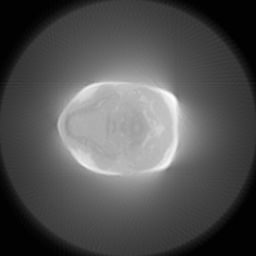
\includegraphics[width=0.3\textwidth]{Files/report_images/SUM_backprojections_k5.jpg}
            \caption{The filter used to weight the projections to remove the long tails that obscure the image.\label{fig:filtered_backprojection}}
        \end{figure}

        Because the filter is applied as a discrete kernel, the size must be chosen to compromise between speed and accuracy. This image in figure~\ref{fig:filtered_backprojection} shows a kernel size of $5\times 5$. The effect of increasing the kernel size can be seen below in figure~\ref{fig:kernel_sizes}.
        \begin{figure}[ht]
            \centering
            \begin{minipage}[c]{0.3\linewidth}
                \centering
                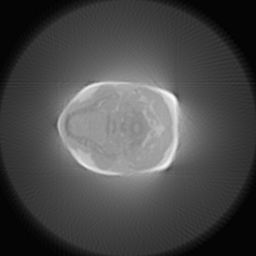
\includegraphics[width=\textwidth]{Files/report_images/SUM_backprojections_k7.jpg}
            \end{minipage}
            \begin{minipage}[c]{0.3\linewidth}
                \centering
                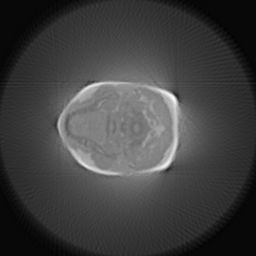
\includegraphics[width=\textwidth]{Files/report_images/SUM_backprojections_k9.jpg}
            \end{minipage}
            \begin{minipage}[c]{0.3\linewidth}
                \centering
                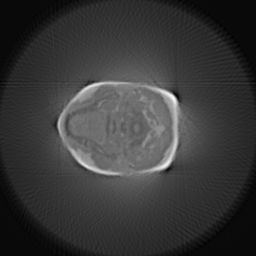
\includegraphics[width=\textwidth]{Files/report_images/SUM_backprojections_k11.jpg}
            \end{minipage}

            \begin{minipage}[c]{0.3\linewidth}
                \centering
                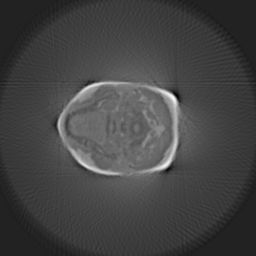
\includegraphics[width=\textwidth]{Files/report_images/SUM_backprojections_k13.jpg}
            \end{minipage}
            \begin{minipage}[c]{0.3\linewidth}
                \centering
                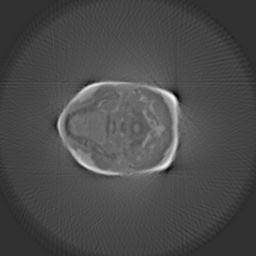
\includegraphics[width=\textwidth]{Files/report_images/SUM_backprojections_k15.jpg}
            \end{minipage}
            \caption{The images reconstructed using different sized kernels, from, top left to bottom right, $7\times 7$ to $15\times 15$.\label{fig:kernel_sizes}}
        \end{figure}

        As the kernel size increases, the change in image quality decreases as the tails of the Fourier Transform of the weighting function decrease away from the centre.
    % subsection applying_the_filter (end)

    \subsection{Tomographic Reconstruction} % (fold)
    \label{sub:tomographic_reconstruction}
        We have seen how a tomographic scan can be used to reconstruct a particular slice through an object using both simple back projection, and by employing the central slice theorem to allow the errors, in the form of long tails that obscure the image, to be reduced. The image that is arrived at is not as clear as the image that was aimed for, figure~\ref{fig:reference_slice}, as these tails cannot be removed completely due to the finite kernel used to reduce them.
    % subsection tomographic_reconstruction (end)


% section central_slice_theorem (end)

